% Este documento tem a ver com as partes do LIVRO. 

% Tamanhos
% \tiny
% \scriptsize
% \footnotesize
% \small 
% \normalsize
% \large 
% \Large 
% \LARGE 
% \huge
% \Huge

% Posicionamento
% \centering 
% \raggedright
% \raggedleft
% \vfill 
% \hfill 
% \vspace{Xcm}   % Colocar * caso esteja no começo de uma página. Ex: \vspace*{...}
% \hspace{Xcm}

% Estilo de página
% \thispagestyle{<<nosso>>}
% \thispagestyle{empty}
% \thispagestyle{plain}  (só número, sem cabeço)
% https://www.overleaf.com/learn/latex/Headers_and_footers

% Compilador que permite usar fonte de sistema: xelatex, lualatex
% Compilador que não permite usar fonte de sistema: latex, pdflatex

% Definindo fontes
% \setmainfont{Times New Roman}  % Todo o texto
% \newfontfamily\avenir{Avenir}  % Contexto

\begingroup\thispagestyle{empty}

\begin{textblock*}{2.625in}(0pt,0pt)%
\vspace*{-3.5cm}
%\hspace*{-4cm}
\includegraphics[scale=1]{../watermarks/front5ano.pdf}
\end{textblock*}
                
              \vspace*{\fill}
              \begin{center}
              {\HUGE\textbf{Revisa SAEB}}\bigskip

              {\LARGE\textbf{2º ano: Matemática}}

              \bigskip
              \bigskip
              \bigskip

              {\Large
                            AUTORIA

                            }
              \end{center}
              \vspace*{\fill}

\endgroup
\pagebreak       % [Frontistício]
%\newcommand{\linhalayout}[2]{{\tiny\textbf{#1}\quad#2\par}}
\newcommand{\linha}[2]{\ifdef{#2}{\linhalayout{#1}{#2}}{}}

\begingroup\tiny
\parindent=0cm
\thispagestyle{empty}

\textbf{Gerência editorial}\quad			 {Ana Mortara}\\
\textbf{Assistência editorial}\quad			 {Paula Dias}\\
\textbf{Assistência administrativa editorial}\quad {Gisele Cerchiaro}\\

\hspace{-5pt}\begin{tabular}{ll}
\textbf{Elaboração de conteúdo} & Abraão Augusto (Língua Portuguesa),	\\
								& Alessandra Domingues Juliano (Língua Portuguesa),	\\
								& Ana Paula Souza Rios (Língua Portuguesa),	\\
								& André Sanchez Astorino (Língua Portuguesa e Língua Inglesa),	\\
								& Clarissa Ayres Mendes (Língua Portuguesa),	\\
								& Eduardo Toniolo Campos (Matemática),	\\
								& Fernanda Dobashi (Língua Portuguesa),	\\
								& Guilherme Salles (Ciências Humanas),	\\
								& Letícia Leme (Ciências Humanas),	\\
								& Lucas Della Santina (Educação Física),	\\
								& Pilar Espí (Arte),	\\
								& Renata Cândido Carvalho (Ciências da Natureza),	\\
								& Thiago Figueiredo (Matemática),	\\
								& Victor Marques (Ciências da Natureza)	\\
\end{tabular}


\textbf{Edição}\quad	 {Carlos Rogério Duarte Barreiros, Fábia Alvim, Felipe Augusto Neves Silva}\\
\textbf{Preparação e revisão}\quad			 {Saíra Editorial}\\
\textbf{Coordenação de arte}\quad			 {Jorge Sallum}\\
\textbf{Editoração eletrônica}\quad			 {Paulo Henrique Pompermaier}\\
\textbf{Pesquisa iconográfica}\quad			 {Margarita Veloso}\\
\textbf{Projeto gráfico e capa}\quad		 {Luísa Marcelino}\\
\textbf{Código}\quad {\ifdef{\RevisionInfo{}}{\RevisionInfo{} (\today, \currenttime)}{001}\medskip}

\noindent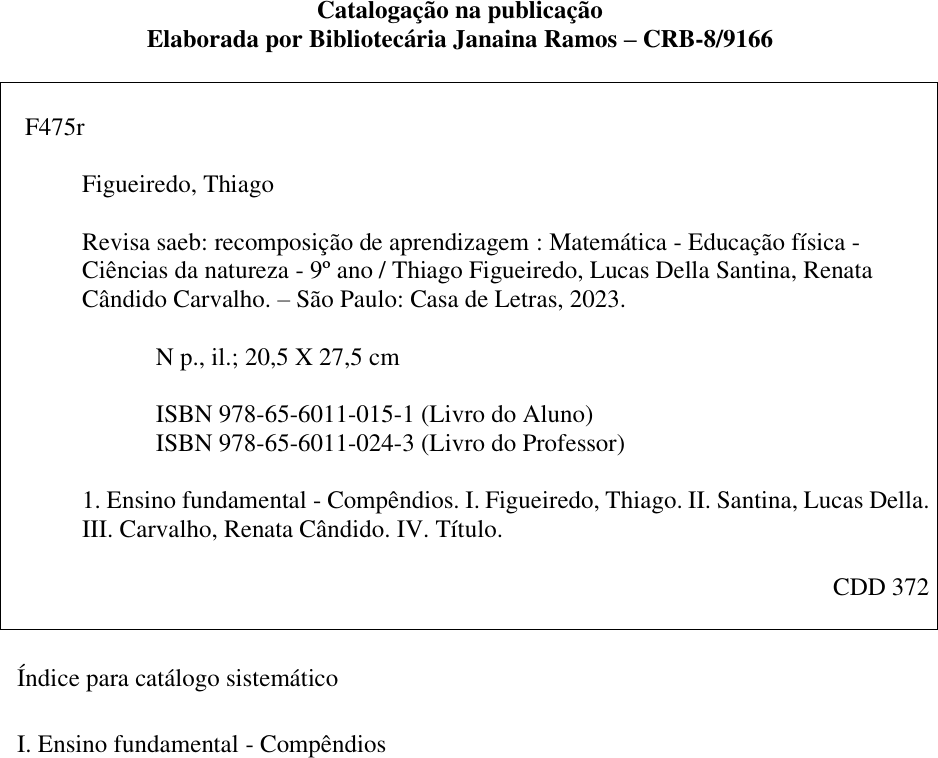
\includegraphics[width=.5\textwidth]{../fichas/9MAT.png}

\vfill

\textsc{casa de letras e gráfica ltda.}\\
Rua Fradique Coutinho, 1139, andar 2, sala 2\\
CEP 05416--011 -- São Paulo/\textsc{sp}, Brasil\\
Telefone: (11) 3914--7790\\\smallskip
www.casadeletras.com.br\\

\endgroup
\pagebreak
     % [Créditos]
% nothing			is level -3
% \book				is level -2
% \part				is level -1
% \chapter 			is level 0
% \section 			is level 1
% \subsection 		is level 2
% \subsubsection 	is level 3
% \paragraph 		is level 4
% \subparagraph 	is level 5
\setcounter{secnumdepth}{2}
\setcounter{tocdepth}{0}
 
% \renewcommand{\contentsname}{Índex} 	% Trocar nome do sumário para 'Índex'
%\ifodd\thepage\relax\else\blankpage\fi 	% Verifica se página é par e coloca página branca
%\tableofcontents*

\pagebreak
{\begingroup\mbox{}\pagestyle{empty}
\pagestyle{empty} 
% \renewcommand{\contentsname}{Índex} 	% Trocar nome do sumário para 'Índex'
%\ifodd\thepage\relax\else\blankpage\fi 	% Verifica se página é par e coloca página branca
\addtocontents{toc}{\protect\thispagestyle{empty}}
\addtocontents{toc}{\vspace*{-1cm}}
\tableofcontents*\clearpage\endgroup}

%\newwatermark[pagex={4}]{\vspace{2.5cm}\hspace*{7.8cm}
\includegraphics[scale=1]{../watermarks/intro5ano.pdf}}

\newwatermark[pagex={6,142,166}]{\vspace{2.5cm}\hspace*{7.8cm}
\includegraphics[scale=1]{../watermarks/1modulo5ano.pdf}}
\newwatermark[pagex={16,148}]{\vspace{2.5cm}\hspace*{7.8cm}
\includegraphics[scale=1]{../watermarks/2modulo5ano.pdf}}
\newwatermark[pagex={175}]{\vspace{2.5cm}\hspace*{7.8cm}
\includegraphics[scale=1]{../watermarks/2modulo5ano_impar.pdf}}
\newwatermark[pagex={24}]{\vspace{2.5cm}\hspace*{7.8cm}
\includegraphics[scale=1]{../watermarks/3modulo5ano.pdf}}
\newwatermark[pagex={155,185}]{\vspace{2.5cm}\hspace*{7.8cm}
\includegraphics[scale=1]{../watermarks/3modulo5ano_impar.pdf}}
\newwatermark[pagex={32}]{\vspace{2.5cm}\hspace*{7.8cm}
\includegraphics[scale=1]{../watermarks/4modulo5ano.pdf}}
\newwatermark[pagex={39}]{\vspace{2.5cm}\hspace*{7.8cm}
\includegraphics[scale=1]{../watermarks/5modulo5ano_impar.pdf}}
\newwatermark[pagex={50}]{\vspace{2.5cm}\hspace*{7.8cm}
\includegraphics[scale=1]{../watermarks/6modulo5ano.pdf}}
\newwatermark[pagex={59}]{\vspace{2.5cm}\hspace*{7.8cm}
\includegraphics[scale=1]{../watermarks/7modulo5ano_impar.pdf}}
\newwatermark[pagex={65}]{\vspace{2.5cm}\hspace*{7.8cm}
\includegraphics[scale=1]{../watermarks/8modulo5ano_impar.pdf}}
\newwatermark[pagex={78}]{\vspace{2.5cm}\hspace*{7.8cm}
\includegraphics[scale=1]{../watermarks/9modulo5ano.pdf}}
\newwatermark[pagex={88}]{\vspace{2.5cm}\hspace*{7.8cm}
\includegraphics[scale=1]{../watermarks/10modulo5ano.pdf}}
\newwatermark[pagex={95}]{\vspace{2.5cm}\hspace*{7.8cm}
\includegraphics[scale=1]{../watermarks/11modulo5ano_impar.pdf}}
\newwatermark[pagex={102}]{\vspace{2.5cm}\hspace*{7.8cm}
\includegraphics[scale=1]{../watermarks/12modulo5ano.pdf}}
\newwatermark[pagex={111}]{\vspace{2.5cm}\hspace*{7.8cm}
\includegraphics[scale=1]{../watermarks/13modulo5ano_impar.pdf}}
\newwatermark[pagex={119}]{\vspace{2.5cm}\hspace*{7.8cm}
\includegraphics[scale=1]{../watermarks/14modulo5ano_impar.pdf}}
\newwatermark[pagex={127}]{\vspace{2.5cm}\hspace*{7.8cm}
\includegraphics[scale=1]{../watermarks/15modulo5ano_impar.pdf}}

\newwatermark[pagex={5,7,9,11,13,15,17,19,21,23,25,27,29,31,33,35,37,39,41,43,45,47,49,51,53,55,57,59,61,63,65,67,69,71,73,75,77,79,81,83,85,87,89,91,93,95,97,99,101,103,105,107,109,111,113,115,117,119,121,123,125,127,129,131,133,135,137,139,143,145,147,149,151,153,155,157,159,161,167,169,171,173,175,177,179,181,183,185,187,189,191}]{\vspace{2.5cm}\hspace*{8cm}
\includegraphics[scale=1]{../watermarks/bg5anoimpar.pdf}}

\newwatermark[pagex={8,10,12,14,16,18,20,22,26,28,30,32,34,36,38,40,42,44,46,48,50,52,54,56,58,60,62,64,66,68,70,72,74,76,78,80,82,84,86,88,90,92,94,96,98,100,102,104,106,108,110,112,114,116,118,120,122,124,126,128,130,132,134,136,138,144,146,148,150,152,154,156,158,160,162,168,170,172,174,176,178,180,182,184,186,188,190,192}]{\vspace{2.5cm}\hspace*{7.8cm}
\includegraphics[scale=1]{../watermarks/bg5anopar.pdf}}

\newwatermark[pagex={195,197,199,201,203,207,209,211,213,215,219,221,223,225,227,231,233,235,237,239,241,243}]{\vspace{2.5cm}\hspace*{8cm}
\includegraphics[scale=1]{../watermarks/bgsim5anoimpar.pdf}}

\newwatermark[pagex={194,196,198,200,202,204,206,208,210,212,214,218,220,222,224,226,228,230,232,234,236,238,240,242,244}]{\vspace{2.5cm}\hspace*{7.8cm}
\includegraphics[scale=1]{../watermarks/bgsim5anopar.pdf}}
%!TEX root=./LIVRO.tex
\chapter{APRESENTAÇÃO}

O \textbf{SISTEMA DE AVALIAÇÃO DA EDUCAÇÃO BÁSICA (SAEB)} É UM CONJUNTO
DE AVALIAÇÕES EXTERNAS EM LARGA ESCALA QUE PERMITE AO INSTITUTO NACIONAL
DE ESTUDOS E PESQUISAS EDUCACIONAIS ANÍSIO TEIXEIRA (INEP) REALIZAR UM
DIAGNÓSTICO DA EDUCAÇÃO BÁSICA BRASILEIRA E DE FATORES QUE PODEM
INTERFERIR NO DESEMPENHO DOS ESTUDANTES.

POR MEIO DE TESTES E QUESTIONÁRIOS, APLICADOS A CADA DOIS ANOS NA REDE
PÚBLICA E EM UMA AMOSTRA DA REDE PRIVADA, O SAEB REFLETE OS NÍVEIS DE
APRENDIZAGEM DEMONSTRADOS PELOS ESTUDANTES AVALIADOS, EXPLICANDO ESSES
RESULTADOS A PARTIR DE UMA SÉRIE DE INFORMAÇÕES CONTEXTUAIS.

O SAEB PERMITE QUE AS ESCOLAS E AS REDES MUNICIPAIS E ESTADUAIS DE
ENSINO AVALIEM A QUALIDADE DA EDUCAÇÃO OFERECIDA AOS ESTUDANTES. O
RESULTADO DA AVALIAÇÃO É UM INDICATIVO DA QUALIDADE DO ENSINO BRASILEIRO
E OFERECE SUBSÍDIOS PARA ELABORAÇÃO, MONITORAMENTO E APRIMORAMENTO DE
POLÍTICAS EDUCACIONAIS, SEMPRE COM BASE EM EVIDÊNCIAS.

AS MÉDIAS DE DESEMPENHO DOS ESTUDANTES, APURADAS NO SAEB, JUNTAMENTE COM
AS TAXAS DE APROVAÇÃO, REPROVAÇÃO E ABANDONO, APURADAS NO CENSO ESCOLAR,
COMPÕEM O ÍNDICE DE DESENVOLVIMENTO DA EDUCAÇÃO BÁSICA (IDEB).

REALIZADO DESDE 1990, O SAEB PASSOU POR UMA SÉRIE DE APRIMORAMENTOS
TEÓRICO-METODOLÓGICOS AO LONGO DAS EDIÇÕES. A EDIÇÃO DE 2019 MARCA O
INÍCIO DE UM PERÍODO DE TRANSIÇÃO ENTRE AS MATRIZES DE REFERÊNCIA
UTILIZADAS DESDE 2001 E AS NOVAS MATRIZES ELABORADAS EM CONFORMIDADE COM
A BASE NACIONAL COMUM CURRICULAR (BNCC).

\section*{REVISA SAEB: REFORÇO ESCOLAR}

COMO O PRÓPRIO NOME DIZ, A EDUCAÇÃO BÁSICA É AQUELA EM QUE SE PROMOVE A
FORMAÇÃO MAIS ESSENCIAL DOS ALUNOS. O SISTEMA DE AVALIAÇÃO DA EDUCAÇÃO
BÁSICA (SAEB) AJUDA NA DETECÇÃO DOS PONTOS FORTES E FRACOS NA FORMAÇÃO
DOS ALUNOS EM ESTADOS, EM MUNICÍPIOS, EM ESCOLAS, FUNCIONANDO COMO UM
PARÂMETRO PARA QUE PROBLEMAS SEJAM SOLUCIONADOS E PARA QUE, ANO APÓS
ANO, ESSA FORMAÇÃO EVOLUA E AJUDE NO CRESCIMENTO DESSAS ESCOLAS, DESSES
MUNICÍPIOS E DESSES ESTADOS.

A PREPARAÇÃO ADEQUADA PARA AVALIAÇÕES EM LARGA ESCALA, COMO A DO SAEB, É
IMPORTANTE PARA QUE, NO MOMENTO DA PROVA, OS ALUNOS POSSAM ESTAR ATENTOS
E TRANQUILOS PARA DAREM O MELHOR POSSÍVEL DE SEU POTENCIAL. ASSIM, UM
MATERIAL DIDÁTICO DE APOIO QUE, DE FATO, PROMOVA ESSA PREPARAÇÃO É O
MAIOR DOS ALIADOS PARA PROFESSORES E GESTORES. ESTE MATERIAL TEM
EXATAMENTE ESTA INTENÇÃO: GARANTIR UM MELHOR APROVEITAMENTO DE CADA
ESTUDANTE NA RESOLUÇÃO DE ATIVIDADES, PARA QUE CONSIGAM RESULTADOS
EXCELENTES NESSA TRAJETÓRIA DE AVALIAÇÃO.

O \textbf{REVISA SAEB} ESTÁ DIVIDIDO EM 18 VOLUMES, DISTRIBUÍDOS, AO
LONGO DO ENSINO FUNDAMENTAL, DA SEGUINTE MANEIRA:

\begin{itemize}
\item
  NOS ANOS INICIAIS, PARA O \textbf{PRIMEIRO}, O \textbf{SEGUNDO}, O
  \textbf{TERCEIRO} E O \textbf{QUARTO ANO}, E NOS ANOS FINAIS, PARA O
  \textbf{SEXTO}, O \textbf{SÉTIMO} E O \textbf{OITAVO ANO}, EXISTE UM
  VOLUME POR ANO DE LÍNGUA PORTUGUESA E EXISTE UM VOLUME POR ANO DE
  MATEMÁTICA.
\item
  O \textbf{QUINTO ANO} APRESENTA UMA ESTRUTURA ESPECIAL. EM UM VOLUME,
  APARECEM ESTES COMPONENTES: LÍNGUA PORTUGUESA, ARTE E CIÊNCIAS
  HUMANAS. EM OUTRO VOLUME, APARECEM ESTES COMPONENTES: MATEMÁTICA,
  EDUCAÇÃO FÍSICA E CIÊNCIAS DA NATUREZA.
\item
  O \textbf{NONO ANO} TAMBÉM APRESENTA UMA ESTRUTURA ESPECIAL. SÃO DOIS
  VOLUMES: UM CONTÉM LÍNGUA PORTUGUESA, ARTE, LÍNGUA INGLESA E CIÊNCIAS
  HUMANAS; O OUTRO CONTÉM MATEMÁTICA, EDUCAÇÃO FÍSICA E CIÊNCIAS DA
  NATUREZA.
\end{itemize}

CADA VOLUME, EM CADA COMPONENTE, ESTÁ DIVIDIDO EM MÓDULOS TEMÁTICOS (DE
UMA OU DUAS AULAS), E CADA MÓDULO CONTA COM A ESTRUTURA DESCRITA A
SEGUIR.

\begin{itemize}
\item
  A \textbf{ABERTURA DO MÓDULO} APRESENTA UM RESUMO TEÓRICO DE
  CONTEXTUALIZAÇÃO, VINCULADO, PRINCIPALMENTE, A HABILIDADES DAS
  MATRIZES DO SAEB, MAS TAMBÉM A ALGUMAS HABILIDADES DA BNCC QUE TÊM
  RELAÇÃO COM ESSAS PRIMEIRAS HABILIDADES.
\item
  NA SEQUÊNCIA, ABRE-SE UMA SEÇÃO DE \textbf{ATIVIDADES}, QUE CONTÉM
  EXERCÍCIOS DE MODELOS VARIADOS PARA RETOMADA E FIXAÇÃO
  DO CONTEÚDO TRAZIDO PELO MÓDULO.
\item
  NO FECHAMENTO DE CADA MÓDULO, SURGE UMA SEÇÃO CHAMADA \textbf{TREINO},
  QUE CONTÉM TRÊS ITENS (QUESTÕES NO MODELO DO INEP, QUE É O MESMO
  UTILIZADO NOS TESTES COGNITIVOS DO SAEB). CADA ITEM CHECA O
  DESENVOLVIMENTO DE UMA HABILIDADE DAS MATRIZES DO SAEB E, SEMPRE QUE
  HÁ CONEXÃO, ESTÁ VINCULADO A UMA HABILIDADE DA BNCC DO ANO
  CORRESPONDENTE.
\item
  OS VOLUMES SE ENCERRAM COM QUATRO \textbf{SIMULADOS}, PARA SEREM
  APLICADOS BIMESTRALMENTE. AO LONGO DOS QUATROS SIMULADOS, TODAS AS
  HABILIDADES DAS MATRIZES DO SAEB, EM CADA ANO, SÃO TRABALHADAS, DESDE
  QUE VINCULADAS A CONTEÚDOS PREVISTOS PELA BNCC PARA O ANO EM
  ESPECÍFICO. IGUALMENTE COMPOSTOS DE ITENS, EM NÚMEROS VARIADOS, OS
  SIMULADOS TAMBÉM APRESENTAM, SEMPRE QUE HÁ CONEXÃO, HABILIDADES DA
  BNCC.
\end{itemize}

\addcontentsline{toc}{chapter}{PORTUGUÊS}
\pagestyle{por}
\chapter[O alfabeto, as vogais e as consoantes]{\Large O alfabeto, as vogais e as consoantes}
\markboth{Módulo 1}{}

\colorsec{Habilidade do SAEB}

\begin{itemize}
\item Relacionar elementos sonoros das palavras com sua representação escrita.
\end{itemize}

\colorsec{Habilidade da BNCC}

\begin{itemize}
\item EF02LP03.
\end{itemize}

\conteudo{Para escrever as palavras, usamos as \textbf{letras}. 
Juntas, elas compõem o \textbf{alfabeto}, que é formado por 26 letras. 

As \textbf{vogais} são \textit{a, e, i, o, u}, e as outras letras são
chamadas de \textbf{consoantes}. Veja:

\begin{myquote}
b c d f g h j k l m n p q r s t v w x y z
\end{myquote}

Cada letra possui um nome e um som, que, quando estão juntos, podem
formar muitas palavras.

\begin{longtable}[]{@{}llllll@{}}
\toprule
\textbf{PATO} & \textbf{VACA} & \textbf{BOLA} & \textbf{TATU} &
\textbf{FADA} & \textbf{DOCE}\tabularnewline
\bottomrule
\end{longtable}

A letra C pode apresentar dois sons diferentes de acordo com a vogal que
acompanha. Por exemplo: junto com as vogais A, O e U, apresenta o som de 
/k/; junto com E e I apresenta o som de /s/.
}
 
%Felipe: precisamos padronizar como vamos grafar as letras e os fonemas, como ocorreu na frase acima. (Rogério, 13/3/23, 14h31)

\conteudo{
Algumas palavras com o som de /k/ também podem ser escritas com Q,
mas vale lembrar que o Q vem sempre acompanhado de U e de mais uma
vogal, e é esta última vogal que vai marcar o som da sílaba. Observe:

\begin{center}
\begin{tabular}{l}
\hline
\textbf{PALAVRAS C COM SOM DE /K/} \\ \hline
\textbf{CUCA} \\
\textbf{CASA} \\
\textbf{COCO} \\ \hline
\textbf{PALAVRAS C COM SOM DE /S/} \\ \hline
\textbf{CEBOLA} \\
\textbf{CINCO} \\
\textbf{CISNE} \\ \hline
\textbf{PALAVRAS COM QU} \\ \hline
\textbf{QUEIJO} \\
\textbf{QUILO} \\
\textbf{QUERO} \\
\textbf{QUIBE}
\end{tabular}
\end{center}

Veja a grafia dessas palavras.

\begin{myquote}
TATU \hspace{2cm}  GALO 
\end{myquote}

Na grafia das palavras com as vogais O e U, o O no final de palavras é
fraco, e o U é sempre forte.

\begin{quote}
A letra /k/ é usada apenas em situações como nomes de
pessoas, como Kátia, e palavras estrangeiras como
\textit{ketchup, kit, kibon} e \textit{kaiser}.
\end{quote}
}

\pagebreak
\colorsec{Atividades}

\num{1} Complete os nomes das figuras com as letras que estão faltando.

\begin{figure}[htpb!]

\includegraphics[width=.5\textwidth]{media/image1.jpeg}
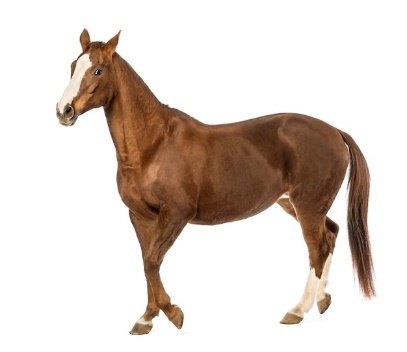
\includegraphics[width=.5\textwidth]{media/image2.jpeg}
\end{figure}

T \reduline{A} P \reduline{E} T \reduline{E}\hspace{6cm} C \reduline{A} V \reduline{A} L \reduline{O}


\begin{figure}[htpb!]

\includegraphics[width=.5\textwidth]{media/image3.jpeg}

\includegraphics[width=.5\textwidth]{media/image4.jpeg}
\end{figure}

\reduline{E} STR \reduline{E} L \reduline{A} \hspace{6cm} P \reduline{O} RT \reduline{A}

\pagebreak
Você completou as palavras com

\begin{boxlist}
\boxitem{\white{X}} Vogais 

\boxitem{\white{X}} Consoantes
\end{boxlist}

%\coment{Apresente as vogais em cartaz. Pergunte o nome dos objetos representados nas imagens e, em seguida, convide as crianças para montar as palavras no alfabeto móvel para identificar as letras faltantes.}

\num{2} Complete o alfabeto com as letras que estão faltado.

\begin{center}
\Large
\begin{tabular}{|l|l|llllll}
\hline
\textbf{A} & \rosa{B} & \multicolumn{1}{l|}{\rosa{C}} & \multicolumn{1}{l|}{\rosa{D}} & \multicolumn{1}{l|}{\textbf{E}} & \multicolumn{1}{l|}{\rosa{F}} & \multicolumn{1}{l|}{\rosa{G}} & \multicolumn{1}{l|}{\rosa{H}} \\ \hline
\textbf{I} & \rosa{J} & \multicolumn{1}{l|}{\rosa{K}} & \multicolumn{1}{l|}{\rosa{L}} & \multicolumn{1}{l|}{\rosa{M}} & \multicolumn{1}{l|}{\rosa{N}} & \multicolumn{1}{l|}{\textbf{O}} & \multicolumn{1}{l|}{\rosa{P}} \\ \hline
\rosa{Q} & \rosa{R} & \multicolumn{1}{l|}{\rosa{S}} & \multicolumn{1}{l|}{\rosa{T}} & \multicolumn{1}{l|}{\textbf{U}} & \multicolumn{1}{l|}{\rosa{V}} & \multicolumn{1}{l|}{\rosa{W}} & \multicolumn{1}{l|}{\rosa{X}} \\ \hline
\rosa{Y} & \rosa{Z} & \textbf{} & \textbf{} & \textbf{} & \textbf{} & \textbf{} & \textbf{} \\ \cline{1-2}
\end{tabular}
\end{center}

Você completou as palavras com:

\begin{boxlist}
\boxitem{\white{X}} Vogais 

\boxitem{\white{X}} Consoantes
\end{boxlist}

%\coment{Leve o alfabeto móvel para sala e convide os alunos para organizar as letras na ordem certa. Em seguida, oriente-os a preencher o quadro; depois ajude a separar vogais e consoantes.}

\num{3} Leia o poema.

\textbf{A vaca Filomena e a formiga Violeta}


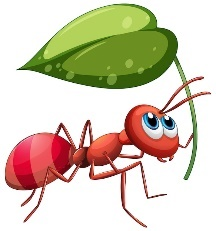
\includegraphics[width=.2\textwidth]{media/image5.jpeg}

\includegraphics[width=.3\textwidth]{media/image6.jpeg}

\begin{verse}
A vaca Filomena\\
mora na vila formosa.\\
A formiga Violeta\\
mora na cerca cor de rosa.

\pagebreak
A vaca Filomena\\
come as uvas da parreira.\\
A formiga Violeta\\
acha isto uma besteira.
\end{verse}

\fonte{Isabel Cristina Silveira Soares. https://seceducacao.padua.rj.gov.br/wp-content/uploads/2021/05/3o-ano-Ling.-Portuguesa-ATIV.17.pdf.
Acesso 28 de Fev 2023.}

Encontre e pinte no texto todas as palavras iniciadas com F e V. 
Depois escreva abaixo as palavras que encontrou.

\reduline{As palavras encontradas são as seguintes: vaca, Filomena, vila,
formosa, formiga, violeta.
Leve as palavras \textit{vaca} e \textit{formiga} em uma caixinha e
apresente-as para as crianças. Faça a leitura das palavras e estimule 
questionamentos sobre esses animais: os alunos sabem como eles são?
Onde esses animais vivem? Que sons eles emitem? Faça com os
alunos a leitura do poema e oriente a localização das palavras iniciadas
com as consoantes V e F.\hfill}

\num{4} Complete os espaços a seguir com as letras iniciais das palavras
\textit{violeta} e \textit{filomena}.

%\coment{Leve as palavras Violeta e Filomena em um cartaz. Explore a letra inicial e o som da letra nas palavras.}

\begin{figure}[htpb!]

\includegraphics[width=.3\textwidth]{media/image7.jpeg}

\includegraphics[width=.3\textwidth]{media/image8.jpeg}

\includegraphics[width=.3\textwidth]{media/image9.jpeg}
\end{figure}

\reduline{F} ACA \hspace{4cm} \reduline{F} ADA \hspace{3cm} \reduline{V} ELA

\pagebreak
\begin{figure}[htpb!]
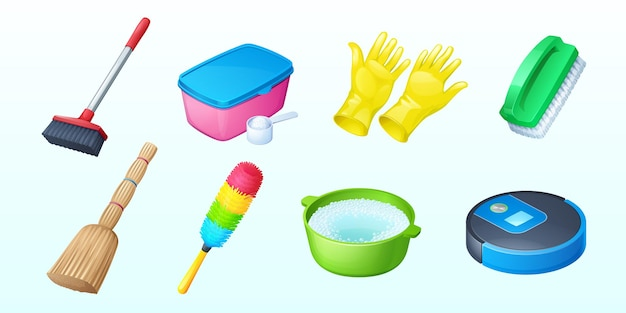
\includegraphics[width=.3\textwidth]{media/image10.jpeg}

\includegraphics[width=.3\textwidth]{media/image11.jpeg}

\includegraphics[width=.3\textwidth]{media/image12.jpeg}
\end{figure}

 \reduline{V} ASSOURA \hspace{4cm} \reduline{F} OGO \hspace{3cm} \reduline{F} IVELA

\begin{figure}[htpb!]
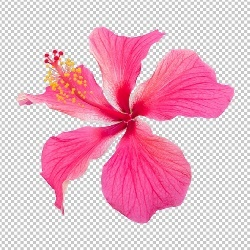
\includegraphics[width=.3\textwidth]{media/image13.jpeg}

\includegraphics[width=.3\textwidth]{media/image14.jpeg}

\includegraphics[width=.3\textwidth]{media/image15.jpeg}
\end{figure}

\reduline{F} LOR \hspace{4cm} \reduline{F} OGUETE \hspace{3cm} SOR \reduline{V} ETE


\num{5} Pinte as iniciais de cada palavra.

%\coment{Leve para sala palavras iniciadas pelas letras T, D, F, V, B, P. Convide as crianças para fazer a leitura, identificado o som das letras iniciais e finais, e quantidade de sílabas. Também é possível trabalhar a função social da escrita das palavras}.

\begin{center}
\begin{tabular}{|c|c|c|c|c|}
\hline
\textbf{VACINA} & F & T & D & \rosa{V} \\ \hline
\textbf{TESOURA} & P & D & \rosa{T} & F \\ \hline
\textbf{VASSOURA} & B & T & \rosa{V} & F \\ \hline
\textbf{FACA} & V & \rosa{F} & D & T \\ \hline
\textbf{DEDO} & T & V & F & \rosa{D} \\ \hline
\textbf{PANELA} & V & T & \rosa{P} & B \\ \hline
\textbf{DOMINÓ} & B & \rosa{D} & T & P \\ \hline
\textbf{BONECA} & F & P & \rosa{B} & D \\ \hline
\end{tabular}
\end{center}

\pagebreak
\num{6} Numere os desenhos conforme os números das palavras.

%\coment{Faça leitura das palavras com as crianças, de modo que elas identifiquem a numeração e façam a associação correta.}

\begin{multicols}{3}
\begin{enumerate}
\item BOLA

\item FOCA

\item TATU

\item PANELA

\item TAPETE

\item FORMIGA

\item DADO

\item VACA

\item PATO

\item BONECA
\end{enumerate}
\end{multicols}

\begin{longtable}[]{@{}llll@{}}
\reduline{\_\_10\_\_} &

\includegraphics[width=1.16667in,height=0.96319in]{media/image16.jpeg} &
\reduline{\_\_8\_\_} &

\includegraphics[width=1.16127in,height=0.95833in]{media/image17.jpeg}\tabularnewline
\reduline{\_\_2\_\_} &

\includegraphics[width=1.09375in,height=1.09375in]{media/image18.jpeg} &
\reduline{\_\_4\_\_} &
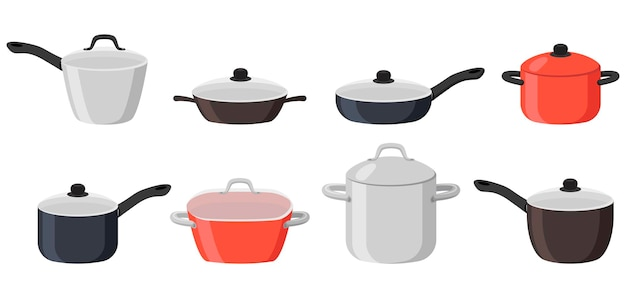
\includegraphics[width=1.27986in,height=0.98958in]{media/image19.jpeg}\tabularnewline
\reduline{\_\_3\_\_} &
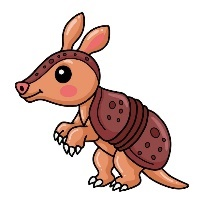
\includegraphics[width=0.92708in,height=0.92708in]{media/image20.jpeg} &
\reduline{\_\_6\_\_} &
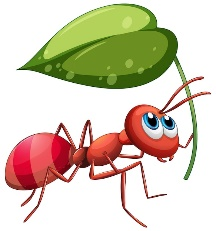
\includegraphics[width=0.97986in,height=1.05208in]{media/image21.jpeg}\tabularnewline
\reduline{\_\_1\_\_} &

\includegraphics[width=1.13542in,height=1.13542in]{media/image22.jpeg} &
\reduline{\_\_7\_\_} &

\includegraphics[width=1.23958in,height=1.15833in]{media/image23.jpeg}\tabularnewline
\reduline{\_\_9\_\_} &
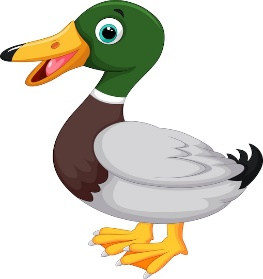
\includegraphics[width=1.19722in,height=1.27083in]{media/image24.jpeg} &
\reduline{\_\_5\_\_} &

\includegraphics[width=2.21875in,height=1.11458in]{media/image25.jpeg}\tabularnewline
\end{longtable}

\pagebreak
\num{7} Complete as palvaras com \textbf{-ca -co -cu} ou \textbf{-qua -que -qui}.

%\coment{Convide as crianças a falar o nome das imagens para identificar a grafia da palavra.}

\begin{figure}[htpb!]

\includegraphics[width=.24\textwidth]{media/image26.jpeg}
\includegraphics[width=.24\textwidth]{media/image27.jpeg}
\includegraphics[width=.24\textwidth]{media/image28.jpeg}
\includegraphics[width=.24\textwidth]{media/image29.jpeg}
\end{figure}

\reduline{CU} TIA \hspace{2cm} \reduline{CA} SA \hspace{2cm} \reduline{CU} SCUZ \hspace{2cm} \reduline{QUE} IJO

\begin{figure}[htpb!]
\includegraphics[width=.24\textwidth]{media/image30.jpeg}
\includegraphics[width=.24\textwidth]{media/image31.jpeg}
\includegraphics[width=.24\textwidth]{media/image32.jpeg}
\includegraphics[width=.24\textwidth]{media/image33.jpeg}
\end{figure}

A \reduline{QUÁ} RIO \hspace{1cm} \reduline{QUI} NZE \hspace{1cm} RA \reduline{QUE} TE \hspace{1cm} \reduline{CO} LA


\num{8} Encontre a sílaba mais forte e complete com O ou U.

%\coment{Leve para a classe uma caixinha enfeitada com palavras terminadas com O e U. Passe a caixinha para os alunos em círculo, ao som de uma música. Quando a música parar, o aluno que estiver com a caixinha na mão deve ler a palavra observando a letra  final. Em seguida, convide toda a turma a pronunciar a palavra e, então, descobrir a sílaba forte. Explique como descobrir quando a sílaba é forte e fraca, ensinando que, quando o U está no final, ele é sempre forte, e que o O é sempre fraco no final das palavras.}

\begin{figure}[htpb!]
\includegraphics[width=.3\textwidth]{media/image34.jpeg}
\includegraphics[width=.3\textwidth]{media/image35.jpeg}
\includegraphics[width=.2\textwidth]{media/image36.jpeg}
\end{figure}

SAPAT \reduline{O} \hspace{3cm} VAS \reduline{O} \hspace{2cm} TAT \reduline{U}

\begin{figure}[htpb!]
\includegraphics[width=.2\textwidth]{media/image37.jpeg}
\includegraphics[width=.3\textwidth]{media/image38.jpeg}
\includegraphics[width=.2\textwidth]{media/image39.jpeg}
\end{figure}

ESPELH \reduline{O} \hspace{1cm} CAJ \reduline{U} \hspace{2cm} CABEL \reduline{O}


\num{9} Pinte as palvras escritas com C que tem o som de S.
%Felipe: aqui precisamos padronizar, como comentei anteriormente. 

%\coment{Leve para sala palavras escritas com C. Organize uma roda de conversa na qual você orientará os alunos a organizar as palavras de acordo com a vogal que acompanha a letra C. Em seguida, explique a regra para descobrir se o C tem som de K ou S.}

\begin{longtable}[]{@{}lllll@{}}
\toprule
\textbf{CINEMA} & \textbf{CASA} & \textbf{CISNE} & \textbf{CEGO} &
\textbf{COCADA}\tabularnewline
\midrule
\endhead
\textbf{CADEIRA} & \textbf{CARRO} & \textbf{CINTO } & \textbf{COCO} &
\textbf{CAMA}\tabularnewline
\bottomrule
\end{longtable}

\num{10} Troque as letras e forme outras palavras.

%\coment{Utilize o alfabeto móvel com as palavras solicitadas no exercício e outras. Também é possível fazer a brincadeira da forca.}

\begin{longtable}[]{@{}lll@{}}
\toprule
\textbf{V POR F} & \textbf{D POR T} & \textbf{B POR P}\tabularnewline
\midrule
\endhead
\textbf{VACA} & \textbf{DADO} & \textbf{BODE}\tabularnewline
\textbf{\reduline{F}ACA} & \textbf{\reduline{T}ATO} & \textbf{\reduline{P}ODE}\tabularnewline
\textbf{VILA} & \textbf{DIA} & \textbf{BOTE}\tabularnewline
\textbf{\reduline{F}I LA} & \textbf{\reduline{T}IA} & \textbf{\reduline{P}OTE}\tabularnewline
\bottomrule
\end{longtable}

\pagebreak
\num{11} Complete a cruzadinha com o nome das figuras.

%\coment{Explore as frutas e legumes da atividade, fazendo questionamentos. Monte as palavras no alfabeto móvel com as crianças. Em seguida, oriente a escrita na cruzadinha.}

\begin{figure}[htpb!]
\includegraphics[width=\textwidth]{media/image40.png}
\end{figure}

\num{12} Encontre e pinte as palavras no diagrama.

%\coment{Depois da leitura das palavras, oriente os alunos a localizá-las no diagrama.}

\begin{longtable}[]{@{}llllllll@{}}
\toprule
	TATU -- CABELO -- BONECA -- PANELA -- CAJU\tabularnewline
FADA -- DADO -- VASO -- CAMA -- TAPETE\tabularnewline
\midrule
D & B & F & A & D & A & D & G\tabularnewline
A & C & A & B & E & L & O & U\tabularnewline
G & Y & B & O & C & A & M & A\tabularnewline
S & T & I & N & H & M & A & Q\tabularnewline
P & A & N & E & L & A & D & F\tabularnewline
H & T & O & C & A & J & U & L\tabularnewline
J & U & K & A & D & A & D & O\tabularnewline
T & A & P & E & T & E & Z & X\tabularnewline
K & V & A & S & O & B & G & J\tabularnewline
\end{longtable}

\pagebreak
\colorsec{Treino}

\num{1} Observe o animal que Júlia encontrou enquanto brincava na 
fazenda do Tio Belo.

\begin{figure}[htpb!]
\centering
\includegraphics[width=.9\textwidth]{media/image42.jpeg}
\end{figure}

A palavra que começa com a mesma letra do nome do animal que Júlia encontrou é

\begin{escolha}
\item vaso.

\item gato.

\item bola.

\item foca
\end{escolha}


\num{2} Observe a palavra que Tiago leu para sua professora.

\begin{myquote}
CAJU
\end{myquote}

O nome da figura que termina com a mesma letra da palavra que Tiago leu é

\begin{escolha}
\item\includegraphics[width=0.79792in,height=0.81667in]{media/image44.jpeg}

\item\includegraphics[width=1.02847in,height=0.72292in]{media/image45.jpeg}

\item\includegraphics[width=0.79792in,height=0.79931in]{media/image46.jpeg}

\item\includegraphics[width=1.08611in,height=0.97222in]{media/image47.jpeg}
\end{escolha}


\num{3} Observe o presente que Bruna ganhou.

\begin{figure}[htpb!]
\centering
\includegraphics[width=.3\textwidth]{media/image48.jpeg}
\end{figure}

A palavra que começa como o mesmo som da letra do nome do presente de Bruna é

\begin{multicols}{2}
\begin{escolha}
\item cama.

\item cubo.

\item cebola.

\item cocada.
\end{escolha}
\end{multicols}

\chapter{Lendo e escrevendo}
\markboth{Módulo 2}{}

\vspace*{-1.5cm}

\colorsec{Habilidades do SAEB}

\begin{itemize}
\item Ler palavras.
\item Escrever palavras.
\item Ler frases.
\end{itemize}

\colorsec{Habilidades da BNCC}

\begin{itemize}
\item EF02LP04, EF02LP05.
\end{itemize}

\conteudo{Para escrever uma palavra, você precisa usar as letras que
são chamadas de vogais e as consoantes.

As vogais são 

\begin{myquote}
\textbf{A -- E -- I -- O -- U} 
\end{myquote}

e as consoantes são

\begin{myquote}
\textbf{B -- C -- D -- F -- G -- H -- J -- K -- L -- M -- N -- P -- Q -- R -- S
-- T -- V -- W -- Y -- X -- Z.}
\end{myquote}

As palavras são lidas e escritas da esquerda para a direita.

\begin{myquote}
$\longrightarrow$

\textbf{GRAVIOLA LÂMPADA AVIÃO LARANJA }
\end{myquote}

Existem diferentes maneiras de compor a sílaba de uma palavra. 

\textbf{CONSOANTE + VOGAL}: é o que acontece nas três sílabas das 
palavras \textit{sapato} e \textit{telefone}: SA-PA-TO e TE-LE-FO-NE

\textbf{VOGAL}: é o que acontece na segunda sílaba das  
palavras \textit{saída} e \textit{saúde}: SA-Í-DA e SA-Ú-DE

\textbf{CONSOANTE + VOGAL + CONSOANTE}: é o que acontece na 
primera sílaba das palavras \textit{porta} e \textit{cortina}:
POR-TA e COR-TI-NA

\textbf{CONSOANTE + CONSOANTE + VOGAL}: é o que acontece na 
primera sílaba da palavra \textit{criança} e na última
sílaba da palavra \textit{livro}: CRI-AN-ÇA e LI-VRO 

Observe o quadro abaixo, com outros exemplos:\bigskip

\noindent{\tiny
\begin{tabular}{l|l|l|l|l|}
\cline{2-5}
 & \textbf{GRAVIOLA} & \textbf{LÂMPADA} & \textbf{AVIÃO} & \textbf{LARANJA} \\ \hline
\multicolumn{1}{|l|}{\textbf{FORMAÇÃO SILÁBICA CV}} & GRA - \textbf{VI} - O - \textbf{LA} & LÂM - \textbf{PA} - \textbf{DA} & A - \textbf{VI} -ÃO & \textbf{LA} - RAN - \textbf{JA} \\ \hline
\multicolumn{1}{|l|}{\textbf{FORMAÇÃO SILÁBICA V}} & GRA - VI - \textbf{O} - LA & \multicolumn{1}{c|}{*} & \textbf{A} - VI -ÃO & \multicolumn{1}{c|}{*} \\ \hline
\multicolumn{1}{|l|}{\textbf{FORMAÇÃO SILÁBICA CVC}} & \multicolumn{1}{c|}{*} & \textbf{LÂM} - PA - DA & \multicolumn{1}{c|}{*} & LA - \textbf{RAN} - JA \\ \hline
\multicolumn{1}{|l|}{\textbf{FORMAÇÃO SILÁBICA CCV}} & \textbf{GRA} - VI - O - LA & \multicolumn{1}{c|}{*} & \multicolumn{1}{c|}{*} & \multicolumn{1}{c|}{*} \\ \hline
\end{tabular}
}


Note que, em todas as formações das sílabas, aparecem vogais. Isso
acontece porque não existe sílaba sem vogal, isto é, uma  sílaba não
se forma só com consoantes.

Observe a frase a seguir:

\begin{myquote}
\textbf{O avião pousou cedo.}
\end{myquote}

Você conhece esse sinal em cima da letra A da palavra \textbf{avião}?

Esse sinal é o \textbf{til}, usado nas vogais A e O para marcar a
nasalidade presente na sílaba.

As marcas de nasalidade aparece também nas letras M e N, no final da
sílaba. É o que acontece, por exemplo, com as seguintes palavras:

\begin{myquote}
\textbf{LÂMPADA E LARANJA}
\end{myquote}

A letra \textbf{M} é utilizada antes das consoantes P e B.  
A letra \textbf{N} é usada antes das demais consoantes, nunca 
no final das palavras.
}

\colorsec{Atividades}

\num{1} Escreva os nomes das figuras.

%\coment{Leve o alfabeto móvel para a sala de aula. Convide as crianças para manusear as letras; em seguida, oriente-as a formar as palavras que nomeiam as figuras. Sugira a elas que, antes de escrever, elas devem pronunciar a palavra, escrevendo-a por sílabas ou pedacinhos.}


\begin{figure}[htpb!]
\includegraphics[width=1.46154in,height=0.93603in]{media/image49.jpeg}
\includegraphics[width=1.16587in,height=0.93269in]{media/image50.jpeg}
\includegraphics[width=1.42308in,height=1.21950in]{media/image51.jpeg}
\end{figure}

\reduline{Apito\hfill}

\reduline{Bicicleta\hfill}

\reduline{Árvore\hfill}

\begin{figure}[htpb!]
\includegraphics[width=1.10833in,height=1.00903in]{media/image52.jpeg}
\includegraphics[width=0.85556in,height=0.92222in]{media/image53.jpeg}
\includegraphics[width=0.79808in,height=0.79808in]{media/image54.jpeg}
\end{figure}

\reduline{Bola\hfill}

\reduline{Raposa\hfill}

\reduline{Gaiola\hfill}

\begin{figure}[htpb!]
\includegraphics[width=0.91319in,height=1.16319in]{media/image55.jpeg}
\includegraphics[width=1.62569in,height=1.25000in]{media/image56.jpeg}
\includegraphics[width=0.93990in,height=1.27885in]{media/image57.jpeg}
\end{figure}

\reduline{Pera\hfill}

\reduline{Pedra\hfill}

\reduline{Unha\hfill}

\pagebreak
\num{2} Separe as sílabas das palavras, depois circule as sílabas formadas por
consoante + consoante + vogal.

%\coment{Leia as palavras com os alunos, orientando-os a identificar vogais e consoantes. Também é possível montar algumas palavras com o alfabeto móvel. Em seguida, peça a eles que batam palmas cada vez que um pedacinho da palavra for pronunciado.}

\begin{longtable}[]{@{}ll@{}}
\toprule
\textbf{PRATO} & \rosa{Pra - to}\tabularnewline
\midrule
\textbf{FORMIGA} & \rosa{For- mi -ga}\tabularnewline
\midrule
\textbf{BRAÇO} & \rosa{Bra -ço}\tabularnewline
\midrule
\textbf{DRAGÃO} & \rosa{Dra- gão}\tabularnewline
\midrule
\textbf{CRAVO} & \rosa{Cra -- vo}\tabularnewline
\bottomrule
\end{longtable}

\num{3} Ligue as palavras com seu desenho.

%\coment{Leve para sala as palavras dentro de uma sacola. Cada criança deve pegar uma palavra da sacola para fazer a leitura. Depois proponha a atividade.}

Bicicleta \hfill\includegraphics[width=.1\textwidth]{media/image59.png}

Janela \hfill\includegraphics[width=.1\textwidth]{media/image60.png}

Borboleta \hfill\includegraphics[width=.1\textwidth]{media/image61.png}

Dragão \hfill\includegraphics[width=.1\textwidth]{media/image62.png}

Avião \hfill\includegraphics[width=.1\textwidth]{media/image63.png}

Prego \hfill\includegraphics[width=.1\textwidth]{media/image64.jpeg}

Pomba \hfill\includegraphics[width=.1\textwidth]{media/image65.png}

Manga \hfill\includegraphics[width=.1\textwidth]{media/image66.png}


\pagebreak
\num{4} Pinte no diagrama as palavras do quadro abaixo.

%\coment{Faça a leitura das palavras com os alunos aproveite esse momento para trabalhar a função da escrita.}

\begin{quote}\parindent=0em
\vspace*{-.5cm}
\begin{multicols}{3}
PIÃO

CAMA

LEÃO

PEDRA

ABACATE

SAPO

PATO

SABÃO

TRATOR

GRAMA

CISNE
\end{multicols}
\end{quote}

\begin{longtable}[]{@{}llllllllll@{}}
\toprule
P & I & Ã & O & D & O & W & E & I & S\tabularnewline
F & H & P & I & S & A & B & Ã & O & A\tabularnewline
S & J & L & S & J & U & Y & U & J & P\tabularnewline
L & O & A & B & A & C & A & T & E & O\tabularnewline
E & U & I & D & A & S & A & L & K & A\tabularnewline
à & A & B & G & C & A & Y & J & G & P\tabularnewline
O & S & A & P & A & T & O & P & R & E\tabularnewline
Z & D & R & F & D & M & E & C & A & D\tabularnewline
L & T & R & A & T & O & R & Q & M & R\tabularnewline
B & U & G & T & E & Y & E & & A & A\tabularnewline
A & C & I & S & N & E & O & P & U & O\tabularnewline
L & O & L & O & C & A & M & A & A & G\tabularnewline
\bottomrule
\end{longtable}

%\coment{R: pião -- cama -- leão- pedra- abacate- sapo- cama- pato -- sabão -- trator -- grama- cisne.}

\num{5} Coloque o til nas palavras sempre que necessário.

%\coment{Construa com os alunos critérios para identificar as marcas de nasalidade de uma palavra. Sugira que leiam as palavras em voz alta e posicionem os dedos indicador e polegar sobre o nariz ao pronunciar palavras com esses sons, para perceberem a diferença, por exemplo, entre a pronúncia de palavras como \textit{lá} e \textit{lã}, \textit{manha} e \textit{manhã}. Explique que o til acompanha apenas as vogais A e O.}

\begin{multicols}{3}
IRMAO

SALA

MAO

PATO

MAÇA

VILA

MOLA

MANHA

LA
\end{multicols}

\num{6} Observe a marca de nasalização e complete as palavras com M ou N.

%\coment{Siga as orientações da questão anterior, aguçando a atenção das crianças quanto à diferença de pronúncia de palavras como \textit{pote} e \textit{ponte} e \textit{rapa} e \textit{rampa}. Reforce a ideia de M sempre antes de B, e N antes de outras consoantes.}

\begin{multicols}{3}
LÂ\reduline{M}PADA

CA\reduline{M}PO

LARA\reduline{N}JA

TRO\reduline{N}CO

VE\reduline{N}TO

PO\reduline{M}BA

U\reduline{M}BIGO

PO\reduline{N}TE

RA\reduline{M}PA

BO\reduline{M}BOM

TE\reduline{M}PO

PI\reduline{N}TA
\end{multicols}

\num{7} Observe as imagens e escreva uma frase para cada uma.

%\coment{Explore as imagens com as crianças e oriente a construção das frases.}

\begin{figure}[htpb!]
\centering
\includegraphics[width=.5\textwidth]{media/image67.jpeg}
\end{figure}

\reduline{Uma resposta possível é \textit{As crianças andam a cavalo}.\hfill}
\linhas{1}

\begin{figure}[htpb!]
\centering
\includegraphics[width=.5\textwidth]{media/image68.jpeg}
\end{figure}

\reduline{Uma resposta possível é \textit{A menina leva flores no carrinho}.\hfill}
\linhas{1}

\pagebreak
\num{8} Leia as frases a seguir e faça um desenho para representar.

%\coment{Oriente a leitura das frases explorando com as crianças o conteúdo de cada uma delas e as diferentes possibilidades de representação.}

\begin{myquote}
O CAVALO GOSTA DE CORRER.
\end{myquote}

\begin{mdframed}[linewidth=2pt,linecolor=salmao]
\vspace{7cm}
\end{mdframed}

\begin{myquote}
O MENINO JOGA BOLA.
\end{myquote}

\begin{mdframed}[linewidth=2pt,linecolor=salmao]
\vspace{7cm}
\end{mdframed}

\begin{myquote}
O PÁSSARO CANTA FELIZ.
\end{myquote}

\begin{mdframed}[linewidth=2pt,linecolor=salmao]
\vspace{7cm}
\end{mdframed}

\begin{myquote}
A ÁRVORE CAIU.
\end{myquote}

\begin{mdframed}[linewidth=2pt,linecolor=salmao]
\vspace{7cm}
\end{mdframed}

%\coment{Respostas pessoais dos alunos.}

\num{9} Forme palavras de acordo com a numeração, depois forme uma frase.

%\coment{Oriente os alunos a formar as palavras. Em seguida, trabalhe a função social de cada palavra para facilitar a construção das frases.}

\begin{longtable}[]{@{}lllll@{}}
\toprule
\begin{minipage}[b]{0.19\columnwidth}\raggedright\strut
1

BO\strut
\end{minipage} & \begin{minipage}[b]{0.19\columnwidth}\raggedright\strut
2

PI\strut
\end{minipage} & \begin{minipage}[b]{0.19\columnwidth}\raggedright\strut
3

NE\strut
\end{minipage} & \begin{minipage}[b]{0.19\columnwidth}\raggedright\strut
4

CO\strut
\end{minipage} & \begin{minipage}[b]{0.19\columnwidth}\raggedright\strut
5

ÃO\strut
\end{minipage}\tabularnewline
\midrule
\endhead
\begin{minipage}[t]{0.19\columnwidth}\raggedright\strut
6

CAM\strut
\end{minipage} & \begin{minipage}[t]{0.19\columnwidth}\raggedright\strut
7

BRA\strut
\end{minipage} & \begin{minipage}[t]{0.19\columnwidth}\raggedright\strut
8

CIS\strut
\end{minipage} & \begin{minipage}[t]{0.19\columnwidth}\raggedright\strut
9

CA\strut
\end{minipage} & \begin{minipage}[t]{0.19\columnwidth}\raggedright\strut
10

ÇO\strut
\end{minipage}\tabularnewline
\midrule
\begin{minipage}[t]{0.19\columnwidth}\raggedright\strut
11

MA\strut
\end{minipage} & \begin{minipage}[t]{0.19\columnwidth}\raggedright\strut
12

JA\strut
\end{minipage} & \begin{minipage}[t]{0.19\columnwidth}\raggedright\strut
13

LA\strut
\end{minipage} & \begin{minipage}[t]{0.19\columnwidth}\raggedright\strut
14

CA\strut
\end{minipage} & \begin{minipage}[t]{0.19\columnwidth}\raggedright\strut
15

PO\strut
\end{minipage}\tabularnewline
\bottomrule
\end{longtable}

\textbf{PALAVRA FRASE}

\begin{itemize}
\item 1 + 3 + 14 \reduline{\mbox{ }\hfill}

\item 7 + 10 \reduline{\mbox{ }\hfill}

\item 2 + 5 \reduline{\mbox{ }\hfill}

\item 6 + 15 \reduline{\mbox{ }\hfill}

\item 8 + 3 \reduline{\mbox{ }\hfill}

\item 12 + 3 + 13 \reduline{\mbox{ }\hfill}

\item 11 + 9 + 4 \reduline{\mbox{ }\hfill}
\end{itemize}

\num{10} Complete os nomes das frutas com as vogais corretas.

%\coment{Reapresente as vogais aos alunos de acordo com as palavras do exercício. Forme as palavras ressaltado sempre que não existe sílaba sem vogal.}

\begin{figure}[htpb!]
\includegraphics[width=.24\textwidth]{media/image69.jpeg}
\includegraphics[width=.24\textwidth]{media/image70.jpeg}
\includegraphics[width=.24\textwidth]{media/image71.jpeg}
\includegraphics[width=.24\textwidth]{media/image72.jpeg}
\end{figure}

\reduline{U}V\reduline{A} \hspace{1.5cm} L\reduline{A}R\reduline{A}NJ\reduline{A} \hspace{1cm} \reduline{A}B\reduline{A}C\reduline{A}X\reduline{I} \hspace{1cm} B\reduline{A}N\reduline{A}N\reduline{A}

\begin{figure}[htpb!]
\includegraphics[width=.24\textwidth]{media/image73.jpeg}
\includegraphics[width=.24\textwidth]{media/image74.jpeg}
\includegraphics[width=.24\textwidth]{media/image75.jpeg}
\includegraphics[width=.24\textwidth]{media/image76.jpeg}
\end{figure}

P\reduline{Ê}R\reduline{A} \hspace{1cm} M\reduline{O}R\reduline{A}NG\reduline{O} \hspace{1cm} G\reduline{O}\reduline{I}\reduline{A}B\reduline{A} \hspace{1cm} M\reduline{A}Ç\reduline{Ã}

\num{11} Organize as palavras de acordo com sua formação silábica.

%\coment{Leve o alfabeto para sala. Explore as vogais e as consoantes com os alunos. Realize com eles a formação de algumas palavras, identificado as diferentes formações silábicas. Brincar de \textbf{forca} é uma boa opção para desenvolver essa atividade.}

\begin{myquote}
ABACAXI -- TRATOR - GRAVIOLA - PRATO -- CAMPO - CISNE - BAÚ
\end{myquote}

{\small
\begin{tabular}{|l|l|l|l|}
\hline
\textbf{\begin{tabular}[c]{@{}l@{}}PALAVRAS COM\\ FORMAÇÃO CV\end{tabular}} & \textbf{\begin{tabular}[c]{@{}l@{}}PALAVRAS COM\\ FORMAÇÃO V\end{tabular}} & \textbf{\begin{tabular}[c]{@{}l@{}}PALAVRAS COM\\ FORMAÇÃO CCV\end{tabular}} & \textbf{\begin{tabular}[c]{@{}l@{}}PALAVRAS COM\\ FORMAÇÃO CVC\end{tabular}} \\ \hline
\rosa{ABACAXI} & \rosa{GRAVIOLA} & \rosa{TRATOR} & \rosa{CISNE} \\ \hline
\rosa{GRAVIOLA} & \rosa{ABACAXI} & \rosa{GRAVIOLA} & \rosa{CAMPO} \\ \hline
\rosa{PRATO} & \rosa{BAÚ} & \rosa{PRATO} &  \\ \hline
\rosa{CAMPO} &  &  &  \\ \hline
\rosa{CISNE} &  &  &  \\ \hline
\rosa{BAÚ} &  &  &  \\ \hline
\end{tabular}
}

\pagebreak
\colorsec{Treino}

\num{1} Mila foi à feira e comprou seu brinquedo preferido com as
econonias de seu cofrinho.

\begin{figure}[htpb!]
\centering
\includegraphics[width=.5\textwidth]{media/image77.jpeg}
\end{figure}

Qual palavra tem a primeira sílaba com a mesma formação da primeira
sílaba do nome do brinquedo de Mila?

\begin{multicols}{2}
\begin{escolha}
\item abacate.

\item janela.

\item traça.

\item prego.
\end{escolha}
\end{multicols}

\num{2} Leia a frase.

\begin{myquote}
\textbf{A menina brinca com bolhas de sabão.}
\end{myquote}

A imagem que representa o que está escrito na frase é

\begin{multicols}{2}
\begin{escolha}
\item\includegraphics[width=0.75159in,height=1.04531in]{media/image78.jpeg}

\item\includegraphics[width=1.23681in,height=1.10139in]{media/image79.jpeg}

\item\includegraphics[width=0.97361in,height=1.05069in]{media/image80.jpeg}

\item\includegraphics[width=0.75437in,height=1.04404in]{media/image81.jpeg}
\end{escolha}
\end{multicols}


\num{3} Veja a palavra nova que Ana aprendeu a ler.

\begin{myquote}
FORMIGA
\end{myquote}

A primeira sílaba da palavra acima tem a mesma formação que a 
primeira sílaba de

\begin{escolha}
\item borboleta.

\item dragão.

\item laranja.

\item garota.
\end{escolha}


\chapter[Encontrando informações no texto]{\Large Encontrando informações no texto}
\markboth{Módulo 3}{}

%Para iniciar este módulo, é possível comentar os tipos dos textos que serão lidos e explorar bastante a oralidade, fazendo diversos questionamentos de informações que estão nos textos.

\colorsec{Habilidade do SAEB}

\begin{itemize}
	\item Localizar informações explícitas em textos
\end{itemize}

\colorsec{Habilidades da BNCC}

\begin{itemize}
\item EF15LP03
\end{itemize}

\conteudo{

\begin{verse}
\textbf{Meu galinho}

Há três noites que eu não durmo\\
Ó lá lá\\
Pois perdi o meu galinho\\
O lá lá\\
Coitadinho o lá lá,\\
Pobrezinho o lá lá\\
Se perdeu lá no jardim.

Ele é branco e amarelo\\
O lá lá\\
Tem a crista vermelhinha\\
O lá lá\\
Bate as asas, o lá lá,\\
Abre o bico o lá lá\\
E faz qui qui ri qui qui
\end{verse}

\fonte{Disponível em: http://www.dominiopublico.gov.br/download/texto/me000588.pdf. Acesso em: 19 abr. 2023. }

Por que ele não dorme?

Onde o galo se perdeu?

Quais são as cores do galo?

Para responder a essas e outras perguntas, você precisa buscar as
informações no texto. Elas estão todas lá, de forma bem clara. 
Basta observar com atenção.

Observe o seguinte cartaz:\bigskip

\noindent\includegraphics[width=\textwidth]{media/image82.png}\bigskip

Está bem claro que esse cartaz contém um pedido de doação de brinquedos.
}

\colorsec{Atividades}

\num{1} Vamos cantar.

%\coment{Convide as crianças para brincar com a música, usando o nome dos alunos da turma. Em seguida faça questionamentos sobre a música: onde a canoa virou? Maria estava sozinha? Alguém socorreu Maria?}

\begin{quote}
\begin{verse}
\textbf{A canoa virou}

A canoa virou,\\
pois deixaram virar.\\
Foi por causa da maria,\\
que não soube remar.

Se eu fosse um peixinho\\
e soubesse nadar,\\
eu tirava a maria\\
do fundo do mar.
\end{verse}

\fonte{Política Nacional de Alfabetização. Cantigas. Disponível em: https://tinyurl.com/yckw7p6b. Acesso em: 19 abr. 2023. }
\end{quote}

\begin{escolha}
\item Escreva o título da música.

\reduline{A canoa virou.\hfill}
\linhas{1}

\item Por que a canoa virou?

\reduline{Maria não soube remar.\hfill}
\linhas{1}

\item Se eu fosse um peixinho o que eu faria?

\reduline{Se eu fosse um peixinho, eu tirava Maria do fundo do mar.\hfill}
\linhas{1}
\end{escolha}

\num{2} Vamos brincar de trem?

%\coment{Convide os alunos para formar um trem. Nesse momento, podem ser trabalhadas as noções de \textbf{lateralidade}: frente, trás, entre. Faça os questionamentos orais para trabalhar a fala e a escuta com as crianças.}

\begin{quote}
\begin{verse}
\textbf{O trem maluco}

O trem maluco,\\
quando sai de Pernambuco,\\
vai fazendo xique-xique\\
até chegar ao Ceará.
\end{verse}
\end{quote}

\begin{escolha}
\item  Encontre e circule o título da música.

\item De onde o trem sai?

\reduline{O trem sai de Pernambuco.\hfill}

\item Para onde o trem vai?

\reduline{O trem vai para o Ceará.\hfill}
\end{escolha}

\num{3} Vamos ler a letra da canção.\enlargethispage{2\baselineskip}

%\coment{Inicialmente, faça a leitura da letra da canção. Em seguida, convide as crianças a cantar. Depois, faça perguntas sobre o conteúdo da letra para trabalhar a oralidade.}

\begin{quote}
\begin{verse}
\textbf{Borboletinha}

Borboletinha\\
está na cozinha\\
fazendo chocolate\\
para a madrinha\\
poti,poti\\
perna de pau\\
olho de vidro\\
e nariz de pica-pau\\
tchau, tchau
\end{verse}

\fonte{Secretaria de Educação da Prefeitura de Diadema. Borboletinha. Disponível em: https://tinyurl.com/3n5ym7w5. Acesso em: 19 abr. 2023. }
\end{quote}

\begin{escolha}
\item Encontre e pinte de azul o nome da música.

\item Onde a borboletinha está?

\reduline{A borboletinha está na cozinha.\hfill}

\item O que ela está fazendo?

\reduline{A borboletinha está fazendo chocolate.\hfill}

\item Para quem é o cochocolate que ela está fazendo?

\reduline{A borboletinha está fazendo chocolate para a madrinha.\hfill}
\end{escolha}

\num{4} Observe esse cartaz.

%\coment{Pergunte as crianças o que elas vem no cartaz. Questione se já participaram de alguma campanha ou se já doaram roupas para outras pessoas. Aproveite e fale da importância de ser solidário.}

\begin{figure}[htpb!]
\centering
\includegraphics[width=.5\textwidth]{media/image83.jpeg}
\end{figure}
%\textbf{\url{http://www.saosebastiao.sp.gov.br/noticia.asp?id=N1122020143810.Acesso} 02 mar. 2023}

\begin{escolha}
\item Qual é a campanha mostrada no cartaz?

\reduline{O cartaz apresenta uma campanha de arrecadação de roupas.\hfill}

\item As roupas devem ser doadas a crianças de que idade?

\reduline{As roupas devem ser doadas a crianças de zero a 3 anos.\hfill}
\end{escolha}

\num{5} Vamos ler com atenção.

%\coment{Leia a receita para as crianças. Depois, pergunte a elas se conhecem esse tipo de texto. Identifique com elas as instruções apresentadas. A seguir, explore o conteúdo da receita, perguntando aos alunos, por exemplo, se conhecem os ingredientes e gostam deles.}

%Paulo: acredito que seria interessante colocar a receita abaixo em um box que lembrasse uma folha de papel, pautada ou não, se possível com uma fonte que lembre letra cursiva. 
\begin{quote}
\textbf{Macarrão de panela de pressão}

\textbf{Ingredientes}

%\includegraphics[width=1.94097in,height=1.14722in]{media/image84.jpeg}1

\begin{itemize}
\item 1 pacote de macarrão tipo parafuso

\item 1 saquinho molho de tomate

\item 1 caixa de creme de leite

\item Sal a gosto

\item Alho e cebola a gosto

\item 2 medidas do recipiente do molho de tomate de água

\end{itemize}

\textbf{Modo de fazer}

Em uma panela de pressão, frite o alho e a cebola. Depois, jogue o
macarrão e o molho de tomate e misture tudo. Aproveite o recipiente
do molho de tomate (o saquinho ou o pote): encha-o com água duas vezes
e jogue-a na panela.

Depois feche a panela e coloque no fogo. Assim que a panela pegar a
pressão, desligue, mas não abra e nem tire o pino: espere sair toda 
a pressão sozinha, lentamente. Quando isso acontecer, abra, mexa o
macarrão e coloque a caixa de creme de leite. Tempere com o sal a gosto.
Pronto! É só comer. 
\end{quote}

%Felipe ou Fábia: alterei esta receita (mandei mensagem no Odoo). Por isso, o link a seguir não é mais necessário: http://educacao.diadema.sp.gov.br/educacao/attachments/article/749/atividade\%209\%20semana\%20fase\%20I\%20Drummond.pdf.Acesso} 02 mar. 2023.
%https://www.freepik.com/premium-photo/spaghetti-dish-white-background\_4396472.htm\#query=MACARR\%C3\%83O\&position=8\&from\_view=search\&track=sph

\begin{escolha}
\item Qual é o nome do prato explicado na receita?

\reduline{O nome do prato explicado na receita é macarrão de panela de pressão.\hfill}

\item Encontre no texto e pinte de verde o nome do utensílio usado para
conzinhar o macarrão.

\reduline{O aluno deve pintar de verde a expressão ``panela de pressão''.\hfill}

\pagebreak
\item Agora escreva o nome de três ingredientes usados para fazer a receita.

\reduline{Os ingredientes usados para fazer a receita são macarrão, molho, creme de leite, sal, alho, cebola e água. O aluno deve escolher três deles.\hfill}
\end{escolha}

\num{6} Vamos cantar.

\begin{quote}
\begin{verse}
\textbf{Meu chapéu}

O meu chapéu tem três pontas,\\
tem três pontas o meu chapéu.\\
Se não tivesse três pontas,\\
não seria o meu chapéu.
\end{verse}

\fonte{Secretaria de Educação da Prefeitura de Diadema. Borboletinha. Disponível em: http://educacao.diadema.sp.gov.br/educacao/attachments/article/749/atividade\%209\%20semana\%20fase\%20I\%20Drummond.pdf. Acesso em: 19 abr. 2023. }
\end{quote}

\begin{escolha}
\item Quantas pontas tem o chapéu que aparece na canção?

\reduline{O chapéu descrito na letra da canção tem três pontas.\hfill}

\item Como você imagina que é esse chapéu? Desenhe.

\begin{mdframed}[linewidth=2pt,linecolor=salmao,roundcorner=10pt]
\coment{Resposta pessoal.}
\vspace{4cm}
\end{mdframed}
\end{escolha}

\num{7} Leia as informações do cartaz.

%\coment{Explore as informações do cartaz: a campanha de vacinação, o período em que acontece e a faixa etária a que se destina. Pergunte aos alunos se eles entendem o que significa a gotinha branca e peça-lhes que expliquem.}

\begin{figure}[htpb!]
\centering
\includegraphics[width=.5\textwidth]{media/image85.jpeg}
\end{figure}

%\url{https://barreiras.ba.gov.br/segunda-etapa-da-campanha-de-vacinacao-contra-o-sarampo-comeca-na-quinta-feira-14-em-barreiras/} Acesso 02 mar. 2023.

\begin{escolha}
\item Qual é a campanha divulgada no cartaz?

\reduline{A campanha divulgada no cartaz é a de vacinação contra o sarampo.\hfill}

\item Para quem é indicada essa vacinação?

\reduline{A vacinação é indicada para jovens e adultos de 20 a 29 anos.\hfill}

\item Em que período vai acontecer a campanha?
	
\reduline{A campanha vai acontecer de 18 a 30 de Novembro.\hfill}
\end{escolha}

\num{8} Leia o texto.

%\coment{Depois de cantar a canção e ler a letra, é interessante fazer uma dobradura do chapéu.}

\begin{quote}
\begin{verse}
\textbf{Marcha soldado}

Marcha soldado,\\
cabeça de papel.\\
Se não marchar direito,\\
vai preso pro quartel.

O quartel pegou fogo,\\
a polícia deu sinal.\\
Acode, acode, acode,\\
a bandeira nacional.
\end{verse}

\fonte{Política Nacional de Alfabetização. Cantigas. Disponível em: https://alfabetizacao.mec.gov.br/images/conta-pra-mim/livros/versao\_digital/cantigas\_versao\_digital.pdf. Acesso em: 19 abr. 2023. }
\end{quote}

\begin{escolha}
\item Localize no texto e pinte de vermelho como é a cabeça do soldado.

\item O que acontece com o soldado se não marchar direto?

\reduline{Se não marchar direito, o soldado vai preso.\hfill}

\end{escolha}

\num{9} Vamos cantar.

\begin{quote}
\begin{verse}
\textbf{Dona aranha}

A Dona Aranha subiu pela parede\\
veio a chuva forte e a derrubou\\
já passou a chuva\\
o sol já vai surgindo\\
e a Dona Aranha continua a subir
\end{verse}

\fonte{https://www2.bauru.sp.gov.br/arquivos/arquivos\_site/sec\_educacao/atividades\_pedagogica\_distancia/1;Infantil/49;EMEI\%20Maria\%20Elizabet\%20Camilo\%20de\%20P\%C3\%A1dua/5;PROF.\%C2\%AA\%20REBECA/Atividades\%20de\%2012\%20a\%2016\%20de\%20abril\_Infantil\%20II\%20B\_Prof\%C2\%AA\%20Rebeca.pdf.
Acesso 11 mar. 2023.}
\end{quote}

\begin{escolha}
\item Escreva o nome do animal que aparece na música.

\reduline{Aranha\hfill}

\pagebreak
\item Quem derrubou a Dona Aranha?

\reduline{A Dona Aranha foi derrubada pela chuva forte.\hfill}

\end{escolha}

\num{10} Vamos cantar.

\begin{quote}
\begin{verse}
\textbf{Pai Francisco}

Pai Francisco entrou na roda\\
tocando seu violão\\
vem de lá Seu Delegado\\
e Pai Francisco foi pra prisão.
\end{verse}
\end{quote}

%Tentei de todas as formas acessar a página a seguir, mas não consegui de jeito nenhum. Deve ser conteúdo restrito {http://servicos.rolandia.pr.gov.br/educacao/wp-content/uploads/aulas_online/cmeis/JOSEMARIA\%20ESCRIV\%C3\%81/INFANTIL-1/2021/16\%C2\%BAROT-I1B.pdf}Acesso 11 mar. 2023.

\begin{escolha}
\item Qual é o nome da canção?

\reduline{O nome da canção é ``Pai Francisco''.\hfill}

\item Desenhe o instrumento musical que Pai Francisco estava tocando.

\begin{mdframed}[linewidth=2pt,linecolor=salmao,roundcorner=10pt]
\vspace{8cm}
\end{mdframed}
\end{escolha}

\colorsec{Treino}

\num{1}

\begin{quote}
\begin{verse}
\textbf{Pintinho}

Meu pintinho amarelinho\\
cata aqui na minha mão,\\ 
na minha mão.\\
Quando quer comer bichinho,\\ 
com seu pezinho\\ 
ele cisca o chão.

Ele bate as asas,\\
ele faz piu-piu,\\ 
mas tem muito medo do gavião.
\end{verse}

\fonte{Domínio Público. Pintinho. Disponível em:
http://www.dominiopublico.gov.br/download/texto/me000588.pdf.
Acesso em: 19 abr. 2023.}
\end{quote}

O que o pintinho faz quando quer comer bichinho?

\begin{escolha}
	\item Cisca o chão.

	\item Bate as asas.

	\item Cata na mão.

	\item Faz piu-piu.
\end{escolha}

\pagebreak
\num{2} Leia o texto a seguir.

\begin{quote}
\begin{verse}
\textbf{Pombinha branca}

Pombinha branca \\
O que está fazendo?\\
Lavando a roupa\\
Do casamento.

A roupa é suja\\
É cor-de-rosa\\
Pombinha branca\\
É preguiçosa.

\end{verse}

\fonte{Domínio Público. Pombinha branca. Disponível em: http://www.dominiopublico.gov.br/download/texto/me000588.pdf. Acesso em: 19 abr. 2023.  }
\end{quote}

A pombinha é considerada preguiçosa porque

\begin{escolha}
	\item vai casar.

	\item a roupa está suja.

	\item só tem roupas cor-de-rosa.

	\item porque está lavando roupa.
\end{escolha}

\pagebreak
\num{3} Leia o texto.

\begin{quote}
\begin{verse}
\textbf{O tubo de cola}

O tubo de cola saiu da gaveta\\
caiu no tapete da sala.\\
a bola pulou no tapete melado e ficou colada na cola.\\
aí, a bola falou:\\
--- sapato, me ajuda!\\
o sapato ajudou.\\
deu um peteleco na bola\\
a bola melada colou no sapato.
\end{verse}

%Aqui temos um problema: o texto usado não está em área aberta do site. Não me preocupei com a diagramação do texto acima e da questão em geral.  

\fonte{https://portal.educacao.go.gov.br/wp-content/uploads/2021/04/Atividade-7-2o-ano-LP-LOCALIZAR-INFORMACOES-EXPLICITAS-EM-TEXTOS-E-EM-IMAGENS-GENERO-CONTOS.pd}
\end{quote}

De onde saiu o tubo da cola?

\begin{escolha}
\item DA BOLA

\item DO TAPETE.

\item DO SAPATO.

\item DA GAVETA.
\end{escolha}

\chapter{Para que serve este texto?}
\markboth{Módulo 4}{}

%Para iniciar o módulo, apresente os textos aos alunos pergunte se eles conhecem algum deles. Em seguida, explique a função de cada texto e a quem ele se destina.

\colorsec{Habilidade do SAEB}

\begin{itemize}
\item Reconhecer a finalidade de um texto.
\end{itemize}

\colorsec{Habilidade da BNCC}

\begin{itemize}
\item EF15LP01.
\end{itemize}

\conteudo{Você sabe para que servem os textos?

Existem vários tipos de textos, com linguagem e estrutura próprias e com 
diferentes funções.

Veja alguns deles e suas funções.

\includegraphics[width=.5\textwidth]{media/image86.jpeg}
\includegraphics[width=.5\textwidth]{media/image87.png}

\includegraphics[width=.5\textwidth]{media/image90.jpeg}
\includegraphics[width=.5\textwidth]{media/image92.png}
%\includegraphics[width=1.97452in,height=2.09063in]{media/image91.png}
}

%\textbf{https://www.flickr.com/photos/cbnsp/8264557482/in/photostream/}
%\textbf{https://agenciadenoticias.uniceub.br/sem-categoria/df-supera-80-mil-casos-suspeitos-de-dengue-e-ja-e-mais-que-o-triplo-do-total-do-ano-de-2021/}
%\textbf{https://www.freepik.com/free-photo/calendar-agenda-event-meeting-reminder-schedule-graphic-concept\_17132741.htm\#query=AGENDA\&position=30\&from\_view=search\&track=sph}

\colorsec{Atividades}

\num{1} Bel vai à padaria e quer deixar um aviso para sua tia. 
Marque com um X o texto que ela deve usar.

%\coment{Pergunte aos alunos se eles conhecem esses textos e explique a função de cada um deles.}

\includegraphics[width=.3\textwidth]{media/image93.jpeg}
\includegraphics[width=.3\textwidth]{media/image94.jpeg}
\includegraphics[width=.3\textwidth]{media/image97.png}

%\textbf{https://www.guarapari.es.gov.br/noticia/ler/285/setac-realiza-campanha-de-arrecadacao-de-roupas}

%\textbf{ttps://pt.wikipedia.org/wiki/Agenda\#/media/Ficheiro:Agenda.jpg}

\pagebreak

\num{2} Tamires vai convidar sua prima para a sua festa de formatura. 
Enconte e circule com lápis verde o texto que ela vai usar. 

%\coment{Retome as orientações anteriores para realizar a atividade.}

\includegraphics[width=.5\textwidth]{media/image100.png}
\includegraphics[width=.5\textwidth]{media/image103.png}

%\textbf{https://saltinho.sp.gov.br/paginas/portal/noticia?id=591}

\num{3} Pinte o quadrinho do texto que serve para informar o leitor.

%\coment{Explique a função de cada texto para a turma. Além disso, leve os nomes dos textos em uma caixinha e peça às crianças que sorteiem um deles. Depois, promova uma discussão sobre o texto sorteado.}

\begin{boxlist}
\boxitem{\white{X}} Convite

\boxitem{\white{X}} Notícia

\boxitem{\white{X}} Agenda 

\boxitem{\white{X}} Receita

\boxitem{\white{X}} Cartaz 

\boxitem{\white{X}} Tirinha
\end{boxlist}

\pagebreak
\num{4} No caça-palavras, existem sete nomes de tipos de textos. 
Encontre e pinte cada um deles.  

\begin{myquote}
\begin{multicols}{2}
AGENDA

NOTÍCIA

RECEITA

CONVITE

LISTA

VERBETE

TIRINHA
\end{multicols}
\end{myquote}

%\coment{Poderá usar a sugestão anterior para realizar a atividade.}

\begin{figure}[htpb!]
\includegraphics[width=\textwidth]{media/image104.jpeg}
\end{figure}

%\coment{Resposta: \includegraphics[width=2.42537in,height=2.09849in]{media/image105.jpeg}}

\pagebreak
\num{5} Observe esse texto.

%\coment{Leia o texto junto com as crianças. Em seguida, pergunte a elas se conhecem os ingredientes e se sabem como a receita deve ser seguida. Explique a função das receitas e onde geralmente elas são encontradas.}

\begin{figure}[htpb!]
\includegraphics[width=\textwidth]{media/image106.jpeg}
\end{figure}

%\textbf{https://www.flickr.com/photos/cbnsp/8263487889/in/photostream/ Acesso 03 mar. 2023.}

\begin{escolha}
\item Qual é o nome desse texto?

\reduline{O nome desse texto é ``receita''.\hfill}

\item Para que serve esse texto?

\reduline{A receita serve para ensinar a fazer comida.\hfill}

\item Escreva dois nomes de ingredientes da receita.

\reduline{Os ingredientes são iogurte, hortelã picada, suco de limão, azeite sal.\hfill}
\end{escolha}

\pagebreak
\num{6} Veja esse texto.

%\coment{Explore as informações do cartaz, fazendo, por exemplo, as seguintes perguntas: para que ele serve? A qual grupo é destinado? Quem o produziu?}

\begin{figure}[htpb!]
\includegraphics[width=\textwidth]{media/image107.jpeg}
\end{figure}

%\fonte{https://www.valparaiso.sp.gov.br/portal/noticias/0/3/794/valparaiso-realiza-campanha-de-vacinacao-contra-paralisia-infantil-e-sarampo. Acesso 03 mar. 2023.}

\begin{escolha}
\item Como é chamado esse texto?

\reduline{Esse texto é chamado de cartaz.\hfill}

\item Para que ele serve?

\reduline{Esse texto serve para informar sobre a vacinas.\hfill}

\item Para qual grupo ele é destinando?

\reduline{Esse texto é destinado às crianças.\hfill}
\end{escolha}

\pagebreak
\num{7} Tati gosta de contar história para divertir seus amigos.
Marque com um X o texto que ela deve usar.

\includegraphics[width=.5\textwidth]{media/image110.png}
\includegraphics[width=.5\textwidth]{media/image109.png}

\includegraphics[width=.5\textwidth]{media/image108.jpeg}

%\url{https://agenciadenoticias.uniceub.br/sem-categoria/df-supera-80-mil-casos-suspeitos-de-dengue-e-ja-e-mais-que-o-triplo-do-total-do-ano-de-2021/}
%https://lizeseusamigos.org.br/tirinhas/tirinhas-tres

\num{8} Produza um texto para organizar os itens de uma compra.

%\coment{Pergunte aos alunos se eles conhecem esse tipo de texto. Dialogue com eles sobre a função e estrutura de listas de compras.}

\begin{itemize}
\item \reduline{Resposta pessoal\hfill}

\item \reduline{\mbox{}\hfill}

\item \reduline{\mbox{}\hfill}

\item \reduline{\mbox{}\hfill}

\item \reduline{\mbox{}\hfill}

\item \reduline{\mbox{}\hfill}

\item \reduline{\mbox{}\hfill}
\end{itemize}

\pagebreak
\num{9} Fernanda tem uma reunião no dia 03 de março de 2023. Onde ela
deve anotar esse compromisso?

\reduline{Fernanda deve anotar o compromisso na agenda.\hfill}

\num{10} No dia do aniversário de Samanta, sua madrinha fez um bolo de
chocolate. Pinte o balão com o texto que ela usou para preparar o bolo.

\begin{figure}[htpb!]
\includegraphics[width=\textwidth]{media/confederado.png}
\end{figure}

\pagebreak
\colorsec{Treino}

\num{1} Observe o texto que ana recebeu de sua prima.

\begin{figure}[htpb!]
\includegraphics[width=.5\textwidth]{media/confederado2.png}
\end{figure}

%\textbf{\url{https://www.flickr.com/photos/cbnsp/8263487889/in/photostream/} Acesso 03 mar. 2023.}

Esse texto serve para

\begin{escolha}
	\item Ensinar.

	\item Informar.

	\item Convidar.

	\item Anunciar.
\end{escolha}

\pagebreak
\num{2} Observe o cartaz que Mariana colou no mural da farmácia.

\begin{figure}[htpb!]
\centering
\includegraphics[width=.6\textwidth]{media/image115.png}
\end{figure}

Esse cartaz é destinado aos donos de 

\begin{escolha}
	\item Gatos e cavalos.

	\item Cachorros e ovelhas.

	\item Cavalos e cachorros.

	\item Cachorros e gatos.
\end{escolha}

\num{3} João quer apresentar as características do seu animal selvagem
preferido para seus amigos.

O texto que ele vai usar é

\begin{escolha}
	\item Receita.

	\item Bilhete.

	\item Verbete.

	\item Notícia.
\end{escolha}

\chapter{Encontrando o assunto do texto}
\markboth{Módulo 5}{}

\vspace*{-1cm}
\enlargethispage{2\baselineskip}

\colorsec{Habilidade do SAEB}

\begin{itemize}
\item Inferir o assunto de um texto verbal.
\end{itemize}

%\coment{Para realizar as atividades desse módulo, é necessário ler junto com os alunos todos os textos, explorando a tipologia, título, personagens, e informações nele contidas, levantado hipóteses sobre do assunto dos diferentes textos.}

\conteudo{Para entender o assunto de um texto, você pode levantar
hipóteses, analisar, comparar, estabelecer relações a partir das
afirmações e das partes nele contidas.

Vamos ler o texto a seguir com atenção.

\begin{quote}
\textbf{A galinha e a pérola}

Uma galinha estava esfomeada, por isso começou a zanzar atrás do
galinheiro. Havia ali uma pequena lixeira dos humanos, que sempre
acabavam deixando cair algumas migalhinhas de pão ou pedacinhos de 
bolo saborosos, que a galinha petiscava com muito gosto. No meio
desses restos, a galinha mastigou uma pedra dura, mas muito preciosa:
``uma pérola!'', ela exclamou ``essa pedrinha 
brilhante vale muito para os humanos, mas não significa nada para
mim, que  preferia ter encontrado um grãozinho de milho para encher
a pança \ldots''. E continuou saboreando os restinhos. 

\textbf{Moral da história}: nem todo mundo dá valor para as mesmas
coisas. 
\end{quote}

O texto acima é chamado de \textbf{fábula}. Nele, um animal age
como ser humano. A \textbf{moral da história} orienta o leitor a
entender o assunto do texto. No caso da fábula acima, a pérola é
preciosa para os humanos, mas não tem importância para a galinha.
Podemos concluir, então, que o valor das coisas varia de acordo com
quem olha para elas. Esse é o assunto do texto.} 

\colorsec{Atividades}

\num{1} Leia o texto a seguir e depois responda às perguntas sobre ele. 

\begin{quote}
\textbf{O jovem gigante}

Era uma vez um filho de camponeses que não crescia mais do que sete
centímetros. Um dia, como era habitual, o pai o levou para passear no
campo. Uma forte ventania, entretanto, carregou o pequenino para bem
longe, até a porta de um castelo. Ali, um casal de gigantes passou a
cuidar do menino, que cresceu rapidamente e ficou enorme.

\fonte{Política Nacional de Alfabetização. O jovem gigante. Disponível em: Disponível
em:https://alfabetizacao.mec.gov.br/images/conta-pra-mim/livros/versao\_digital/o\_jovem\_gigante\_versao\_digital.pdf.
Acesso em: 20 abr. 2023.}
\end{quote}

\begin{escolha}
\item Encontre e escreva o título do texto.

\reduline{O título do texto é ``O jovem gigante.\hfill} 

\item Invente outro título para o texto.

\reduline{Resposta pessoal. O título deve corresponder ao conteúdo do texto.\hfill}

\item Qual é o assunto do texto?

\reduline{O assunto do texto é a vida de um menino que não crescia mais de sete centímetros, mas que acabou se tornando um gigante.\hfill}
\end{escolha}

\pagebreak
\num{2} Observe o cartaz:

%\coment{Explore os elementos do cartaz perguntando aos alunos o que enxergam na imagem e o que se comemora no dia 12 de outubro.}

\begin{figure}[htpb!]
\centering
\includegraphics[width=.8\textwidth]{media/image119.jpeg}
\end{figure}

%{\textbf{https://tonoticia.com.br/noticia/4336/prefeitura-de-gurupi-oferece-transporte-gratuito-para-criancas-curtirem-festa-nesta-quarta-feira}}

Responda:

\begin{escolha}
\item Qual é o assunto desse texto?

\reduline{O circo vai estar na cidade.\hfill}

\item Qual data importante será comemorada?

\reduline{Dia das crianças.\hfill}
\end{escolha}

\num{3} Leia:

%\coment{Leia o texto e, em seguida, faça perguntas às crianças a respeito da estória. Peça sugestões para o título.}

\begin{quote}
Certa manhã, um ratinho saiu do buraco pela primeira vez.

Queria conhecer o mundo e travar relações com tanta coisa bonita de que
falavam seus amigos. Admirou a luz do sol, o verdor das árvores, a
correnteza dos ribeirões, a habitação dos homens, e acabou penetrando no
quintal duma casa da roça.

--- Sim senhor! É interessante isto!

Examinou tudo minuciosamente, farejou a tulha de milho e a estrebaria.
Em seguida, notou no terreiro um certo animal de belo pelo que dormia
sossegado ao sol.

\fonte{https://5ca0e999-de9a-47e0-9b77-7e3eeab0592c.usrfiles.com/ugd/5ca0e9\_32e028a1edf14c648545dfb939a18363.pdf}
\end{quote}

Responda:

\begin{escolha}
\item Crie um título para o texto.

\reduline{Resposta pessoal.\hfill}

\item Qual era o animal que estava no terreiro? Pinte o balão com a resposta certa.

\item Qual é o assunto desse texto?

\reduline{A primeira vez que o ratinho saiu do buraco.\hfill}
\end{escolha}

\num{4} Vamos ler o texto:

%\coment{Faça a leitura com os alunos; em seguida, pergunte o que entenderam a respeito do texto e qual lição ele traz para nossas vidas.}

\begin{quote}
\textbf{O fazendeiro e a raposa}

Um fazendeiro ficou muito aborrecido com uma raposa que estava rondando o
seu quintal à noite e roubando as suas galinhas. Montou, então, uma
armadilha e a capturou. Para se vingar, amarrou um ramo de estopa
a sua cauda, colocou fogo e a soltou.

Para a sua má sorte, a raposa foi diretamente para os campos onde o milho
estava maduro e pronto para ser colhido. Ele pegou fogo e o fazendeiro perdeu toda a sua colheita.

\fonte{https://www.fabulasdeesopo.com.br/p/o-fazendeiro-e-raposa.html (Adaptado.)}
\end{quote}

Agora responda:

\begin{escolha}
\item Pinte o título do texto com a cor amarela.

\item Escreva o nome dos personagens do texto.

\reduline{A galinha, a raposa e o fazendeiro.\hfill}

\item Marque certo ou errado.

\begin{boxlist}
\boxitem{\white{X}} No texto, ao se vingar da raposa, o fazendeiro se deu bem.

\boxitem{\white{X}} No texto, ao se vingar da raposa, o fazendeiro também se prejudicou.

\boxitem{\white{X}} No texto, a armadilha do fazendeiro não funcionou.

\boxitem{\white{X}} No texto, o fazendeiro salvou sua colheta.
\end{boxlist}
\end{escolha}

\num{5} Leia o conto.

%\coment{Faça a leitura do texto com os alunos, perguntado a respeito do que entenderam sobre o texto.}

\begin{quote}
\textbf{Rumpelstichen}

Era uma vez um moleiro muito pobre, que tinha uma filha linda.

Um dia ele se encontrou com o rei e, para se dar importância,
disse que sua filha sabia fiar palha, transformando-a em ouro.

--- Esta é uma habilidade que me encanta --- disse o
rei. --- Se é verdade o que diz, traga sua filha amanhã cedo ao
castelo, eu quero pô-la à prova.

No dia seguinte, quando a moça chegou, o rei levou-a
para um quartinho cheio de palha, entregou-lhe uma roda e uma
bobina e disse:

--- Agora, ponha-se a trabalhar. Se até amanhã cedo
não tiver fiado toda esta palha em ouro, você morrerá! ---
depois saiu, trancou a porta e deixou a filha do moleiro
sozinha.

A pobre moça sentou-se num canto e, por muito tempo,
ficou pensando no que fazer. Não tinha a menor ideia de como
fiar palha em ouro e não via jeito de escapar da morte. O
pavor tomou conta da jovem, que começou a chorar
desesperadamente.

\fonte{Dísponível em: http://www.dominiopublico.gov.br/download/texto/me001614.pdf}
\end{quote}

\begin{escolha}
\item Escreva o nome da história.

\reduline{Rumpelstichen\hfill}

\item Quem são os personagens da história?

\reduline{O moleiro, sua filha e o rei.\hfill}

\item Qual é o assunto do texto?

\reduline{A mentira do moleiro.\hfill}
\end{escolha}

\num{6} Leia:

\begin{quote}
\begin{verse}
\textbf{A galinha do vizinho}

A galinha do vizinho\\
Bota ovo amarelinho\\
Bota um, bota dois,\\
Bota três, bota quatro,\\
Bota cinco, bota seis,\\
Bota sete, bota oito,\\
Bota nove, bota dez.
\end{verse}
\end{quote}

Responda:

\begin{escolha}
\item Qual é o assunto desse texto?

\reduline{A quantidade de ovos que a galinha do vizinho coloca.\hfill}

\item Pinte de azul o título do texto.
\end{escolha}

\num{7} Observe esse cartaz.

%\coment{Explore os elementos do cartaz e o que eles significam. Pergunte aos alunos se eles sabem o que as imagens com o traço vermelho significam.}

\begin{figure}[htpb!]
\centering
\includegraphics[width=.6\textwidth]{media/image120.jpeg}
\end{figure}

%\url{https://www.coronavirus.pr.gov.br/Imagem/Cartaz-Coronavirus} Acesso 04 mar. 2023.

Agora, responda:

\begin{escolha}
\item De qual doença trata o cartaz?

\reduline{A Covid-19\hfill}

\item Qual é a mensagem do cartaz?

\reduline{Como se prevenir para não pegar a doença.\hfill}
\end{escolha}

\num{8} Leia texto.

\textbf{A cegonha e a raposa}

\begin{figure}[htpb!]
\centering
\includegraphics[width=.2\textwidth]{media/image121.jpeg}
\includegraphics[width=.4\textwidth]{media/image122.jpeg}
\end{figure}

\begin{quote}
Um dia, a raposa, que era amiga da cegonha, convidou-a para jantar. Mas
preparou para a amiga uma porção de comidas moles, líquidas, que serviu
sobre uma pedra lisa.

Ora, a cegonha, com seu longo bico, por mais que se esforçasse só
conseguia bicar a comida, machucando o bico sem comer nada.

A raposa insistia para que a cegonha comesse, mas ela não conseguia, e
acabou indo para casa com fome. Em outra ocasião, a cegonha convidou a
raposa para jantar com ela.

\fonte{Disponível em: http://www.dominiopublico.gov.br/download/texto/me001614.pdf
Acesso em: 14 de fev. 2023.}
\end{quote}

Agora responda:

\begin{escolha}
\item Qual é o principal assunto do texto?

\reduline{O convite para jantar que a raposa fez para a cegonha.\hfill}

\item Quem participa da história?

\reduline{A raposa e a cegonha.\hfill}

\item Como você imagina o encontro mencionado no texto? %ilusatre.

\reduline{Resposta pessoal.\hfill}
\end{escolha}

\num{9} Observe o cartaz:

\begin{figure}[htpb!]
\centering
\includegraphics[width=\textwidth]{media/image123.jpeg}
\end{figure}

%https://urucui.pi.gov.br/dia-mundial-do-meio-ambiente-e-a-importancia-da-educacao-ambiental/

\begin{escolha}
\item Qual é o assunto do texto?

\reduline{Cuidados com o meio ambiente.\hfill}

\item Qual ação está sendo retratada no cartaz para a preservação do meio ambiente?

\reduline{A plantação de muda de árvores.\hfill}
\end{escolha}

\num{10} Vamos ler:

\begin{quote}
\textbf{O cão e o osso}

Um dia, um cão ia atravessando uma ponte carregando um osso na boca.
Olhando para baixo, viu sua própria imagem refletida
na água. Pensando ver outro cão, cobiçou-lhe logo o osso e
pôs-se a latir. Mal, porém, abriu a boca, seu próprio osso caiu
na água e se perdeu para sempre.

\fonte{Disponível em: http://www.dominiopublico.gov.br/download/texto/me001614.pdf}
\end{quote}

\begin{escolha}
\item De que fala o texto?

\reduline{A cobiça do cachorro pelo osso que enxergou em seu reflexo.\hfill}

\item O cachorro conseguiu pegar seu osso?

\reduline{Não, pois o osso caiu na água.\hfill}
\end{escolha}

\pagebreak
\colorsec{Treino}

\num{1}

\begin{figure}[htpb!]
\centering
\includegraphics[width=.6\textwidth]{media/image124.jpeg}
\end{figure}

%\textbf{Disponível em:https://tangaradaserra.mt.gov.br/site/?noticias=saude-divulga-nova-lista-de-convocacao-de-criancas-para-vacinacao-contra-covid-19Acesso em: 04 mar. 2023.}

O assunto do texto é

\begin{escolha}
\item Lista de vacinas.

\item Data da campanha.

\item Local de vacinação.

\item Vacinação para crianças.
\end{escolha}

\num{2} Leia a notícia:

\begin{quote}
\textbf{Nem eles se salvam: conheça os animais que sofrem com piolhos
como os humanos; veja alguns bem de pertinho}

\textit{As aves, além de mamíferos terrestres e aquáticos, também convivem com
ectoparasitas que podem causar doenças}

Os piolhos são parasitas externos que causam uma coceira tremenda na
pele, e não atingem só os humanos. Ocorrem também em mamíferos grandes
como os búfalos, pequenos como os gatos, aquáticos como a foca, e em
aves como as galinhas -- uma extensa lista de animais que podem se
tornar piolhentos.

\fonte{Disponível em:https://butantan.gov.br/bubutantan. Acesso em: 04 de Mar
2023.}
\end{quote}

O texto fala sobre

\begin{escolha}
\item O fato de os animais também sofrerem com piolhos.

\item Como os piolhos só afetam os humanos.

\item As características dos piolhos.

\item O fato de as aves serem os únicos animais que com piolhos.
\end{escolha}


\num{3} Leia o texto.

\begin{quote}
\textbf{A raposa inchada}

Uma raposa esfomeada encontrou, em uma árvore oca, uma quantidade de pão e
carne que alguns pastores tinham colocado lá para o seu regresso.
Encantada com o seu achado, ela entrou pela abertura estreita e devorou
tudo com avidez. Quando tentou sair, viu-se tão inchada depois da sua
refeição que não conseguia passar pelo buraco que entrou, choramingando e reclamando do seu infortúnio.

\fonte{https://www.fabulasdeesopo.com.br/p/a-raposa-inchada.html}
\end{quote}

De que fala essa fábula?

\begin{escolha}
\item Do alimento da raposa.

\item Do inchaço da raposa

\item Da gula da raposa.

\item Da fome da raposa.
\end{escolha}

\chapter[Encontrando as informações no texto]{\Large Encontrando as informações no texto}
\markboth{Módulo 6}{}

\colorsec{Habilidade do SAEB}

\begin{itemize}
\item
Inferir informações em textos verbais.
\end{itemize}

%\coment{Para realizar as atividades deste módulo, é necessário ler com os alunos todos os textos, explorando tipologias, títulos, personagens e informações neles contidas. Levante hipóteses sobre as informações que não foram apresentadas de forma explícita nos textos.}

\conteudo{

Vamos ler e pensar um pouco sobre o texto a seguir.

\begin{quote}
\begin{verse}
\textbf{Barata}

Eu vi uma barata\\
Na careca do vovô\\
Assim que ela me viu\\
Bateu asas e voou.
\end{verse}
\end{quote}

Você consegue imaginar porque a barata voou?

Veja que ela pode ter voado porque chegou alguém.

E por que o vovô tinha uma careca?

Porque seu cabelo caiu.

Observe que essas informaçãoes não estão ditas de forma clara no texto. Desse
modo, você precisa pensar um pouco para encontar respostas para as
perguntas.}

\pagebreak
\colorsec{Atividades}

\num{1} Leia o texto

\begin{quote}
\textbf{O gato de botas}

Um lavrador trabalhara muito, durante a vida toda, ganhando sempre o
suficiente para o sustento da família. Quando faleceu, deixou sua
herança para os filhos: um sítio, um burrinho e um gato.

Ao filho mais velho coube o sítio; ao segundo, o
burrinho; e o caçula ficou com o gato.
Este último, nada satisfeito com o que lhe coubera,
resmungou: "Meus irmãos sobreviverão honestamente. Mas, e eu?"

\fonte{Disponível em:
http://www.dominiopublico.gov.br/download/texto/me001614.pdf Acesso 04
mar. 2023.}
\end{quote}

Responda:

\begin{escolha}
\item O que o filho caçula ganhou de herança?

\reduline{Um gato.\hfill}

\item Como ele ficou quando recebeu a herança? Marque com o x.

\begin{boxlist}
\boxitem{\white{X}} Preocupado

\boxitem{\white{X}} Feliz

\boxitem{\white{X}} Animado

\boxitem{\white{X}} Triste
\end{boxlist}

\item O que explica sua reação?

\reduline{Ele ficou preocupado com sua sobrevivência, já que não sabia o que fazer para se sustentar apenas com o gato.\hfill}
\end{escolha}

\pagebreak
\num{2} Leia o texto

\begin{quote}
\begin{verse}
\textbf{Pombinha}

Pombinha quando tu fores\\
Me escreva pelo caminho\\
Se não achares papel\\
Nas asas de um passarinho.

Do bico faz um tinteiro\\
Da língua pena dourada\\
Dos dentes letra miúda\\
Dos olhos carta fechada.

A pombinha voou, voou\\
Foi-se embora e me deixou
\end{verse}

\fonte{Disponível
em: http://www.dominiopublico.gov.br/download/texto/me000588.pdf.
Acesso 04 mar. 2023.}
\end{quote}

\begin{escolha}
\item Por que a pombinha deverá escrever quando for embora?

\reduline{Para mandar notícias e amenizar a saudade que o eu lírico sente dela.\hfill}

\item Por que a pombinha deverá fazer do bico um tinteiro?

\reduline{Para escrever a carta.\hfill}

\end{escolha}

\pagebreak
\num{3} Vamos cantar.

%\coment{Cante com a turma e faça questionamentos sobre a letra da música.}

\begin{quote}
\begin{verse}
\textbf{Margarida}

Onde está a margarida?\\
Olê, olê, olá…

Onde está a Margarida?\\
Olê, seu cavaleiro.\\
Margarida está no castelo\\
Olê, olê, olá…\\
Margarida está no castelo\\
Olê, seu cavaleiro.

Eu queria ver a moça\\
Olê, olê, olá…\\
Eu queria ver a moça\\
Olê, seu cavaleiro.\\
Mas o muro é muito alto\\
Olê, olê, olá…
\end{verse}

\fonte{Disponível em: http://www.dominiopublico.gov.br/download/texto/me000588.pdf.
Acesso 04 mar. 2023}
\end{quote}

\begin{escolha}
\item Onde está Margarida? Circule no texto.

\item Por que não é possível ver a moça?

\reduline{Porque o muro do castelo é muito alto\hfill}

\item Pinte o quadrinho com a resposta correta:

Quem gostaria de ver Margarida?

\begin{multicols}{3}
\begin{boxlist}
\boxitem{\white{X}} O cavaleiro.

\boxitem{\white{X}} O rei.

\boxitem{\white{X}} Sua mãe.
\end{boxlist}
\end{multicols}

\end{escolha}

\pagebreak
\num{4} Leia a fábula a seguir.

%\coment{Fazer a leitura da fábula com os alunos, perguntando sobre os personagens e os ensinamentos que ela traz.}

\begin{quote}
\textbf{O leão e o ratinho}

Um leão, cansado de tanto caçar, dormia espichado à sombra de uma boa
árvore. Vieram uns ratinhos passear em cima dele e ele acordou. Todos
conseguiram fugir, menos um, que o leão prendeu embaixo da pata. Tanto o
ratinho pediu e implorou que o leão desistiu de esmagá-lo e deixou que
fosse embora.

Algum tempo depois, o leão ficou preso na rede de uns caçadores. Não
conseguia se soltar e fazia a floresta inteira tremer com seus urros de
raiva. Nisso, apareceu o ratinho. Com seus dentes afiados, roeu as
cordas e soltou o leão.

\fonte{https://conexaoeduca.saosebastiao.sp.gov.br/o-leao-e-o-ratinho-3o-ano/}
\end{quote}

Responda:

\begin{escolha}
\item Como você acha que o ratinho se sentiu quando o leão o pegou?

\reduline{Ele ficou com medo.\hfill}

\item Por que o leão deixou o ratinho ir embora?

\reduline{Porque teve compaixão.\hfill}

\item Por que o ratinho ajudou o leão?

\reduline{Porque um dia o leão tinha sido gentil com ele.\hfill}
\end{escolha}

\pagebreak
\num{5} Vamos ler o texto a seguir.

\begin{quote}
\begin{verse}
\textbf{Fui no mar}

Fui no mar buscar laranja\\
Coisa que o mar não tem\\
Voltei toda molhadinha\\
Das ondas que vão e vêm.
\end{verse}

\fonte{Disponível em: http://www.dominiopublico.gov.br/download/texto/me000588.pdf.Acesso 12 mar. 2023.}
\end{quote}

\begin{escolha}
\item Quem molhou a pessoa que foi ao mar?

\reduline{A água do mar.\hfill}

\item O que ela poderia ter encontrado no mar?

\reduline{Areia, água, conchinhas etc.\hfill}
\end{escolha}

\num{6} Leia:

%\coment{Ler o texto e comentar sobre essa fruta. Se possível, leve uma para apresentar aos alunos.}

\begin{quote}
\begin{verse}
\textbf{Caminho da roça}

No caminho da roça\\
Tem maracujá,\\
Mas não tem maduro\\
Pra meu bem chupar.

Dona mariquinha, olê {[}bis{]}\\
Dona mariquinha, olá
\end{verse}

\fonte{Disponível em: http://www.dominiopublico.gov.br/download/texto/me000588.pdf.
Acesso 12 mar. 2023.}
\end{quote}

Responda:

\begin{escolha}
\item Por que o maracujá não foi chupado?

\reduline{Porque ainda estava verde.\hfill}

\item Como é um maracujá verde? Desenhe.

\begin{mdframed}[linewidth=2pt,linecolor=salmao,roundcorner=10pt]
\coment{Resposta pessoal.}
\vspace{5cm}
\end{mdframed}
\end{escolha}

\num{7} Vamos cantar: função social da escrita

%\coment{Cantar a música com a turma e perguntar aos alunos se eles sabem onde são vendidos o violão e o pianinho. Explorar a função social da escrita das palavras.}

\begin{quote}
\begin{verse}
\textbf{Mestre André}

Foi na loja do mestre André\\
Que eu comprei um pianinho\\
Plim, plim, plim um pianinho\\
Ai ai olé ai ai olé\\
Foi na loja do mestre André.\\
Foi na loja do mestre André\\
Que eu comprei um violão\\
Dão dão dão um violão\\
Plim plim plim um pianinho
\end{verse}

\fonte{Disponível
em: http://www.dominiopublico.gov.br/download/texto/me000588.pdf.
Acesso em: 12 mar. 2023.}
\end{quote}

Responda:

\begin{escolha}
\item O que é vendido na loja do Mestre André?

\reduline{Instrumentos musicais.\hfill}

\item É possível comprar feijão na loja do Mestre André?

\reduline{Não\hfill}
\end{escolha}

\num{8} Vamos cantar.

\begin{quote}
\begin{verse}
\textbf{Fui morar numa casinha}

Fui morar numa casinha-nha\\
Infestada-da de cupim-pim-pim\\
Saiu de lá-lá-lá uma lagartixa-xa\\
Olhou pra mim, olhou pra mim e fez assim\\
Fui morar numa casinha-nha\\
Infestada-da de morceguinho-nho\\
Saiu de lá-lá-lá uma bruxinha-nha\\
Olhou pra mim, olhou pra mim e fez assim.
\end{verse}

\fonte{Disponivel em
:assimhttps://www2.bauru.sp.gov.br/arquivos/arquivos\_site/sec\_educacao/atividades\_pedagogica\_distancia/1;Infantil/46;EMEI\%20Maria\%20Alice\%20Seabra\%20Prudente/08;PROF.\%C2\%AA\%20FABIANA/Semana\%2008\%20-\%20\%20\%28De\%2019-04\%20a\%2023-04\%29\%20-\%20Infantil\%20II\%20-\%20Prof.\%20Rosana.pdf
Acesso em: 12 mar. 2023.}
\end{quote}

\begin{escolha}
\item Como era a casinha?

\reduline{Infestada de cupim e morceguinho.\hfill}

\item Por que a casa tinha cupim e morcego?

\reduline{Porque era uma casa antiga.\hfill}
\end{escolha}

\num{9} Vamos ler.

\begin{quote}
\begin{verse}
\textbf{Sai piaba}

Sai, sai, sai\\
Ó piaba,\\
Saia da lagoa.\\
Bota a mão na cabeça\\
Outra na cintura\\
Dá um remelexo no corpo\\
Dá uma umbigada\\
Na outra.
\end{verse}

\fonte{Disponível em
http://www.dominiopublico.gov.br/download/texto/me000588.pdf.
Acesso em: 12 mar. 2023.}
\end{quote}

Sabendo que a piaba é um tipo de peixe, ela poderia sair da lagoa? Por quê?

\reduline{Não, pois ela não vive fora da água.\hfill}

\num{10} Vamos cantar:

\begin{quote}
\begin{verse}
\textbf{Cai, cai balão}

Cai, cai balão\\
Cai, cai balão\\
Aqui na minha mão.\\
Não cai não, não cai não\\
Não cai não,\\
Cai na rua do sabão.
\end{verse}

\fonte{Disponível
em: http://www.dominiopublico.gov.br/download/texto/me000588.pdf Acesso
12 mar. 2023.}
\end{quote}

Onde o balão vai cair? Pinte no texto.

\colorsec{Treino}

\num{1}

\begin{quote}
\textbf{As árvores e o machado}

Havia uma vez um machado que não tinha cabo.
As árvores então resolveram que uma delas lhe daria
um cabo.

Um lenhador, encontrando o machado de cabo novo,
começou a derrubar a mata.

Uma árvore disse à outra:

--- Nós mesmas é que temos culpa do que está
acontecendo. Se não tivéssemos dado um cabo ao machado,
estaríamos agora livres dele.

\fonte{Disponível em
http://www.dominiopublico.gov.br/download/texto/me001614.pdf. Acesso
em 12 mar. 2023.}
\end{quote}

A árvore se sentiu culpada por ter dado o cabo ao machado porque ele

\begin{escolha}
\item Tinha um cabo novo.

\item Era feito de madeira.

\item Foi usado para cortar as árvores.

\item Foi encontrado pelo lenhador.
\end{escolha}

\num{2}

\begin{quote}
\textbf{O galo e a pérola}

Um galo estava ciscando, procurando o que comer no terreiro,
quando encontrou uma pérola. Ele então pensou:

--- Se fosse um joalheiro que te encontrasse, ia ficar feliz.
Mas para mim uma pérola de nada serve; seria muito melhor
encontrar algo de comer.

Deixou a pérola onde estava e se foi, para procurar
alguma coisa que lhe servisse de alimento.

\fonte{Disponível em
http://www.dominiopublico.gov.br/download/texto/me001614.pdf.
Acesso 12 mar. 2023.}
\end{quote}

O galo achou que um joalheiro ia gostar de encontrar a pérola porque ele

\begin{escolha}
\item Trabalha com joias.

\item Gosta de procurar tesouros.

\item Trabalha no terreiro.

\item Coleciona joias.
\end{escolha}


\num{3}

\begin{quote}
\begin{verse}
A linda rosa juvenil\\
A linda rosa juvenil,\\
Juvenil, juvenil\\
Vivia alegre no solar,\\
No solar, no solar\\
Vivia alegre no solar, no solar.

Mas uma feiticeira má,\\
Muito má, muito má\\
Mas uma feiticeira má,\\
Muito má\\
Adormeceu a rosa assim,\\
Bem assim, bem assim\\
Adormeceu a rosa assim,\\
Bem assim.

O tempo correu a passar,\\
A passar, a passar\\
O tempo correu a passar,\\
A passar.

O mato cresceu ao redor,\\
Ao redor, ao redor\\
O mato cresceu ao redor,\\
Ao redor.

Um dia veio um lindo rei,\\
Lindo rei, lindo rei\\
Um dia veio um lindo rei,\\
Lindo rei.

E despertou a rosa assim,\\
Bem assim, bem assim,\\
E despertou a rosa assim,\\
Bem assim.
\end{verse}

\fonte{Disponível em:
http://www.dominiopublico.gov.br/download/texto/me000588.pdf.
Acesso 12 mar. 2023.}
\end{quote}

A qual conto infantil a música se refere?

\begin{escolha}
\item Cinderela.

\item Branca de Neve.

\item A Bela Adormecida.

\item Chapeuzinho Vermelho.
\end{escolha}


\chapter{Os textos e as imagens}
\markboth{Módulo 7}{}

\colorsec{Habilidade do SAEB:}

\begin{itemize}
\item
Inferir informações em textos que articulam linguagem verbal e não verbal.
\end{itemize}

\colorsec{Habilidades da BNCC}

\begin{itemize}
\item EF15LP14.
\end{itemize}

%Explique o texto da introdução do módulo e leia a tirinha de forma clara, instigando as crianças a explicitarem o que entenderam.

\conteudo{Veja esse texto:

\noindent\includegraphics[width=.5\textwidth]{media/image125.jpeg}

%Disponível em: \url{https://iei-brasil.org/2021/12/21/mae-joana5/Acesso} 05 mar. 2023.

Você consegue perceber por que a mulher no primeiro quadrinho não queria ver a conta de luz?

Ela não quer ver porque imagina que a conta veio com um valor muito alto.

Você sabe dizer por que ela está com a mão na cabeça?

A mão na cabeça mostra que ela está preocupada.

Em alguns textos verbais e não verbais, as informaçãoes não são expostas de forma clara. Desse modo, você precisa pensar um pouco para encontrar respostas
para as perguntas. Elas aparecem, por exemplo, na expressão facial das personagens, mostrando as emocões que estão sentido, no formato dos balões de fala, nas onomatopeias, entres outros.}

\colorsec{Atividades}

\num{1} Observe o cartaz:

\begin{figure}[htpb!]
\centering
\includegraphics[width=.75\textwidth]{media/image128.png}
\end{figure}

%https://www.uberlandia.mg.gov.br/2022/01/27/mutirao-de-vacinacao-infantil-contra-a-covid-19/

\begin{escolha}
\item Qual público será vacinado nessa campanha?

\reduline{As crianças.\hfill}

\item Por que elas usam máscara?

\reduline{Para se proteger contra a doença.\hfill}
\end{escolha}

\pagebreak
\num{2} Leia o texto:

%\coment{Apresente vários tipos de balão e onomatopeias e explore seus significados.}

\begin{figure}[htpb!]
\includegraphics[width=.5\textwidth]{media/balao1.jpg}
\includegraphics[width=.5\textwidth]{media/balao2.jpg}
\end{figure}

\begin{escolha}
\item Quando o primeiro tipo de balão é usado?

\reduline{Esse balão é usado quando as personagens estão pensando.\hfill}

\item Quando o segundo tipo de balão é usado?

\reduline{Esse balão é usado quando as personagens estão gritando.\hfill}
\end{escolha}

\pagebreak
\num{3} Observe a imagem.

\begin{figure}[htpb!]
\includegraphics[width=\textwidth]{media/criancas.jpg}
\end{figure}

\begin{escolha}
\item O que as expressões faciais das garotas indicam?

\reduline{Sim, pois estão abraçadas.\hfill}

\item Você acha que as duas garotas são amigas? Por quê?

\reduline{Sim, pois estão abraçadas.\hfill}
\end{escolha}

\pagebreak
\num{4} Observe a imagem.

\begin{figure}[htpb!]
\includegraphics[width=\textwidth]{media/menina.png}
\end{figure}

\begin{escolha}
\item A expressão corporal da menina significa que ela está

\begin{boxlist}
\boxitem{\white{X}} Assustada.

\boxitem{\white{X}} Preocupada.

\boxitem{\white{X}} Animada.
\end{boxlist}

\item Por que a menina está assustada?

\reduline{Porque está com medo do fantasma.\hfill}

\end{escolha}

\pagebreak
\num{5} Veja esse cartaz:

\begin{figure}[htpb!]
\centering
\includegraphics[width=\textwidth]{media/image132.jpeg}
\end{figure}

%\url{https://www.aguasdelindoia.sp.gov.br/noticia/1416/fundo-social-de-aguas-de-lindoia-lanca-campanha-um-brinquedo-por-um-sorriso/}

\begin{escolha}
\item O que está sendo arrecadado nessa campanha?

\reduline{Brinquedos.\hfill}

\item Para quem os brinquedos serão entregues?

\reduline{Para as crianças.\hfill}
\end{escolha}

\pagebreak
\num{6} Veja a imagem:

\begin{figure}[htpb!]
\centering
\includegraphics[width=\textwidth]{media/image133.jpeg}
\end{figure}

%Disponível em: \url{https://igaratinga.mg.gov.br/conteudo/agua-economizar-e-melhor-do-que-ficar-sem\#.ZAXpcHbMIdU} .Acesso em: 06 mar. de 2023.

\begin{escolha}
\item O que a gota saindo da torneira representa?

\reduline{A água.\hfill}

\item Por que é importante economizar água?

\reduline{Para evitar a falta desse recurso.\hfill}
\end{escolha}

\pagebreak
\num{7} Observe o quadrinho:

\begin{figure}[htpb!]
\centering
\includegraphics[width=\textwidth]{media/image129.png}
\end{figure}

\begin{escolha}
\item Qual surpresa você acha que eles prepararam para Bele?

\reduline{Ela ia ganhar uma moto.\hfill}

\item O que mostra o tipo de balão usado no quadrinho?

\reduline{Que a mãe e o pai estão falando juntos.\hfill}
\end{escolha}

\pagebreak
\num{8} Observe o cartaz:

\begin{figure}[htpb!]
\centering
\includegraphics[width=\textwidth]{media/image134.jpeg}
\end{figure}

%Disponível em : \url{https://www.arceburgo.mg.gov.br/dengue-tambem-e-responsabilidade-de-todos/Acesso} 12 mar. 2023.

\begin{escolha}
\item Circule de azul o nome da doença que aparece no cartaz.

\item Circule de verde alguns cuidados que devemos tomar para combater essa doença.
\end{escolha}

\pagebreak
\num{9} Observe o cartaz:

\begin{figure}[htpb!]
\centering
\includegraphics[width=.8\textwidth]{media/image135.jpeg}
\end{figure}

%https://www.itupeva.sp.gov.br/noticias/para-celebrar-o-dia-das-criancas-a-festa-sera-no-parque-da-cidade

\begin{escolha}
\item A quem a festa é destinada?

\reduline{Às crianças.\hfill}

\item Em qual data ela será comemorada?

\reduline{No dia 12 de outubro, dia das crianças.\hfill}
\end{escolha}

\num{10} Agora é a sua vez. Escolha um tema e faça uma tirinha bem divertida.

\begin{mdframed}[linewidth=2pt,linecolor=salmao]
\vspace{4cm}
\end{mdframed}

\pagebreak
\colorsec{Treino}

\num{1} A expressão facial é um recurso usado nas histórias em quadrinhos.

\begin{figure}[htpb!]
\centering
\includegraphics[width=.35\textwidth]{media/alegre.png}
\end{figure}

Qual recurso foi usado para mostrar que a menina está feliz?

\begin{escolha}
\item O sorriso.

\item As mãos abertas.

\item As lágrimas.

\item A cor do cabelo.
\end{escolha}

\num{2} Veja a imagem:

\begin{figure}[htpb!]
\centering
\includegraphics[width=.4\textwidth]{media/image137.png}
\end{figure}

\pagebreak
%Disponível em: \url{https://www.amvapmg.org.br/1/campanha-de-vacinacao-contra-a-raiva-em-campina-verde-comecou-nesta-segunda-feira-17/ Acesso em: 12 mar. 2023.

Qual recurso visual foi usado para divulgar a campanha de vacinação?

\begin{escolha}
\item A mão segurando a vacina sobre o gato e o cachorro.

\item Os dois animais brincando.

\item Uma ilustração com diversos tipos de cachorros.

\item Crianças brincando com animais.
\end{escolha}

\num{3} Observe a imagem:

\begin{figure}[htpb!]
\centering
\includegraphics[width=.5\textwidth]{media/balao3.png}
\end{figure}

O formato do balão indica que

\begin{escolha}
\item Dormindo.

\item Gritando.

\item Pensando.

\item Cochichando.
\end{escolha}

% \colorsec{Referências bibliográfica}

% \begin{bibliohedra}
% \tit{MORAIS}.;A.G.; Ortografia: ensinar e aprender. São Paulo: Ática,1998

% \tit{CARVALHO}, Marlene. Alfabetizar e letrar: um diálogo entre a teoria e a
% pratica. 7. ed. Petrópolis, RJ: Vozes, 2010.

% \tit{FERREIRO}, Emília. Psicogênese da língua escrita. Porto Alegre: Artes
% médica sul, 1999.

% \tit{FERREIRO}, Emília. Psicogênese da língua escrita. Porto Alegre: Artes
% médica sul, 1999.

% \tit{INEP}. Instituto Nacional de Pesquisas Educacionais. \textbf{Sistema de
% Avaliação da Educação Básica:} Documento de Referência. Versão 1.0 1.
% ed. Brasília, DF: Ministério da Educação, v.1. 2018, 200 p.

% \tit{BRASIL}. Ministério da Educação. Conselho Nacional de Educação.~
% \textbf{Base Nacional Comum Curricular}. Brasília, DF: Ministério da
% Educação, 2018.
% \end{bibliohedra}



%\begin{figure}[htpb!]
%\vspace*{-3cm}
%\hspace*{-3cm}\includegraphics[scale=1]{../watermarks/1simulado5ano.pdf}
%\end{figure}
%\pagestyle{simu}
\setcounter{chapter}{0}
\chapter[Simulado 1]{Simulado}
\markboth{Simulado 1}{}

\vspace*{-1cm}

\num{1} Leia o texto.

\begin{myquote}
\textbf{Novo método de reciclagem pode viabilizar a economia circular dos plásticos}

Resíduos plásticos se espalham aceleradamente pelo planeta causando
danos à biodiversidade, à saúde humana, à economia, e ao equilíbrio
climático. Diante desse desafio crescente, um método inovador –
descrito, em outubro, num artigo publicado pela revista Science –
aponta um promissor caminho de desenvolvimento tecnológico. A abordagem
combina processos biológicos e químicos para simplificar e aumentar a
eficiência da reciclagem de misturas de vários tipos de plástico.

{[}...{]}.

\fonte{Flavio Lobo. IPEA. Novo método de reciclagem pode viabilizar a economia circular dos plásticos. Disponível em: \emph{https://www.ipea.gov.br/cts/pt/central-de-conteudo/noticias/noticias/329-novo-metodo-de-reciclagem-pode-viabilizar-a-economia-circular-dos-plasticos}.
Acesso em: 25 fev. 2023.}
\end{myquote}

De acordo com o texto, a nova forma de reciclagem

\begin{escolha}
\item pode ser utilizada só com papel.

\item não é muito prática.

\item aumenta a eficiência do processo.

\item produz maiores quantidades de lixo.
\end{escolha}


\num{2} Leia o texto, trecho de um conto de fadas.

\begin{myquote}
\textbf{João e o pé de feijão}

Era uma vez garoto chamado João, que morava com sua mãe em uma pequena
casa na floresta. João e sua mãe eram muito pobres e tinham dificuldades
para conseguir dinheiro e comida suficientes para sobreviver.

Um dia, João foi até a cidade para vender a única vaca da família. No
caminho, ele encontrou um homem misterioso que lhe ofereceu cinco
feijões mágicos em troca da vaca. João aceitou e voltou para casa com os
feijões
\fonte{Texto escrito para este material.}
\end{myquote}

\pagebreak
Nesse trecho da narrativa, os personagens citados são

\begin{escolha}
\item João, sua mãe e o homem misterioso.

\item João e sua mãe.

\item João e a vaca.

\item João e os feijões.
\end{escolha}


\num{3} Leia o texto.
\enlargethispage{2\baselineskip}

\begin{myquote}
\textbf{Brasil terá programa nacional para produção de alimentos saudáveis}\\
\textit{Secretária executiva do MDA falou em evento da Fiocruz, no Rio}

O Ministério do Desenvolvimento Agrário lançará {[}...{]} um programa nacional voltado para estimular a produção de alimentos saudáveis. Segundo a secretária executiva da pasta, Fernanda Machiaveli, a política deve ser anunciada junto com a apresentação do Plano Safra {[}...{]}.

“O programa terá uma visão de estímulo à produção de um alimento saudável, que vem da agroecologia, da agricultura familiar, que é produzido de forma sustentável e saudável”, disse Machiaveli, em entrevista à Agência Brasil, durante seminário da Fundação Oswaldo Cruz (Fiocruz), no Rio de Janeiro. A agroecologia é o conceito que envolve a produção de alimentos saudáveis com respeito a aspectos ambientais, sociais e culturais.

Fernanda explica que, nos últimos anos, tem se observado a redução da diversificação dos alimentos na agricultura familiar com estímulos, por exemplo, à produção de soja por esse segmento.

De acordo com a secretária executiva, uma das frentes do programa será o desestímulo ao uso de agrotóxicos no país. “Essa também é uma agenda que a sociedade civil tem nos demandado”.

{[}...{]}.

\fonte{Vitor Abdala. Agência Brasil. Brasil terá programa nacional para produção de alimentos saudáveis. Disponível em:
\emph{https://brasil.elpais.com/ciencia/2021-12-03/vulcao-das-canarias-abre-caminho-para-a-previsao-das-erupcoes.html}.
Acesso em: 25 fev. 2023.}
\end{myquote}

O trecho inicial da notícia, reproduzido aqui, conta com

\begin{escolha}
\item uma imagem ilustrativa, que demonstra visualmente o assunto do texto.

\item um lide, que resume as principais informações da notícia.

\item um subtítulo, que apresenta uma informação não contida no corpo da notícia.

\item um título, que não esclarece o assunto do texto.
\end{escolha}


\pagebreak
\num{4} Leia o texto.

\begin{myquote}
\textbf{Controle e prevenção do desmatamento e dos incêndios florestais}

Prevenir e combater o desmatamento ilegal e os incêndios florestais num
país em desenvolvimento e de dimensões continentais como o Brasil não é
uma tarefa fácil. Principalmente na Amazônia Legal, que corresponde a
cerca de 61\% do território nacional e possui um patrimônio ambiental
com enorme potencial econômico, ainda pouco explorado.

{[}...{]}

São necessárias, portanto, medidas positivas que possam influenciar
novas dinâmicas e modelos produtivos sustentáveis como alternativa à
supressão da vegetação nativa, trazendo os diferentes setores da
sociedade para atuar em conjunto no combate ao desmatamento ilegal.

{[}...{]}.

\fonte{Ministério do Meio Ambiente e Mudança do Clima. Controle e prevenção do desmatamento e dos incêndios florestais.
Disponível em: \emph{https://www.gov.br/mma/pt-br/assuntos/servicosambientais/controle-de-desmatamento-e-incendios-florestais}.
Acesso em: 25 fev. 2023.}
\end{myquote}

Esse texto procura convencer o leitor

\begin{escolha}
\item da necessidade de se controlarem e prevenirem os incêndios florestais.

\item da necessidade de se expandir o patrimônio natural brasileiro.

\item das belezas da flora brasileira.

\item dos perigos da diminuição do território natural brasileiro.
\end{escolha}


\num{5} Leia o trecho de um poema.
\enlargethispage{3\baselineskip}

\begin{myquote}
\begin{verse}
\textbf{Rosa murcha}

Esta rosa desbotada\\
Já tantas vezes beijada,\\
Pálido emblema de amor;\\
É uma folha caída\\
Do livro da minha vida,\\
Um canto imenso de dor!\\
{[}...{]}

\fonte{Casimiro de Abreu. Rosa murcha. In: \emph{As primaveras}.
Rio de Janeiro: Typ. de Paula Brito, 1859.}
\end{verse}
\end{myquote}

\pagebreak
Representando cada rima com uma letra maiúscula, o esquema de rimas dessa estrofe é

\begin{multicols}{2}
\begin{escolha}
\item AABBCC.

\item ABCABC.

\item ABABCC.

\item AABCCB.
\end{escolha}
\end{multicols}


\num{6} Leia o trecho de um texto.

\begin{myquote}
Um destes dias, leva por aí algum tiro para lhe botar juízo na
\textbf{cachola} {[}...{]} Nem sempre há de ter cartas de irmão para
sair-se bem da \textbf{rascada}.

\fonte{Visconde de Taunay. Inocência. Disponível:
\emph{http://objdigital.bn.br/Acervo\_Digital/livros\_eletronicos/inocencia.pdf}.
Acesso em: 26 fev. 2023.}
\end{myquote}

Os termos destacados também significam, respectivamente

\begin{multicols}{2}
\begin{escolha}
\item cachoeira e rasgo.

\item cabeça e enrascada.

\item caixa e risco.

\item cacho e risco.
\end{escolha}
\end{multicols}

\num{7} Leia o texto.

\begin{myquote}
\textbf{Viver mais de 100 anos?}

Foi publicado, nos Estados Unidos, um estudo segundo o qual somente 1 norte-americano,
a cada 5 milhões de pessoas, consegue ultrapassar a barreira dos 110 anos de idade.
O estudo, de longo prazo, é da Universidade de Boston.

Essa parcela parece pequena, mas o número de pessoas com mais de 110 anos vem aumentando
ao longo dos anos. Havia, nos Estados Unidos, cerca de 60 a 70 habitantes nessa faixa
etária em 2010, mas esse número já tinha aumentado para 150 em 2017.

\fonte{Fonte de pesquisa: Fernando Duarte. BBC. Por que cada vez mais pessoas estão vivendo até os 100 anos?. Disponível em: \emph{https://www.bbc.com/portuguese/geral-62120822}.
Acesso em: 25 fev. 2023.}
\end{myquote}

No título desse texto, o ponto de interrogação indica

\begin{escolha}
\item o destaque de uma ideia.

\item a divisão entre duas frases.

\item o fim de uma frase.

\item uma pergunta.
\end{escolha}


\pagebreak
\num{8}  Observe a imagem.

\begin{figure}[htpb!]
\includegraphics[width=\textwidth]{./imgs/art44.png}
\end{figure}


Assinale a alternativa que contém uma característica da manifestação representada pela imagem.

\begin{escolha}
\item
  É percebida em três dimensões: altura, profundidade e largura.
\item
  Representa as imagens em relevo.
\item
  É uma arte tridimensional de importância arqueológica.
\item
  Apresenta figuras dispostas em superfície plana.
\end{escolha}


\num{9}  Assinale a alternativa que apresenta o nome da manifestação artística
  cujo responsável pela ação é o ator.

\begin{escolha}
\item
  Dança.
\item
  Escultura.
\item
  Teatro.
\item
  Artesanato.
\end{escolha}

\pagebreak
\num{10}  Observe a imagem.

\begin{figure}[htpb!]
\includegraphics[width=\textwidth]{./imgs/art45.png}
\end{figure}

Na imagem, está representada

\begin{escolha}
\item uma obra de arte visual.
  
\item uma forma de notação musical.
  
\item um modo de apresentar um texto dramático.
  
\item um tipo de texto com linguagem verbal e não verbal.
  
\end{escolha}

\num{11}
Além do relógio, outro objeto que nos ajuda a contar o tempo é

%\caption{Disponível em: \emph{https://br.freepik.com/fotos-gratis/tempo-sino-acordar-branco-velho\_1044180.htm\#query=rel\%C3\%B3gio\&position=15\&from\_view=search\&track=sph} Acesso em: 23 fev. 2023.}
\begin{minipage}{.5\textwidth}
\includegraphics[width=\textwidth]{./imgs/img65.png}
\end{minipage}
\hspace{.5cm}
\begin{minipage}{.5\textwidth}
\begin{escolha}
\item a bússola.

\item a ampulheta.

\item o termômetro.

\item a luneta.
\end{escolha}
\end{minipage}

\pagebreak
\num{12}

\begin{myquote}
\textbf{Poluição: lixo, esgoto e metais pesados ameaçam os rios do
Brasil}

{[}\ldots{}{]}
De acordo com uma pesquisa desenvolvida pela ONG SOS Mata Atlântica, o
cenário não é nada favorável: apenas 11\% dos rios brasileiros
analisados foram considerados de boa qualidade, enquanto 35\% receberam
a classificação de “ruins” e 5\% estavam em situação crítica. O
restante, 49\%, é considerado pela organização como regular. {[}\ldots{}{]}

\fonte{Tera ambiental. Poluição: lixo, esgoto e metais pesados ameaçam os rios do Brasil. Disponível em:
\emph{https://www.teraambiental.com.br/blog-da-tera-ambiental/poluicao-lixo-esgoto-e-metais-pesados-ameacam-os-rios-do-brasil}.
Acesso em: 23 fev. 2023.}
\end{myquote}

Uma atividade que pode contribuir para diminuir a poluição dos rios é

\begin{multicols}{2}
\begin{escolha}
\item o desmatamento das florestas.

\item o aumento da mineração.

\item o uso de agrotóxicos.

\item a reciclagem do lixo.
\end{escolha}
\end{multicols}

\num{13}

\begin{minipage}{.5\textwidth}
\includegraphics[width=\textwidth]{./imgs/img66.png}
\end{minipage}
\hspace{.5cm}
\begin{minipage}{.5\textwidth}
Maracatu Nação é um conjunto musical percussão; evoca as coroações de reis e rainhas do antigo Congo africano.
Para o Iphan, o valor desse Maracatu Nação está em sua
capacidade de comunicar elementos da cultura brasileira e carregar
elementos essenciais para memória, identidade e formação da
população afro-brasileira.

\fonte{Fonte de pesquisa:
\emph{http://portal.iphan.gov.br/pagina/detalhes/504/}
Acesso em: 23 fev. 2023.}
\end{minipage}

\noindent{}O Maracatu Nação é considerado um Patrimônio Histórico Imaterial de
nosso país. Para ser considerado Patrimônio Histórico Imaterial como o
Maracatu, uma prática, um objeto, ou um saber deve

\begin{escolha}
\item render dinheiro à comunidade local.

\item representar a cultura de um grupo.

\item ser praticado dentro da família.

\item ter sido criado na atualidade.
\end{escolha}

\num{14} O parecer CNE/CP nº 03/2004 e a Resolução CNE/CP nº 01/2004 instituem a
obrigatoriedade do ensino de História e Cultura Afro-brasileira e
Africana nos currículos das escolas da Educação
Básica. Isso se justifica pelo processo histórico de luta e
resistência dos povos negros e quilombolas.

\fonte{Fonte de pesquisa: SEDUC. Educação Escolar Quilombola. Disponível em:
\emph{https://www.seduc.ce.gov.br/educacao-escolar-quilombola/}.
Acesso em: 23 fev. 2023.}

\noindent{}Quilombolas são povos que vivem até hoje em comunidades de
afro-descendentes que combatiam a escravidão no país. A
obrigatoriedade do ensino de História e Cultura Afro-brasileira e
Africana nos currículos das escolas é importante para

\begin{escolha}
\item melhorar a qualidade das merendas escolares.

\item instituir a diversidade no ensino da cultura.

\item proteger as crianças em situação de rua.

\item garantir o fim da escravidão no Brasil.
\end{escolha}



\num{15} Home Office, ao pé da letra, significa algo como “escritório em casa”. Isso significa que o
funcionário desenvolve as tarefas em sua casa, sem se
deslocar até a empresa,
utilizando principalmente a internet para se comunicar com seus colegas e chefes.

\fonte{Fonte de pesquisa:
\emph{https://www.guiadacarreira.com.br/blog/5-vantagens-de-trabalhar-em-home-office}.
Acesso em: 25 fev. 2023.}

\noindent{}Segundo o texto, hoje em dia trabalhar de casa só é possível por causa do(a)

\begin{escolha}
\item desenvolvimento das tecnologias de comunicação.

\item aumento de empregos nas indústrias de produção.

\item dificuldade de encontrar empregos presenciais.

\item criação de novas tarefas de cuidado da casa.
\end{escolha}


%
%\begin{figure}[htpb!]
%\vspace*{-3cm}
%\hspace*{-2.5cm}\includegraphics[scale=1]{../watermarks/2simulado5ano.pdf}
%\end{figure}
%\pagebreak
\addcontentsline{toc}{chapter}{Simulado 2}
\markboth{Simulado 2}{}

\num{1} Leia o trecho de um texto.

\begin{quote}
{[}...{]}

D. CARLOTA – Não sei nada; sou uma tagarela, que o senhor obrigou a
dar por paus e por pedras; mas, como é a última vez que nos vemos, não
importa. Agora, passe bem.

CAVALCANTE: Adeus, D. Carlota!

D. CARLOTA: Adeus, doutor!

CAVALCANTE: Adeus. (Dá um passo para a porta do fundo.) Talvez eu vá a
Atenas; não fuja se me vir vestido de frade.

{[}...{]}.

\fonte{Joaquim Maria Machado de Assis. \emph{Não consultes médico}.
Disponível em:
\emph{https://machado.mec.gov.br/obra-completa-lista/item/download/66\_390921fb4791464b4885563dc04a042c}.
Acesso em: 26 fev. 2023.}
\end{quote}

Nesse trecho de texto dramático, a ação a ser desempenhada pelo ator é descrita
no trecho

\begin{minipage}{.5\textwidth}
\begin{escolha}
\item “Adeus, doutor!”

\item “Talvez eu vá a Atenas;”

\item “(Dá um passo para a porta do fundo.)”

\item “Agora, passe bem.”
\end{escolha}
\end{minipage}
\sidetext{SAEB: Identificar as marcas de organização de textos dramáticos. BNCC:
EF35LP24 – Identificar funções do texto dramático (escrito para ser
encenado) e sua organização por meio de diálogos entre personagens e
marcadores das falas das personagens e de cena.}

\num{2} Leia o trecho de um texto.

\begin{quote}
{[}...{]} Em casa, ficaram querendo bem a Escobar; a mesma prima
Justina achou que era um moço muito apreciável, apesar...

– Apesar de quê? perguntou-lhe José Dias, vendo que ela não acabava a frase.

Não teve resposta, nem podia tê-la; prima Justina provavelmente não viu
defeito claro ou importante no nosso hóspede; {[}...{]}.

\fonte{Joaquim Maria Machado de Assis. \emph{Dom Casmurro.}
Disponível em:
\emph{https://machado.mec.gov.br/obra-completa-lista/item/download/13\_7101e1a36cda79f6c97341757dcc4d04}.
Acesso em: 26 fev. 2023.}
\end{quote}

O trecho reproduzido acima apresenta o verbo de enunciação

\begin{minipage}{.5\textwidth}
\begin{escolha}
\item “perguntar”.

\item “ficar”.

\item “ver”.

\item “poder”.
\end{escolha}
\end{minipage}
\sidetext{SAEB: Analisar os efeitos de sentido de verbos de enunciação. BNCC:
EF05LP10 – Ler e compreender, com autonomia, anedotas, piadas e cartuns,
dentre outros gêneros do campo da vida cotidiana, de acordo com as
convenções do gênero e considerando a situação comunicativa e a
finalidade do texto.}

\pagebreak
\num{3} Leia o texto.

\begin{quote}
A enfermeira diz ao médico:
– Tem um homem invisível na sala de espera.
O médico responde:
– Diga a ele que não posso vê-lo agora.

\fonte{Domínio público.}
\end{quote}

Os verbos de enunciação presentes nesse texto relacionam-se de modo que o segundo indica que

\begin{escolha}
\item a enfermeira havia feito uma pergunta.

\item a enfermeira ficou sem resposta.

\item o médico ficou nervoso com a fala da enfermeira.

\item o médico referia-se ao que lhe foi dito.
\end{escolha}

\coment{SAEB: Analisar os efeitos de sentido de verbos de enunciação. BNCC:
EF05LP10 – Ler e compreender, com autonomia, anedotas, piadas e cartuns,
dentre outros gêneros do campo da vida cotidiana, de acordo com as
convenções do gênero e considerando a situação comunicativa e a
finalidade do texto.}

\num{4} Leia os trechos.

\begin{quote}
{[}...{]} Quis tapar-lhe a boca. José Dias viu no meu rosto algum
sinal diferente da expressão habitual, e perguntou-me com interesse:

– Que é, Bentinho?

{[}...{]}

\fonte{Joaquim Maria Machado de Assis. \emph{Dom Casmurro.}
Disponível em:
\emph{https://machado.mec.gov.br/obra-completa-lista/item/download/13\_7101e1a36cda79f6c97341757dcc4d04}.
Acesso em: 26 fev. 2023.}
\end{quote}


\begin{quote}
José Dias (olhando com interesse): Que é, Bentinho?

\fonte{Texto adaptado para este material.}
\end{quote}

A partir da comparação entre os dois trechos, pode-se dizer que a
principal diferença entre o texto narrativo e o texto dramático reside

\begin{minipage}{.5\textwidth}
\begin{escolha}
\item no uso de personagens.

\item na temática explorada.

\item na presença de um narrador.

\item no tipo de linguagem explorado.
\end{escolha}
\end{minipage}
\sidetext{SAEB: Reconhecer diferentes gêneros textuais. BNCC: EF35LP29 -
Identificar, em narrativas, cenário, personagem central, conflito
gerador, resolução e o ponto de vista com base no qual histórias são
narradas, diferenciando narrativas em primeira e terceira pessoas.}

\pagebreak
\num{5} Leia o texto.

\begin{quote}
\textbf{Superlaboratório Sirius atrai atenção de cientistas da
Argentina, Grã-Bretanha, Alemanha e EUA}

Acelerador de partículas em Campinas (SP) recebeu propostas de
pesquisa de diversas instituições brasileiras e internacionais.
Trabalhos selecionados serão agendados a partir de março.

{[}...{]} o Sirius surge como uma alternativa, já que a máquina é
mundialmente \textbf{competitiva}, possibilita diferentes tipos de
análise com qualidade e com rapidez” {[}...{]}.

\fonte{Fernando Evans. G1. Superlaboratório Sirius atrai atenção de cientistas da Argentina, Grã-Bretanha, Alemanha e EUA. Disponível em:
\emph{https://g1.globo.com/sp/campinas-regiao/noticia/2023/02/17/superlaboratorio-sirius-atrai-atencao-de-cientistas-da-argentina-gra-bretanha-alemanha-e-eua.ghtml}.
Acesso em: 26 fev. 2023.}
\end{quote}

O adjetivo destacado revela, acerca do laboratório, uma visão

\begin{minipage}{.5\textwidth}
\begin{escolha}
\item duvidosa.

\item neutra.

\item positiva.

\item negativa.
\end{escolha}
\end{minipage}
\sidetext{SAEB: Analisar os efeitos de sentido decorrentes do uso dos adjetivos.
Não há correspondência com a BNCC do quinto ano.}

\num{6} Analise esta tabela.\bigskip


\begin{tabular}{|ll|}
\hline
\multicolumn{2}{|c|}{\begin{tabular}[c]{@{}c@{}}Número de alunos matriculados nos Anos Iniciais\\ Município de Fortaleza (CE)\end{tabular}} \\ \hline
\multicolumn{1}{|l|}{1º ano} & 18.221 \\ \hline
\multicolumn{1}{|l|}{2º ano} & 17.850 \\ \hline
\multicolumn{1}{|l|}{3º ano} & 18.435 \\ \hline
\multicolumn{1}{|l|}{4º ano} & 19.513 \\ \hline
\multicolumn{1}{|l|}{5º ano} & 20.103 \\ \hline
\end{tabular}

\fonte{Fonte de pesquisa: QEdu, 2021. Disponível em: \emph{https://qedu.org.br/municipio/2304400-fortaleza/censo-escolar}. Acesso em: 28 mar. 2023.}\bigskip

Segundo a tabela, o ano escolar, entre os dos Anos Iniciais, com menos matriculados é o

\begin{minipage}{.5\textwidth}
\begin{escolha}
\item 1º ano.

\item 2º ano.

\item 3º ano.

\item 4º ano.
\end{escolha}
\end{minipage}
\sidetext{SAEB: Analisar informações apresentadas em gráficos, infográficos ou
tabelas. BNCC: EF05LP23 – Comparar informações apresentadas em gráficos
ou tabelas.}

\pagebreak
\num{7} Leia o texto a seguir e responda à pergunta:

\begin{quote}
O mini-helicóptero Ingenuity, da Nasa, entrou para o “Guinness World
Records” com o voo mais longo realizado na superfície marciana.

{[}...{]}

O Ingenuity, que se assemelha a um drone, pesa 1,8kg e chegou a Marte
dobrado e acoplado à parte inferior do Perseverance, robô da Nasa que
pousou no planeta em fevereiro de 2021.

{[}...{]}

“Temos confiança de que podemos contar com o Perseverance para trazer
as amostras de volta e adicionamos os helicópteros como uma espécie de
plano B”, disse Gramling.

{[}...{]}.

\fonte{G1. Helicóptero da Nasa entra para o “Guinness World Records” com o voo mais longo em Marte. Disponível em: \emph{https://g1.globo.com/ciencia/noticia/2023/02/14/helicoptero-da-nasa-entra-para-o-guinness-world-records-com-o-voo-mais-longo-em-marte.ghtml}. Acesso em: 26 fev. 2023.}
\end{quote}

No texto, é uma opinião que

\begin{escolha}
\item o Perseverance vai trazer para a Terra amostras de Marte.

\item o Ingenuity realizou o voo mais longo na superfície de Marte.

\item o Ingenuity é um mini-helicóptero da Nasa.

\item o robô Perseverance pousou em Marte no ano de 2021.
\end{escolha}

\coment{SAEB: Distinguir fatos de opiniões em textos. BNCC: EF05LP16 – Comparar
informações sobre um mesmo fato veiculadas em diferentes mídias e
concluir sobre qual é mais confiável e por quê.}

\num{8}  Leia o texto.

O instrumento musical afoxé é composto de uma cabaça coberta por uma
rede formada por sementes, miçangas ou contas.

O som desse instrumento é
produzido quando se gira a rede em um sentido e a base do instrumento (a
cabaça) no sentido oposto.

\begin{figure}[htpb!]
\includegraphics[width=\textwidth]{./imgs/art33.png}
\end{figure}

Assinale a alternativa que corresponde à forma como o som do afoxé é
produzido.

\begin{escolha}
\item
  Produz som pela vibração do instrumento.
\item
  Produz som pela vibração de cordas.
\item
  Produz som pela vibração de uma membrana esticada em algum suporte.
\item
  Produz som pela vibração do ar no seu interior.
\end{escolha}

\coment{SAEB: Identificar as características de instrumentos musicais
variados, bem como o potencial musical do corpo humano.}

\num{9}  Leia o texto.

Arte afro-brasileira é uma manifestação que retoma a estética e religiosidade africanas tradicionais, além dos contextos socioculturais do negro no Brasil.

Assinale a alternativa que contém um exemplo de arte afro-brasileira.

\begin{figure}[htpb!]
\acima{\hspace*{-2cm} a) \hspace{4cm} b)}
\includegraphics[width=.7\textwidth]{./imgs/art34ab.png}
\caption{Máscara dos yakas, grupo étnico de Angola. Museu Afro Brasil e cortejo de maracatu. Recife, Brasil.}
\end{figure}

\begin{figure}[htpb!]
\acima{\hspace*{-2cm} c) \hspace{4cm} d)}
\includegraphics[width=.7\textwidth]{./imgs/art34cd.png}
\caption{Painel de porta (1910-1914), povo iorubá, Nigéria, África e escultura yumbe, da República Democrática do Congo, África.}
\end{figure}

\coment{SAEB: Reconhecer a influência de distintas matrizes estéticas e
culturais nas manifestações das artes visuais, dança, música e teatro na
cultura brasileira.
BNCC: EF15AR03 – Reconhecer e analisar a influência de distintas
matrizes estéticas e culturais das artes visuais nas manifestações
artísticas das culturas locais, regionais e nacionais.}

\num{10} Assinale a alternativa que apresenta movimento corporal próprio das danças do hip-hop.

\begin{figure}[htpb!]
\acima{\hspace*{-2cm} a) \hspace{4cm} b)}
\includegraphics[width=.7\textwidth]{./imgs/art35ab.png}
\end{figure}

\begin{figure}[htpb!]
\acima{\hspace*{-2cm} c) \hspace{4cm} d)}
\includegraphics[width=.7\textwidth]{./imgs/art35cd.png}
\end{figure}

\coment{SAEB: Analisar relações entre as partes corporais e seu todo na
estética da dança.}


%\begin{figure}[htpb!]
%\vspace*{-3cm}
%\hspace*{-2.5cm}\includegraphics[scale=1]{../watermarks/2simulado5ano.pdf}
%\end{figure}
%
%\newwatermark[pagex={61,63}]{\vspace{2.5cm}\hspace*{8cm}\includegraphics[scale=1]{../watermarks/%bgsim5anoimpar.pdf}}
%\newwatermark[pagex={62}]{\vspace{2.5cm}\hspace*{7.8cm}\includegraphics[scale=1]{../watermarks/%bgsim5anopar.pdf}}
%
%\pagebreak
%\movetooddpage
%\markboth{Simulado 2}{}

\num{11} A Cetesb iniciou nesta quinta-feira, dia 16/04, a operação da nova
estação de monitoramento da qualidade do ar, instalada na escola de
educação infantil Prof. Zeferino Vaz, em Campinas. A unidade foi
adquirida com recursos de compensação ambiental do Aeroporto
Internacional de Viracopos, em função das obras de ampliação. {[}\ldots{}{]} A estação
vai avaliar a qualidade do ar da cidade, levando em consideração os
possíveis impactos de Viracopos, das rodovias Anhanguera, Bandeirantes e
Santos Dumont, bem como o conhecimento dos processos de transporte de
poluentes oriundos de outras regiões. {[}\ldots{}{]}

\fonte{Governo do estado de São Paulo. Secretaria de Meio Ambiente, Infraestrutura e Logística. Disponível em:
\emph{https://www.infraestruturameioambiente.sp.gov.br/2015/04/cetesb-inicia-hoje-operacao-da-nova-estacao-de-monitoramento-do-ar-de-campinas/}.
Acesso em: 23 fev. 2023.}

A medida no município de Campinas, em São Paulo, é
importante para

\begin{escolha}
\item entender o impacto dos transportes na cidade.

\item diminuir a circulação de produtos na região.

\item avaliar os resultados de políticas ambientais.

\item melhorar a qualidade da educação nas escolas.
\end{escolha}

\coment{BNCC: EF05GE12 - Identificar órgãos do poder público e canais de participação
social responsáveis por buscar soluções para a melhoria da qualidade de
vida (em áreas como meio ambiente, mobilidade, moradia e direito à
cidade) e discutir as propostas implementadas por esses órgãos que
afetam a comunidade em que vive.}

\num{12} O Brasil é dividido em cinco regiões. Identifique cada uma conforme sua numeração no mapa abaixo:

\begin{minipage}{.5\textwidth}
\includegraphics[width=\textwidth]{../ilustracoes/CHU5/SAEB_5ANO_CHU_FIGURA1.png}
\end{minipage}
\begin{minipage}{.5\textwidth}
\rosa{BNCC: EF05HI02 - Identificar os mecanismos de organização do
poder político com vistas à compreensão da ideia de Estado e/ou de
outras formas de ordenação social.}
\end{minipage}

\begin{escolha}
\item 1 - Nordeste, 2 - Centro-Oeste, 3 - Sudeste, 4 - Sul, 5 - Norte.

\item 1 - Norte, 2 - Centro-Oeste, 3 - Sul, 4 - Sudeste, 5 - Nordeste.

\item 1 - Nordeste, 2 - Sul, 3 - Norte, 4 - Centro-Oeste, 5 - Sudeste.

\item 1 - Norte, 2 - Sul, 3 - Centro-Oeste, 4 Sudeste, 5 - Nordeste.
\end{escolha}

\pagebreak
\num{13}

\begin{quote}
Entre 2003 e 2013 diversas cidades brasileiras viram protestos sobre a
gratuidade do transporte coletivo. {[}\ldots{}{]} Em 2013 o aumento da passagem em São
Paulo levou milhares de manifestantes às ruas. O Movimento Passe Livre
foi um dos grupos responsáveis pela divulgação e pela extensão que os
protestos ganharam. {[}\ldots{}{]} Atualmente, no Brasil, diversas cidades adotam algum
tipo de isenção ou redução da tarifa principalmente para idosos,
deficientes ou estudantes. Algumas até aderiram à gratuidade integral,
sendo Volta Redonda (RJ), com 257.803 habitantes, e Maricá (RJ) 143.111
habitantes, as representantes mais populosas. {[}\ldots{}{]}

\fonte{Estadão. Passe Livre: conheça a história do movimento. Disponível em:
\emph{https://summitmobilidade.estadao.com.br/compartilhando-o-caminho/passe-livre-conheca-a-historia-do-movimento/}.
Acesso em: 23 fev. 2023.}
\end{quote}

\noindent{}O Movimento Passe Livre, segundo o trecho, reivindicava

\begin{escolha}
\item ajudas do governo na compra de carros particulares.

\item melhorias das condições de trabalho dos motoristas.

\item utilização do transporte público de maneira gratuita.

\item reformas dos asfaltos das grandes metrópoles do país.
\end{escolha}

\coment{BNCC: EF05HI05 - Associar o conceito de cidadania à conquista
de direitos dos povos e das sociedades, compreendendo-o como conquista
histórica.}

\num{14}

\begin{quote}
Campo Grande é, historicamente, a região do Rio de Janeiro com maior
potencial de crescimento, por várias razões. Como está situado em região de limite do município, o lugar teve sua planície atravessada desde muito tempo. Além disso, lá há muitas reservas de água e muitas pessoas com interesses empreendedores. Atualmente, a economia local é composta por cerca de 3.700 estabelecimentos. 
\end{quote}

Segundo o texto, o bairro Campo Grande, no Rio de Janeiro, tem potencial
de crescimento por causa de sua

\begin{escolha}
\item boa localização e interesse econômico.

\item qualidade educacional e beleza natural.

\item atração turística e importância histórica.

\item riqueza mineral e produção gastronômica.
\end{escolha}

\coment{BNCC: EF05HI0 - Identificar os processos de
formação das culturas e dos povos, relacionando-os com o espaço
geográfico ocupado.}

\pagebreak
\num{15}

\begin{quote}
\textbf{Ingredientes para receita de Hambúrguer:}\\
200 gramas de carne moída\\
1 tomate\\
100 gramas de alface\\
1 cebola\\
1 pão
\end{quote}

\noindent{}De quais setores de trabalho precisamos para conseguir os ingredientes
para preparar uma receita de hambúrguer em casa?

\begin{minipage}{0.5\textwidth}
\begin{escolha}
\item agricultura e pecuária.

\item agricultura e turismo.

\item pecuária e mineração.

\item pecuária e turismo.
\end{escolha}
\end{minipage}
\sidetext{BNCC: EF05GE05 - Identificar e comparar as mudanças dos tipos de trabalho
e desenvolvimento tecnológico na agropecuária, na indústria, no comércio
e nos serviços.}
%
%\begin{figure}[htpb!]
%\vspace*{-3cm}
%\hspace*{-2.5cm}\includegraphics[scale=1]{../watermarks/3simulado5ano.pdf}
%\end{figure}
%\addcontentsline{toc}{chapter}{SIMULADO 3}
\markboth{Simulado 3}{}

\num{1} O número $\sqrt{8} + \sqrt{18}$ pode ser escrito como:

\begin{escolha}

  \item $\sqrt{26}$
  \item $2\sqrt{13}$
  \item $5\sqrt{2}$
  \item $\sqrt{10}$

\end{escolha}

\num{2} Em uma distribuidora de material para escritório, existem 100 
pilhas de resmas de papel A4, com cada pilha tendo 1 metro de altura. Cada 
resma contém 500 folhas de papel. O fornecedor informa na embalagem que a 
espessura de uma única folha é de 0,4 milímetros.

Quantas resmas existem na distribuidora?

\begin{escolha}

\item 2500

\item 2000

\item 1000

\item 500

\end{escolha}

\num{3} As operações entre dízimas periódicas podem ser realizadas 
por meio de frações que as representam. Se $x = 0,272727\ldots{}$ e 
$y = 0,5555\ldots{}$, qual o valor de x + y?

\begin{escolha}

\item $\frac{27}{99}$

\item $\frac{5}{9}$

\item $\frac{82}{99}$

\item $\frac{32}{108}$

\end{escolha}

\pagebreak
\num{4} Foi anunciada em uma loja de móveis usados a seguinte mesa de
escritório.

\begin{figure}[htpb!]
\centering
\includegraphics[width=.5\textwidth]{./ilustras-mat/Simulado_3-atividade_4.png}
\end{figure}


Qual será o valor da mesa pagamento à vista?

\begin{escolha}

\item R\$500,00

\item R\$350,00

\item R\$300,00

\item R\$100,00

\end{escolha}

\num{5} Observe a pesagem na balança abaixo, que está em equilíbrio. As
caixas de mesmo tamanho tem a mesma massa.

\begin{figure}[htpb!]
\centering
\includegraphics[width=.5\textwidth]{./ilustras-mat/Simulado_3-atividade_5.png}
\end{figure}

A massa da caixa pequena é

\begin{escolha}

  \item 50 g. 

  \item 100 g. 

  \item 150 g. 

  \item 300 g.

\end{escolha}

\pagebreak
\num{6} As variáveis x e y assumem valores conforme o quadro abaixo.

\begin{longtable}[]{@{}lllllll@{}}
\toprule
x & 5 & 6 & 7 & 8 & 9 & 10\tabularnewline
\midrule
\endhead
y & 17 & 21 & 25 & 29 & 33 & 37\tabularnewline
\bottomrule
\end{longtable}

A relação entre y e x é dada pela expressão:

\begin{escolha}
  
  \item $y = 4x + 1$. 
  
  \item $y = 2x + 2$ 
  
  \item $y = 4x - 3$ 
  
  \item $y = 3x + 2$

\end{escolha}

\num{7} Os valores referentes às duas raízes da equação $x² + 2x - 24
= 0$ estão no intervalo

\begin{escolha}

  \item de 4 até 6. 

  \item de --7 até 5. 

  \item de --5 até 7. 

  \item de --6 até 2.

\end{escolha}

\num{8} Josias é zelador em um condomínio, por isso contratou um jardineiro
para cortar o gramado. Para fazer o serviço em uma área de 
40 m\textsuperscript{2}, foram necessários 80 minutos. O gramado está
representado pela figura, indicando os espaços onde o trabalho já foi
realizado e onde o gramado ainda deve ser aparado.

\begin{figure}[htpb!]
\centering
\includegraphics[width=.9\textwidth]{./ilustras-mat/Simulado_3-atividade_8.png}
\end{figure}

\pagebreak
Considerando que o jardineiro mantenha o mesmo ritmo de trabalho no
restante do gramado, qual o tempo, em minutos, previsto para que o
jardineiro conclua o serviço de corte do gramado?

\begin{escolha}

  \item 320

  \item 200

  \item 120

  \item 100

\end{escolha}

\num{9} Jorge fez um estudo em laboratório acompanhando a população de um
determinado vírus. Ele montou a tabela a seguir.

\begin{longtable}[]{@{}ll@{}}
\toprule
Tempo em minutos & Quantidade\tabularnewline
\midrule
\endhead
1 & 1\tabularnewline
2 & 5\tabularnewline
3 & 9\tabularnewline
4 & 13\tabularnewline
5 & 17\tabularnewline
\bottomrule
\end{longtable}

Supondo-se que o ritmo de crescimento dessa população tenha continuado a
obedecer a essa mesma lei, o número de vírus, ao final de 30 minutos,
era:

\begin{escolha}

  \item 102

  \item 117

  \item 197

  \item 200

\end{escolha}

\pagebreak
\num{10} Na figura abaixo, temos um quadrado AEDF, $\bar{AC} = 8$ e $\bar{AB} = 12$.

\begin{figure}[htpb!]
\centering
\includegraphics[width=.5\textwidth]{./ilustras-mat/Simulado_3-atividade_10_resposta.png}
\end{figure}

Qual é área do quadrado?

\begin{escolha}

  \item 5,76

  \item 4,8

  \item 20

  \item 23,04

\end{escolha}


\num{11} Em um triângulo retângulo, a hipotenusa mede 13 cm e um
dos catetos tem 5 cm.

Qual a medida do outro cateto?

\begin{escolha}

  \item 12

  \item 11

  \item 10

  \item 8

\end{escolha}

\pagebreak
\num{12} Os gráficos a seguir mostram, em milhões de reais, o total do
valor das vendas que uma empresa realizou em cada mês, nos anos de 2021
e 2022.

\begin{figure}[htpb!]
\centering
\includegraphics[width=\textwidth]{./ilustras-mat/Simulado_3-atividade_12.png}
\end{figure}

As vendas em 2022 foram bem melhores que as de 2021, mas observando o
gráfico pode-se afirmar que:

\begin{escolha}

  \item em 2021 houve oscilações bruscas nas vendas mensais.

  \item houve queda brusca das vendas de julho para agosto de 2022.

  \item houve queda nas vendas do mês de setembro para outubro em 2022.

  \item o maior aumento ocorreu entre novembro para dezembro de 2022.

\end{escolha}

\num{13} Um dado foi lançado 100 vezes. A tabela a seguir mostra os seis
resultados possíveis e as suas respectivas frequências de ocorrências:

\begin{center}
\begin{tabular}{|c|c|c|c|c|c|c|}
  \hline \textbf{Resultado} & 1 & 2 & 3 & 4 & 5 & 6 \\ \hline
\textbf{Frequência} & 14 & 21 & 15 & 12 & 18 & 20 \\ \hline
\end{tabular}
\end{center}

Qual a moda dos resultados?

\begin{escolha}

  \item 2

  \item 3

  \item 4

  \item 5

\end{escolha}

\pagebreak
\num{14} Marcos comprou uma TV no valor de R\$ 4.500,00. Ele optou por dar
30\% de entrada e o restante foi negociado em 5 parcelas sem juros.

Qual o valor da parcela?

\begin{escolha}
  \item R\$ 135,00

  \item R\$ 315,00

  \item R\$ 530,00

  \item R\$ 630,00
\end{escolha}

\num{15} Considere o lançamento simultâneo de dois dados
distinguíveis e não viciados, isto é, em cada dado, a chance de se obter
qualquer um dos resultados $(1, 2, 3, 4, 5, 6)$ é a mesma. A probabilidade
de que a soma dos resultados seja 7 é:

\begin{escolha}

  \item $\frac{5}{36}$

  \item $\frac{1}{2}$

  \item $\frac{1}{3}$

  \item $\frac{1}{6}$

\end{escolha}

\num{16}  Leia o texto a seguir:

\begin{quote}
Na condição de cultura urbana, o hip hop surgiu na periferia de Nova
York, entre as comunidades caribenhas, afro-americanas e
latino-americanas na década de 1970. O contexto social era de violência
e criminalidade nesses bairros, e a única forma de lazer possível para
os jovens era nas ruas. Encontraram na música, poesia, dança e na
pintura uma forma de manifestação de sua realidade e contestação.

\fonte{Governo do Estado do Ceará. Iniciação ao Hip hop desperta
interesse dos adolescentes no Projeto ``Danças Urbanas''. Disponível em:
https://www.seas.ce.gov.br/2021/08/05/iniciacao-ao-hip-hop-desperta-interesse-dos-adolescentes-no-projeto-dancas-urbanas/\#:\textasciitilde{}:text=Origem\%20do\%20Hip\%20Hop,os\%20jovens\%20era\%20nas\%20ruas.
Acesso em: 22 fev. 2023.}
\end{quote}

Considerando as informações da reportagem, é possível afirmar que o
hip hop surgiu com o objetivo de

\begin{escolha}
\item incentivar a prática esportiva em espaços abertos.

\item estimular o empreendedorismo social.

\item reduzir a violência na cidade por meio da arte.

\item contestar a realidade social de maneira pacifica.
\end{escolha}

\pagebreak
\num{17}  Leia o texto a seguir.

\begin{quote}
Segundo o Blog da Saúde, a vigorexia é um tipo de transtorno dismorfóbico
-- de distorção da autoimagem {[}...{]}

Desse modo, a vigorexia é uma doença psicológica caracterizada pela
insatisfação constante com o corpo {[}...{]}

\fonte{Ministério da Saúde. Precisamos falar do excesso de atividade física: você sabe o que é
vigorexia? Disponível em:
https://www.gov.br/saude/pt-br/assuntos/saude-brasil/eu-quero-me-exercitar/noticias/2021/precisamos-falar-do-excesso-de-atividade-fisica-voce-sabe-o-que-e-vigorexia.
Acesso em: 12 abr. 2023.}
\end{quote}

A prática mais comum da pessoa acometida pela vigorexia é a

\begin{escolha}
\item obsessão pela alimentação saudável.

\item prática de exercícios físicos em excesso.

\item indução do vômito após uma refeição.

\item ingestão de pequenas quantidades de alimentos.
\end{escolha}

\num{18}  Leia o texto a seguir

\begin{quote}
\textit{Doping} refere-se ao uso de substâncias naturais ou sintéticas
visando a melhora do desempenho dos atletas em competições. Este objetivo 
é ilícito e por isso são feitos testes de \textit{doping} durante competições.

\fonte{Secretaria da Educação. Doping. Disponível em:
http://www.ciencias.seed.pr.gov.br/modules/galeria/detalhe.php?foto=1845\&evento=1.
Acesso em: 22 fev. 2023.}
\end{quote}

Considerando a definição proposta no texto, pode-se inferir que os atletas
que praticam \textit{doping} são aqueles que

\begin{escolha}
\item evitam o uso de substâncias ilegais.

\item usam medicamentos proibidos para ganhar as competições.

\item pretendem recuperar-se de lesões.

\item aplicam os anabolizantes para cuidar da saúde.
\end{escolha}

\num{19}
\begin{quote}
  O nome, que vem do grego~\emph{atomos}, significa algo como "indivisível". Os
  físicos, porém, tempos depois, já entendem que os átomos não são sólidos como pequenas
  esferas, mas uma espécie de sistema planetário em miniatura. São constituídos por três partes principais: prótons, nêutrons e
  elétrons -- prótons e nêutrons unidos no centro, como um ``sol'' (núcleo). Elétrons, por sua vez, orbitando esse núcleo, assim como os planetas. 

\fonte{Fonte de pesquisa: BBC News Brasil.  21/01/2016. Disponível em:
https://www.bbc.com/portuguese/noticias/2016/01/160113\_vert\_earth\_como\_sabemos\_que\_atomos\_existem\_rw.
Acesso em: 24 fev. 2023.}
\end{quote}

\pagebreak
Sabendo que os elétrons podem se movimentar independentemente de seus
átomos, escolha a alternativa que justifica um possível experimento para
provar essa movimentação dos elétrons.

\begin{escolha}
\item
  Submeter os elétrons a um processo de liofilização para observar se havia uma repulsão de cargas.
\item
  Colocar os elétrons sobre feixes de luz superpotentes para que fosse
  possível observar sua movimentação.
\item
  Ionizar os átomos, doando cargas negativas para repelirem os elétrons e
  observar sua movimentação.
\item
  Centrifugar os elétrons, já que nesse processo seriam doadas cargas
  positivas, e observar se há movimentação.
\end{escolha}

\num{20}
\begin{quote}
Com o objetivo de preservar a biodiversidade e garantir o menor
impacto ambiental possível em projetos de infraestrutura de
transportes, Ministério dos Transportes e Instituto Brasileiro do Meio
Ambiente e dos Recursos Naturais Renováveis (Ibama) decidiram
fortalecer a parceria entre os dois órgãos do Governo Federal. 
Nesta
quinta-feira (23), o ministro dos Transportes, Renan Filho, e o
presidente do Instituto Brasileiro do Meio Ambiente e dos Recursos
Naturais Renováveis (Ibama), Rodrigo Agostinho, reuniram-se para
tratar de projetos em rodovias onde há grande riqueza de fauna e
flora, incluindo espécies ameaçadas de extinção, os quais necessitam
da junção de esforços visando à preservação ambiental. [...]

\fonte{Governo Federal do Brasil. Parceria vai fortalecer preservação de fauna e flora nas imediações de rodovias. Disponível em:
https://www.gov.br/infraestrutura/pt-br/assuntos/noticias/2023/02/parceria-vai-fortalecer-preservacao-de-fauna-e-flora-nas-imediacoes-de-rodovias.
Acesso em: 25 fev. 2023.}
\end{quote}

Uma possível medida que visa a conciliar o avanço da infraestrutura do país com a proteção ambiental é

\begin{escolha}
\item
  Construir corredores ecológicos entre as vias para que os animais
  possam atravessar entre os ambientes em segurança.
\item
  Investir na locomoção por vias aquáticas e aéreas para evitar a
  construção de pistas e a degradação ambiental.
\item
  Isolar cidades e comunidades que vivem em regiões de alta
  biodiversidade, evitando a degradação ambiental.
\item
  Cobrar taxas de circulação para quem for circular por vias que se
  localizem em regiões onde há presença de animais silvestres.
\end{escolha}

\num{21}
  Na antiguidade o eclipse solar era considerado algo místico. Na Grécia
  antiga, por exemplo, o eclipse solar era sinônimo da ira dos Deuses.
  Com o avanço da ciência foi possível identificar o que de fato é um
  eclipse solar e como ele acontece.

\fonte{Texto autoral.}

Identifique, a partir das alternativas a seguir, aquela que explica
corretamente como ocorre um eclipse solar.

\begin{escolha}
\item
  Um eclipse solar ocorre quando o Sol se posiciona entra a Terra e a Lua.
\item
  Um eclipse solar ocorre quando a Lua se posiciona entra a Terra e o Sol.
\item
  Um eclipse solar ocorre quando Marte e a Lua passam entre o Sol e a Terra.
\item
  Um eclipse solar ocorre quando a Terra fica entre o Sol e a Lua.
\end{escolha}


%
%\begin{figure}[htpb!]
%\vspace*{-3cm}
%\hspace*{-2.5cm}\includegraphics[scale=1]{../watermarks/4simulado5ano.pdf}
%\end{figure}
%\pagebreak

\mbox{}

\begin{figure}
\vspace*{-3cm}
\hspace*{-3.7cm}\includegraphics[scale=1]{../watermarks/4simulado9ano.pdf}
\end{figure}


\pagebreak

\section*{Simulado 4}

\num{1} Leia o texto.

\begin{quote}
\textbf{Campus Party: reciclagem de lixo eletrônico dá origem a projetos
sociais}

A cada dia surgem novos modelos de computadores, smartphones, câmeras
digitais e outros diversos produtos eletrônicos. A velocidade dos
lançamentos e atualizações faz com que esses equipamentos se tornem
obsoletos rapidamente, e assim cresce a demanda por uma destinação
correta para o lixo eletrônico. Projetos que atuam na reutilização
desses objetos estão sendo apresentados na Campus Party Brasília, que é
realizada até este sábado (17).

\fonte{Disponível em:\url{https://agenciabrasil.ebc.com.br/pesquisa-e-inovacao/noticia/2017-06/campus-party-reciclagem-de-lixo-eletronico-da-origem-projetos}.
Acesso em: 08 mar. 2023 (fragmento).}
\end{quote}

Da leitura do texto, depreende-se que a grande quantidade gerada de lixo
eletrônico tem como causa

\begin{escolha}
\item a obsolescência dos eletrônicos em razão das rápidas inovações
tecnológicas.

\item o descarte dos equipamentos eletrônicos de forma incorreta no meio
ambiente.

\item a qualidade baixa dos equipamentos eletrônicos que leva a uma curta
vida útil.

\item a falta de projetos sociais que possam dar uma destinação adequada
aos eletrônicos.
\end{escolha}

\num{2} Leia o texto.

\begin{quote}
\textbf{Obesidade infantil é tema do programa Salto para o Futuro}

Um dos problemas de saúde pública mais preocupantes atualmente, a
obesidade infantil, será o tema da próxima edição do
programa~\emph{Salto para o Futuro}, nesta quarta-feira, 18, às 20h, na
TV Escola. A escolha da matéria não acontece por acaso, uma vez que a
Organização Mundial de Saúde (OMS), em seu estudo mais recente de
outubro de 2017, apontou um total de 124 milhões de crianças e
adolescentes obesos em todo o mundo.

{[}...{]}

As causas da doença e as medidas para evitar que crianças, adolescentes
e jovens se tornem obesos são o foco desta edição do programa da TV
Escola.

\fonte{Disponível em:
\url{http://portal.mec.gov.br/ultimas-noticias/33491-tv-escola/63021-obesidade-infantil-e-tema-do-programa-salto-para-o-futuro}.
Acesso em: 08 mar. 2023 (fragmento adaptado).}
\end{quote}

No último parágrafo, o termo ``doença'', além de retomar ``obesidade
infantil'', adiciona-lhe um valor semântico. Nesse sentido, o termo
retoma a expressão ``obesidade infantil'' e, ao mesmo tempo,

\begin{escolha}
\item situa-a no horizonte de preocupação da medicina como um problema de
saúde.

\item atenua a gravidade com que se deve observar a obesidade na juventude.

\item relaciona-a aos dados estatísticos da Organização Mundial de Saúde.

\item chama o espectador a acompanhar a edição do programa divulgado.
\end{escolha}

\num{3} Leia os textos.

\textbf{TEXTO I}

\begin{quote}
\textbf{Organização e segurança são destaques no carnaval de rua de São
Paulo}

\emph{Prévia de pesquisa entre os foliões de ruas aponta que a
organização teve aprovação de 96,3\% com nota de 8,8, em escala de zero
a dez. Já para o público que esteve no sambódromo, a nota final foi 9
(mais de 50\% deram 10)}

\fonte{SECRETARIA ESPECIAL DE COMUNICAÇÃO, 23 fev. 2023. Disponível em:
capital.sp.gov.br/noticia/organizacao-e-seguranca-sao-destaques-no-carnaval-de-rua-de-sao-paulo.
Acesso em: 04 mar. 2023.}
\end{quote}


\textbf{TEXTO II}

\begin{quote}
\textbf{Mais de 3 mil celulares foram furtados durante o carnaval em SP}

\emph{Número é quase 40\% inferior aos registrados de 2020}

Durante o período de carnaval foram registrados 3.486 roubos e furtos de
celulares no estado de São Paulo, segundo balanço divulgado hoje (22)
pela Secretaria de Segurança Pública de São Paulo.

O número é quase 40\% inferior à quantidade de registros de roubos e
furtos ocorridos no carnaval de 2020, quando foram feitos 5.450 boletins
de ocorrência. O número também é inferior ao que foi registrado no
carnaval de 2019, quando foram lavrados 5.471 boletins.

\fonte{AGÊNCIA BRASIL, 22 fev. 2023. Disponível em:
\url{https://agenciabrasil.ebc.com.br/geral/noticia/2023-02/mais-de-3-mil-celulares-foram-furtados-durante-o-carnaval-em-sp}.
Acesso em: 04 mar. 2023.}
\end{quote}

A aparente divergência entre as informações apresentadas nessas notícias
é afastada

\begin{escolha}
\item pelo conhecimento prévio do leitor.

\item pela presença de dados estatísticos.

\item pela credibilidade dos veículos.

\item pelo meio de circulação.
\end{escolha}

Texto para as questões 4 e 5.

\begin{figure}[H]
\centering
\includegraphics[width=2.12879in,height=2.83333in]{./imgSAEB_8_POR/media/image39.jpeg}
%\caption{Disponível em: \url{https://bvsms.saude.gov.br/bvs/folder/10006001944.pdf}}
\end{figure}


\num{4} A campanha, na linguagem verbal e na não verbal, busca ganhar a adesão do
público por meio da ênfase

\begin{escolha}
\item na data da vacinação.

\item no motivo da vacinação.

\item no método de vacinação.

\item no público da vacinação.
\end{escolha}


\num{5} Textos publicitários utilizam diferentes recursos na construção da
mensagem. Na campanha apresentada, o recurso utilizado é

\begin{escolha}
\item
a imparcialidade, para evitar influenciar a adesão do público.
\item
o efeito humorístico, gerado pela pose da criança na fotografia.
\item
a duplicidade de sentidos, como na expressão ``mostre a língua''.
\item
a linguagem literal, privilegiando o sentido denotativo das palavras.
\end{escolha}

\num{6} Leia o texto.

\begin{quote}
Passava das 11 horas da noite quando Bento deixou a fazendo do compadre
Chico em sua velha caminhonete vermelha. Estava a pouco menos de vinte
quilômetros de sua casa. Conhecia o caminho como a palma da mão. Os
primeiros cinco quilômetros eram asfaltados. O resto parecia uma
montanha-russa de terra batida, repleta de pedregulhos. Ao passar pela
última porteira, ligou o rádio. Acordara às 6 da manhã e não queria
dormir ao volante. Perdera o melhor amigo em um acidente naquele mesmo
trajeto.
\end{quote}

\fonte{FARAH, F.T. \emph{O enigma das estrelas.} São Paulo: Geração Editorial,
2013 (fragmento).}

Há sentido figurado em

\begin{escolha}
\item ``Os primeiros cinco quilômetros eram asfaltados''.

\item ``O resto parecia uma montanha-russa de terra batida''.

\item ``Estava a pouco menos de vinte quilômetros de sua casa''.

\item ``Perdera o melhor amigo em um acidente naquele mesmo trajeto''.
\end{escolha}


\num{7} Leia o texto.

\begin{quote}
Era uma O ônibus Greyhound fez sua parada regular em Meade, Ohio, uma
insignificante cidade produtora de papel a uma hora ao sul de Columbus
que cheirava a ovo podre. Forasteiros

reclamavam do fedor, mas os moradores gostavam de se vangloriar de que
aquele era o doce aroma do dinheiro. O motorista, um homem simplório e
atarracado que usava sapatos com salto e uma gravata borboleta frouxa,
parou no beco ao lado da estação e anunciou uma parada de quarenta
minutos. Desejava poder tomar uma xícara de café, porém sua úlcera
estava atacando novamente. Bocejou e deu um gole numa garrafa de um
remédio rosa que deixava no painel. A chaminé do outro lado da cidade,
de longe a estrutura mais alta naquela parte do estado, arrotava mais
uma nuvem marrom e suja. Era possível vê-la por quilômetros, soprando
como um vulcão prestes a estourar seu topo estreito.
{[}...{]}
\end{quote}

\fonte{POLLOCK, Donald Ray. \emph{O mal nosso de cada dia}. Tradução de Paulo
Raviere. Rio de Janeiro: DarkSide Books, 2020.}

Pelo conteúdo do texto, e sabendo que se trata de uma narrativa, pode-se
reconhecer que esse parágrafo apresenta

\begin{escolha}
\item o desfecho, que introduz a resolução do problema surgido na história.

\item o conflito, que introduz o problema que precisa ser resolvido na
história.

\item a situação inicial, que introduz o tempo, o espaço e os personagens
da história.

\item o clímax, que introduz as tensões entre os personagens e reviravoltas
na história.
\end{escolha}

Texto para as questões 8 e 9.

\begin{quote}
Uma noite destas, vindo da cidade para o Engenho Novo, encontrei no trem
da Central um rapaz aqui do bairro, que eu conheço de vista e de chapéu.
Cumprimentou-me, sentou-se ao pé de mim, falou da Lua e dos ministros, e
acabou recitando-me versos. A viagem era curta, e os versos pode ser que
não fossem inteiramente maus. Sucedeu, porém, que, como eu estava
cansado, fechei os olhos três ou quatro vezes; tanto bastou para que ele
interrompesse a leitura e metesse os versos no bolso.

--- Continue, disse eu acordando.

--- Já acabei, murmurou ele.

--- São muito bonitos.

Vi-lhe fazer um gesto para tirá-los outra vez do bolso, mas não passou
do gesto; estava amuado. No dia seguinte entrou a dizer de mim nomes
feios, e acabou alcunhando-me Dom Casmurro. Os vizinhos, que não gostam
dos meus hábitos reclusos e calados, deram curso à alcunha, que afinal
pegou. Nem por isso me zanguei. Contei a anedota aos amigos da cidade, e
eles, por graça, chamam-me assim, alguns em bilhetes: ``Dom Casmurro,
domingo vou jantar com você''. {[}...{]}
\end{quote}

\fonte{Machado de Assis. \emph{Dom Casmurro}. Rio de Janeiro: Nova Aguilar,
1994 (fragmento).}

\num{8} O narrador considera ser uma anedota a situação que vivenciou com um
rapaz no trem. A situação pode ser considerada engraçada porque

\begin{escolha}
\item a conversa entre o narrador e o rapaz abordou diferentes assuntos.

\item o rapaz interrompeu a leitura e guardou os versos do poema no bolso.

\item o narrador evitou dar atenção ao rapaz por conhecê-lo apenas de
vista.

\item o cansaço do narrador foi confundido com falta de interesse no poema.
\end{escolha}

\num{9} De acordo com o contexto, o uso da expressão ``fechei os olhos três ou
quatro vezes'' teve o objetivo de

\begin{escolha}
\item diminuir a importância do motivo causador da indignação do rapaz.

\item concordar com o motivo de o rapaz ter desistido da leitura dos
versos.

\item indicar a quantidade de vezes que dormiu ao longo da conversa.

\item justificar sua indiferença em relação ao poema lido pelo rapaz.
\end{escolha}

\num{10} Leia o texto.

\begin{quote}
\textbf{O goleiro}

Também chamado de porteiro, guarda-metas, arqueiro, guardião, golquíper
ou guarda-valas, mas poderia muito bem ser chamado de mártir, vítima,
saco de pancadas, eterno penitente ou favorito das bofetadas. Dizem que
onde ele pisa, nunca mais cresce a grama. {[}...{]}

Os outros jogadores podem errar feio uma vez, muitas vezes, mas se
redimem com um drible espetacular, um passe magistral, um tiro certeiro.
Ele, não. A multidão não perdoa o goleiro. Saiu em falso? Catando
borboleta? Deixou a bola escapar? Os dedos de aço se fizeram de seda?
Com uma só falha, o goleiro arruína uma partida ou perde um campeonato,
e então o público esquece subitamente todas as suas façanhas e o condena
à desgraça eterna. Até o fim de seus dias, será perseguido pela
maldição.

\fonte{GALEANO, Eduardo. \emph{Futebol ao sol e à sombra}. Tradução de Eric
Nepomuceno e Maria do Carmo Brito. Porto Alegre: L\&PM Pocket, 2014
(fragmento).}
\end{quote}

O texto aborda a profissão de goleiro com tom humorístico. O efeito de
humor se manifesta por meio de

\begin{escolha}
\item caracterização pejorativa e exagero.

\item uso de termos e expressões ofensivos.

\item desqualificação das habilidades do goleiro.

\item exaltação dos jogadores de linha.
\end{escolha}

\num{11} Leia o texto.

\begin{quote}
\textbf{Manutenção}

Aumente a vida útil do aparelho: limpe-o regularmente!

Antes de iniciar a limpeza do equipamento, desligue-o da tomada.


\textbf{Limpando a tela}

I. Molhe um pano macio em uma mistura de água morna com um pouco de
detergente. Esprema bem o pano até que ele fique quase seco e então
utilize-o em sua tela.

II. Para garantir que não exista resíduos líquidos na tela, deixe-a
secar por alguns minutos e só depois ligue o aparelho na tomada.

\fonte{Disponível em:
\url{https://www.lg.com/br/products/documents/MFL59166617\_BBTV\_SERIES\_REV00.pdf}.
Acesso em: 10 mar. 2023 (fragmento).}
\end{quote}

Devido ao gênero a que pertence, o texto apresenta, em sua composição,
verbos no imperativo que expressam o sentido de

\begin{escolha}
\item comando, para que o usuário se sinta obrigado a limpar o equipamento.

\item recomendação, para que o usuário faça a correta limpeza do
equipamento.

\item apelo, para que o usuário reconheça a necessidade de limpar o
equipamento.

\item convite, para que o leitor seja convencido a realizar a limpeza do
equipamento.
\end{escolha}

\num{12} Leia os textos.

\textbf{TEXTO I}

\begin{quote}

\textbf{Isto}

Dizem que finjo ou minto

Tudo que escrevo. Não.

Eu simplesmente sinto

Com a imaginação.

Não uso o coração.

Tudo o que sonho ou passo,

O que me falha ou finda,

É como que um terraço

Sobre outra coisa ainda.

Essa coisa é que é linda.

Por isso escrevo em meio

Do que não está ao pé,

Livre do meu enleio,

Sério do que não é.

Sentir? Sinta quem lê!
\end{quote}

\fonte{Fernando Pessoa. Disponível em:
\url{http://arquivopessoa.net/typographia/textos/arquivopessoa-4250.pdf}.
Acesso em: 10 mar. 2023.}


\textbf{TEXTO II}

\begin{quote}
\textbf{Autopsicografia}

O poeta é um fingidor

Finge tão completamente

Que chega a fingir que é dor

A dor que deveras sente.

E os que leem o que escreve,

Na dor lida sentem bem,

Não as duas que ele teve,

Mas só a que eles não têm.

E assim nas calhas de roda

Gira, a entreter a razão,

Esse comboio de corda

Que se chama coração.
\end{quote}

\fonte{Fernando Pessoa. Disponível em: \url{http://arquivopessoa.net/textos/4234}. Acesso em: 10 mar. 2023.}

Os dois poemas se relacionam intertextualmente por

\begin{escolha}
\item pertencerem ao mesmo autor.

\item concordarem no mesmo ponto de vista.

\item abordarem o mesmo tema: o fazer poético.

\item apresentarem a mesma estrutura de estrofes.
\end{escolha}

\num{13} Leia o texto.

\begin{quote}
\textbf{Como nuvens pelo céu}

Como nuvens pelo céu

Passam os sonhos por mim.

Nenhum dos sonhos é meu

Embora eu os sonhe assim.

São coisas no alto que são

Enquanto a vista as conhece,

Depois são sombras que vão

Pelo campo que arrefece.

Símbolos? Sonhos? Quem torna

Meu coração ao que foi?

Que dor de mim me transtorna?

Que coisa inútil me dói?
\end{quote}

\fonte{Fernando Pessoa. Disponível em: \url{http://arquivopessoa.net/textos/1063}.
Acesso em: 13 mar. 2023.}

O eu lírico utiliza, em sua reflexão, uma comparação com as nuvens por
sua característica de serem

\begin{escolha}
\item lúdicas.

\item uniformes.

\item transitórias.

\item reconhecíveis.
\end{escolha}

\num{14} Leia o texto.

\begin{quote}
Assim como acontece em várias famílias brasileiras, na minha há uma
prática comum: quem ascende socialmente numa capital (no caso, Salvador)
acaba ``puxando'' os parentes do interior. No meu lado paterno, quem
cumpriu esse papel foi Dindinha, tia-avó de meu pai. Ela, aliás, levou
esse costume ao extremo: recebemos nada menos que dezenove sobrinhos na
sua casa, no bairro da Federação.

\fonte{Lázaro Raomos. \emph{Na minha pele}. 1.ed. Rio de Janeiro: Objetiva,
2017 (fragmento).}
\end{quote}

Os termos ``esse papel'' e ``esse costume'' contribuem para a progressão
textual ao evitarem repetição de palavras e

\begin{escolha}
\item provocarem mudança de assunto.

\item fazerem referência externa ao texto.

\item anteciparem o que ainda vai ser dito.

\item retomarem o mesmo trecho antecedente.
\end{escolha}

\num{15} Leia o texto.

\begin{quote}
Se eu pudesse trincar a terra toda

E sentir-lhe um paladar,

Seria mais feliz um momento...

Mas eu nem sempre quero ser feliz.

É preciso ser de vez em quando infeliz

Para se poder ser natural...

Nem tudo é dias de sol,

E a chuva, quando falta muito, pede-se.

Por isso tomo a infelicidade com a felicidade

Naturalmente, como quem não estranha

Que haja montanhas e planícies

E que haja rochedos e erva...

O que é preciso é ser-se natural e calmo

Na felicidade ou na infelicidade,

Sentir como quem olha,

Pensar como quem anda,

E quando se vai morrer, lembrar-se de que o dia morre,

E que o poente é belo e é bela a noite que fica...

Assim é e assim seja...

\fonte{Fernando Pessoa. Disponível em: \url{http://arquivopessoa.net/textos/613}.
Acesso em: 19 mar. 2023.}
\end{quote}

O verso final do poema, ``Assim é e assim seja...'', confirma a visão de
mundo exposta ao longo do texto. O eu poético, nesse verso, assume, em
relação aos infortúnios da vida, uma postura de

\begin{escolha}
\item conformismo

\item negação.

\item pessimismo.

\item indignação.
\end{escolha}

%\chapter{Respostas}
\pagestyle{plain}
\footnotesize

\pagecolor{gray!40}

\section*{Língua Portuguesa – Módulo 1 – Treino}

\begin{enumerate}
\item a) Incorreta. O texto apenas menciona a Lua para comparar a distância
entre nosso planeta e esse satélite e a rota do asteroide.
b) Incorreta. O texto afirma que não há motivo para alarde na Terra.
c) Correta. De acordo com o texto, o asteroide não representa nenhuma
ameaça para os habitantes do planeta Terra.
d) Incorreta. Segundo o texto, o asteroide apresenta cerca de 1,2 km de
extensão.

\item
a) Correta. O fato de o texto salientar a preservação da múmia implica
que, normalmente, os achados não apresentam as mesmas características.
b) Incorreta. As informações encontradas no texto implicam exatamente o
contrário.
c) Incorreta. O texto menciona outros achados arqueológicos.
d) Incorreta. O texto destaca a relevância da descoberta.


\item
a) Incorreta. O texto não menciona danos causados pelo entrada do
asteroide na atmosfera da Terra.
b) Incorreta. O texto faz referência a apenas um asteroide.
c) Incorreta. O texto apenas menciona o fato de o fato ter sido
noticiado pela agência.
d) Correta. O primeiro parágrafo do texto já explica seu tema.
\end{enumerate}

\section*{Língua Portuguesa – Módulo 2 – Treino}

\begin{enumerate}
\item 
a) Incorreta. Em alguns casos, as aspas indicam falas em textos narrativos, mas não é o que ocorre com o texto em análise.
b) Correta. Os travessões são usados para introduzir as falas dos
personagens.
c) Incorreta. Vírgulas são usadas para separar frases.
d) Incorreta. Pontos finais são usados para finalizar frases.

\item
a) Correta. O verbo “dizer” demarca uma neutralidade na forma de pronunciar a fala.
b) Incorreta. Não há indicação de que o personagem gritou.
c) Incorreta. Não há indicação de que o personagem sussurrou.
d) Incorreta. Não há indicação no texto da posição do personagem que fala ou da posição de seu interlocutor.


\item
a) Incorreta. Trata-se de um texto dramático; portanto não há narrador.
b) Incorreta. A informação não se relaciona com o cenário da peça.
c) Incorreta. A indicação entre parênteses, apesar de aparecer antes da fala, após a nomeação do personagem, não abre uma fala.
d) Correta. A indicação marca que o personagem fala enquanto caminha em direção à outra personagem.
\end{enumerate}

\section*{Língua Portuguesa – Módulo 3 – Treino}

\begin{enumerate}
\item
a) Correta. É comum, em notícias, o uso do presente do indicativo para noticiar fatos já ocorridos, o que aproxima o fato do leitor.
b) Incorreta. Pelo contrário, cria-se uma aproximação temporal.
c) Incorreta. O presente do indicativo, nesses casos, substitui a forma no pretérito.
d) Incorreta. O fato ocorreu antes do momento da publicação da notícia.

\item
a) Correta. A marca “nesta quinta-feira (19)” demonstra que se trata de um fato que, na época de publicação da notícia, era recente.
b) Incorreta. Demonstra-se, no texto, que o acontecimento é recente.
c) Incorreta. Não há um juízo de valor quanto ao fato.
d) Incorreta. Está claro no texto que o fato é passado.

\item
a) Correta. O ponto de interrogação é usado para indicar uma pergunta.
b) Incorreta. O ponto de exclamação é que é usado para destacar uma
informação.
c) Incorreta. A vírgula é usada para dividir duas frases.
d) Incorreta. O final de um texto é indicado por um ponto final.
\end{enumerate}

\section*{Língua Portuguesa – Módulo 4 – Treino}

\begin{enumerate}
\item
a) Incorreta. O texto não faz menção ao processo de fabricação das
vacinas.
b) Incorreta. O texto desenvolve justamente o argumento oposto.
c) Incorreta. O texto não cita uma doença específica.
d) Correta. O texto salienta a importância da vacinação.

\item
a) Correta. O texto menciona os testes pelos quais uma vacina deve
passar.
b) Incorreta. O texto menciona doenças, mas não cria uma relação quanto ao surgimento de doenças em determinado espaço de tempo.
c) Incorreta. Na reaidade, é dito exatamente o contrário no texto.
d) Incorreta. O texto menciona a possibilidade de uma criança ficar
doente caso não seja vacinada.

\item
a) Incorreta. A imagem não faz referência à vacinação.
b) Incorreta. Embora a imagem apresente a imagem de duas mãos, não há
referência a cumprimentos.
c) Correta. A imagem apresenta a imagem de duas mãos sendo higienizadas.
d) Incorreta. A imagem não faz referência a aglomerações.
\end{enumerate}

\section*{Língua Portuguesa – Módulo 5 – Treino}
\begin{enumerate}
\item
a) Correta. Cada estrofe apresenta oito versos.
b) Incorreta. O trecho acima apresenta duas estrofes, e não dois versos.
c) Incorreta. O poema apresenta rimas.
d) Incorreta. Há expressão de sentimentos nesse trecho do poema.

\item
a) Incorreta. A sonoridade das palavras não é semelhante.
b) Incorreta. Embora os dois trechos apresentem palavras iguais, não é
estabelecida uma rima.
c) Correta. Os dois verbos são utilizados ao final de dois versos
diferentes, criando uma rima.
d) Incorreta. As duas palavras aparecem uma após a outra na estrofe.

\item
a) Incorreta. A presença de termos negativos impede que o sentimento de
alegria seja identificado.
b) Correta. O uso de um termo como “pavor” expõe o sentimento de
desespero.
c) Incorreta. A voz que fala no poema não aparenta aceitar os sentimentos negativos que
a acometem.
d) Incorreta. Menciona-se “Este frio que anda em mim”,
o que demonstra sofrimento.
\end{enumerate}

\section*{Língua Portuguesa – Módulo 6 – Treino}

\begin{enumerate}
\item
a) Incorreta. O termo mais apropriado para o significado descrito seria
“mesinha”.
b) Correta. O termo “mezinha” refere-se a uma medicação natural.
c) Incorreta. O termo mais apropriado para o significado descrito seria “mezena”.
d) Incorreta. O termo mais apropriado para o significado descrito seria
“mezanino”.

\item
a) Correta. A expressão “numa relancina” equivale ao advérbio “rapidamente”.
b) Incorreta. O termo seria antônimo de “numa relancina”.
c) Incorreta. Como “fazer algo numa relancina” refere-se a realizar algo rapidamente,
não há o sentido de dificuldade.
d) Incorreta. A expressão “numa relancina” tem o sentido de velocidade e prontidão;
então não há sentido de pausa.

\item
a) Incorreta. Sendo discurso direto, o narrador reproduz exatamente a
fala do personagem.
b) Correta. Como é discurso direto, o personagem falou exatamente dessa
forma.
c) Incorreta. A definição de discurso direto se relaciona com a fala
exata do personagem, e não o contrário.
d) Incorreta. Sendo discurso direto, sua definição pressupõe a fala
exata do personagem.
\end{enumerate}

\section*{Língua Portuguesa – Módulo 7 – Treino}

\begin{enumerate}
\item
a) Incorreta. Pela adjetivação, fica clara a ideia de que a avó está bastante fragilizada.
b) Correta. Todos os adjetivos empregados constroem a ideia de que a avó descrita não se encontra mais no viço da idade.
c) Incorreta. Pelo contrário, ela aparece no poema muito mais frácil que uma jovem.
d) Incorreta. Nas duas primeiras estrofes do poema, não estão explicitados os sentimentos da própria avó.

\item
a) Incorreta. Pelo contrário, a avó, que estava dormindo, acorda alegre ao veros netos invadindo a sala.
b) Incorreta. O fato de seu rosto ficar mais lindo mostra que ela se importa positivamente com os netos ao vê-los chegar.
c) Correta. Com a chegada dos netos à sala, a avó se transforma, e o adjetivo “lindo” marca essa transformação.
d) Incorreta. Apesar de cansada e debilitada, a avó ainda reage ao mundo ao seu redor.

\item
a) Incorreta. Na realidade, os advérbios reforçam a ideia contrária.
b) Correta. Em mais um momento do poema, fica claro que a idade da avó a debilita, o que a faz ter movimentos trêmulos e lentos.
c) Incorreta. Os advérbios não apontam para sentimentos de saudosismo e alegria, apesar de a avó estar contente na cena.
d) Incorreta. A avó não está nem infeliz nem raivosa; peo contrário, alegra-se com a presença dos netos.
\end{enumerate}

\section*{Língua Portuguesa – Módulo 8 – Treino}

\begin{enumerate}
\item
a) Incorreta. Essa afirmação não é sustentada pelo texto, pois não há
nenhuma menção às empresas farmacêuticas.
b) Incorreta. A disseminação da notícia errada sobre a vacina contra novo coronavírus se deve principalmente à rede antivacina que usa táticas
específicas para promover conteúdo desinformativo.
c) Correta. A notícia falsa foi compartilhada por uma rede de ativistas
antivacina, ou seja, foi algo intencional.
d) Incorreta. Não há nenhuma menção, no texto, a políticos que se opõem à vacinação
contra a covid-19.

\item
a) Incorreta. As vacinas são descritas como sendo seguras, por terem
sido desenvolvidas segundo normas científicas.
b) Correta. O artigo se concentra em explicar como uma notícia errada
foi compartilhada no Facebook e se tornou viral devido a uma rede
comprometida de ativistas antivacina.
c) Incorreta. O texto mostra que as informações sobre a insegurança das
vacinas são falsas; portanto as pessoas podem confiar na ciência.
d) Incorreta. O texto mostra que, pelo contrário, foram os ativistas
anti-vacina que divulgaram notícias falsas.

\item
a) Incorreta. O Centro defende a eficácia das vacinas e, por isso, incentiva
que as pessoas se vacinem.
b) Incorreta. O Centro busca divulgar notícias baseadas em fatos para
evitar a disseminção de notícias falsas.
c) Correto. O Centro busca encorajar o conhecimento e a propagação das
vacinas, já que são comprovadamente eficazes.
d) Incorreta. O Centro baseia-se em pesquisas científicas organizadas em
dados para defender as vacinas – entre as pesquisas, as com dados populacionais.
\end{enumerate}

\section*{Língua Portuguesa – Módulo 9 – Treino}

\begin{enumerate}
\item
a) Incorreto. A taxa se refere ao estado do Piauí.
b) Incorreto. A taxa se refere ao estado do Maranhão.
c) Correto. A taxa se refere ao estado de São Paulo (68,4\%).
d) Incorreto. A taxa se refere aos estados do Pará e do Maranhão.

\item
a) Incorreta. A diferença é de 13,6 pontos percentuais, que é maior que a menor diferença (2 pontos percentuais).
b) Incorreta. A diferença é de 4,1 pontos percentuais, que é maior que a menor diferença (2 pontos percentuais).
c) Correta. A diferença de 2 pontos percentuais é a menor que aparece entre os dados do gráfico.
d) Incorreta. A diferença é de 18,7 pontos percentuais, que é maior que a menor diferença (2 pontos percentuais).

\item
a) Incorreta. O Pará teve taxa de 82,6\%, menor que a do Maranhão, com
96,2\%.
b) Incorreta. Roraima teve taxa de 60,2\%, menor que a do Maranhão, com
96,2\%.
c) Incorreta. São Paulo teve taxa de 68,4\%, menor que a do Maranhão, com
96,2\%.
d) Correta. A taxa do Maranhão (maior faixa do gráfico) foi de 96,2\%. Também é facilmente verificável, visualmente, que a barra atribuída ao estado do Maranhão é a maior entre as apresentadas no gráfico.
\end{enumerate}

\section*{Língua Portuguesa – Módulo 10 – Treino}

\begin{enumerate}
\item
a) Correta. A mentira do pai da jovem a obrigou a sustentar a mentira
diante do rei, fingindo saber transformar palha em ouro.
b) Incorreta. O rei decidiu se casar em consequência do ouro fabricado
pelo duende.
c) Incorreta. O duende apareceu buscando o que a moça lhe daria em troca
do favor de salvar sua vida.
d) Incorreta. O acordo de entregar o primeiro filho veio em consequência
de a moça não ter mais nada de valor para dar em troca do favor do
duende.

\item
a) Incorreta. A preposição “sem”, nesse caso, introduz uma oração reduzida de infinitivo que cria uma circunstância de causa.
b) Correta. A locução conjuntiva “em que” estabelece uma circunstância de tempo.
c) Incorreta. A preposição “para” introduz uma oração reduzida de infinitivo que cria uma circunstância e finalidade.
d) Incorreta. A conjunção “e” estabelece uma adição (relação de coordenação).

\item
a) Incorreta. O “o” que antecede “duende” é um artigo.
b) Correta. O pronome mencionado retoma e substitui o filho da moça e aparece no feminino porque concorda com o substantivo “criança”.
c) Incorreta. O pronome “sua”, ligado a “liberdade”, refere-se à moça.
d) Incorreta. O pronome “seu”, ligado a “nome”, refere-se ao duende.
\end{enumerate}

\section*{Arte – Módulo 1 –  Treino}

\begin{enumerate}
\item
a) Incorreta. Em geral, as instalações são obras passageiras, com
duração determinada.
b) Incorreta. No espaço dimensional, a obra possui duas dimensões: altura
e largura.
c) Correta. É uma obra com três dimensões: altura, largura e
profundidade.
d) Incorreta. A legenda informa o tamanho da obra: 15 m x 15 m x 4,5 m, ou
seja, é uma obra de grandes dimensões.

\item
a)  Incorreta. O educador é o responsável por dar informações sobre o que
  está exposto no museu.
b) Incorreta. O restaurador é o profissional responsável pela conservação
  e pela restauração dos objetos.
c) Incorreta. O historiador é o responsável pela pesquisa, pela classificação
  e pela análise de documentos e objetos do passado.
d) Correta. O orientador de público é o responsável por supervisionar as
  áreas expositivas, garantido que as regras de comportamento do museu
  sejam seguidas.

\item
a)  Incorreta. O hip-hop surgiu nas comunidades afro-americanas na década
  de 1970. Além da música, esse movimento encontra-se representado na
  dança e no grafite.
b) Incorreta. O rock teve sua origem nos Estados Unidos, no final da
  década de 1940.
c) Correta. O samba surgiu nas comunidades afro-brasileiras, no começo do
  século XX. Além de gênero musical, também encontra-se representado na
  dança.
d) Incorreta. O sertanejo é um gênero musical brasileiro, com sua origem
  no início do século XX. Como o próprio nome indica, esse gênero surgiu
  no sertão do Brasil.
\end{enumerate}

\section*{Arte – Módulo 2 –  Treino}

\begin{enumerate}
\item
a) Incorreta. A alternativa refere-se a problemas de saúde vinculados
à prática excessiva ou incorreta das técnicas do balé.
b) Incorreta. As sapatilhas são peças do vestuário clássico dos
dançarinos de balé e auxiliam na execução correta dos movimentos.
c) Incorreta. A alternativa trata do contexto histórico e social para a prática do
balé naquela época.
d) Correta. O ensino tradicional do balé clássico valoriza o domínio dos
movimentos e das técnicas exaustivamente.

\item
a) Incorreta. São os idiofones que produzem som pela vibração de
seu próprio corpo. Exemplo: sino.
b) Incorreta. São os cordofones que produzem som pela vibração das
cordas. Exemplo: violino.
c) Incorreta. São os membrafones que produzem som por meio de uma
membrana. Exemplo: tambor.
d) Correta. A flauta é classificada como aerofone, ou seja, produz som
pela vibração do ar.

\item
a) Correta. A principal matriz estética e cultural do Samba de Roda do
Recôncavo Baiano é a africana.
b) Incorreta. Fazem parte da cultura asiática países como China,
Japão, Índia, Coreia do Norte e do Sul, entre outros.
c) Incorreta. Apesar de a cultura europeia fazer parte das matrizes
estéticas e culturais do Samba de Roda do Recôncavo Baiano, a matriz
principal é a africana.
d) Incorreta. O texto não inclui a matriz estética e cultural indígena.
\end{enumerate}

\section*{Arte – Módulo 3 –  Treino}

\begin{enumerate}
\item
a) Correta. As bonecas apresentadas na imagem foram feitas com retalhos
de tecido, apresentam nós na sua confecção e foram feitas sem costura.
Além disso, nas bonecas abayomi, em sua origem, não havia a
possibilidade de demarcação de olho, nariz nem boca.
b) Incorreta. Trata-se de uma boneca feita de retalhos de pano, mas nela
a tecnologia da costura se faz presente.
c) Incorreta. É uma boneca feita com retalhos de pano, com vestimenta
complexa, colares de contas, pulseiras, e nela a tecnologia da costura se
faz presente.
d) Incorreta. São bonecos de pano feitos com retalhos de tecidos, mas seus
corpos e as vestimentas foram costurados.

\item
a)  Incorreta. A cidade de Ouro Preto (MG) é um bem de natureza material.
  Os bens de natureza material podem ser imóveis como as cidades
  históricas.
b) Incorreta. O Parque Estadual Veredas do Peruaçu (MG) é um bem imóvel
  e, por isso, de natureza material. Trata-se de um monumento natural,
  constituído por formações físicas e biológicas, detentor de valor do
  ponto de vista estético e científico.
c) Correta. Os conhecimentos, as técnicas e as práticas se constituem
  patrimônios imateriais. Mestre de capoeira é um ofício e, por isso,
  enquadra-se na classificação de bem imaterial.
d) Incorreta. A Matriz de Nossa Senhora da Conceição é um bem imóvel, ou
  seja, de natureza material.

\item
a) Incorreta. A literatura de cordel caracteriza-se por ser composta de versos.
b) Incorreta. A literatura de cordel possui uma variedade de temas
  populares e da cultura nacional.
c) Correta. Apesar de ser apreciada e ter representantes em todo o
  Brasil, a literatura de cordel é de tradição nordestina.
d) Incorreta. A linguagem da literatura de cordel é popular, oral e
  informal.
\end{enumerate}

\section*{Ciências Humanas – Módulo 1 – Treino}

\begin{enumerate}
\item
a) Incorreta. Os presidentes de países importantes têm impacto em
questões de grande escala mundial e suas decisões situam-se no nível
macro.
b) Incorreta. Guerras entre grandes sociedades afetam também as
populações ao redor em grande escala, compondo o nível macro.
c) Correta. A micro-história é a história do cotidiano e de personagens
que, originalmente, não estão nos livros de história, como as empregadas
domésticas.
d) Incorreta. A ocupação de continentes, como a da América pelos
europeus, faz parte da macro-história.

\item
a) Incorreta. Não há indícios sobre a nomeação baseada na alimentação ou vestimenta dos moradores.
b) Incorreta. Não é dada importância à economia na rua, nem à cultura popular de forma geral.
c) Correta. De fato, a origem nordestina dos moradores e Inhuma como símbolo da cidade de Guarulhos são os fatores responsáveis pela
nomeação.
d) Incorreta. Não há menção à localização como fator, nem à arquitetura
das moradias.

\item
a) Correta. De fato, o autor faz referência à mudança do tempo enquanto
ligada aos acontecimentos naturais, como a chuva e a queima da terra.
b) Incorreta. Não é mencionada a guerra, nem conflitos com outros
povos.
c) Incorreta. Não é falado sobre doenças ou sobre a cura delas.
d) Incorreta. Apesar de mencionar os avós e os pais, o indígena não os
relaciona com a mudança do tempo, somente os situa dentro dele.
\end{enumerate}

\section*{Ciências Humanas – Módulo 2 – Treino}

\begin{enumerate}
\item
a) Incorreta. A prefeitura não visa a aumentar o número de turistas, mas
controlar o impacto da vinda de turistas sobre a natureza.
b) Incorreta. Não existe relação entre a taxa ambiental e a
criminalidade na cidade.
c) Incorreta. Não existem evidências no texto sobre o consumo de
alimentos.
d) Correta. De fato, a taxa visa a compensar os impactos dos turistas
sobre as praias locais.

\item
a) Incorreta. A imagem não se relaciona ao saneamento, mas sim à
reciclagem.
b) Incorreta. A imagem não influi no sistema industrial, mas no descarte
do lixo.
c) Correta. A imagem mostra o processo de separação do lixo, parte da
reciclagem.
d) Incorreta. A imagem não dá sinais de impactar a ambientação urbana.

\item
a) Incorreta. Esse trecho da lei não menciona as escolas quando aborda o
contexto urbano.
b) Incorreta. O trecho não fala sobre crescimento populacional.
c) Correta. De fato, o trecho busca incentivar sistemas e tecnologias
construtivas no ambiente urbano que diminuam os impactos à natureza.
d) Incorreta. O trecho não menciona políticas de produção alimentícia.
\end{enumerate}

\section*{Ciências Humanas – Módulo 3 – Treino}

\begin{enumerate}
\item
a) Incorreta. O texto não fala sobre a região habitada pelos grupos.
b) Correta. De fato, a diferença da condição financeira dos grupos
afetou um mais do que o outro no combate à pandemia.
c) Incorreta. O texto não menciona uma diferença entre os grupos em relação à
higienização.
d) Incorreta. O texto não fala sobre hábitos alimentares.

\item
a) Incorreta. O texto não fala sobre a colheita acontecer na Ágora,
somente o comércio.
b) Correta. O texto fala sobre os debates públicos que ocorriam na
Ágora, um espaço de expressão dos considerados cidadãos na Grécia
antiga.
c) Incorreta. O texto não registra rituais acontecidos na Ágora.
d) Incorreta. O texto não fala sobre combates entre as cidades, mas da
estrutura interna de cada cidade.

\item
a) Incorreta. O texto não faz menção a uma importância ambiental nem
religiosa.
b) Incorreta. O texto não aponta intenções políticas nem alimentares
relacionadas às bonecas.
c) Incorreta. O texto não fala sobre a escola nem sobre o comportamento
das mulheres que produzem as bonecas.
d) Correta. O texto enfatiza a importância das bonecas para a renda das
famílias e sua relevância no contexto cultural familiar.
\end{enumerate}

\section*{Ciências Humanas – Módulo 4 – Treino}

\begin{enumerate}
\item
a) Incorreta. Um bairro está dentro de um município.
b) Incorreta. Um estado tem vários municípios dentro dele.
c) Correta. Os municípios equivalem às cidades; assim, Campinas é um
município.
d) Incorreta. Uma região é composta por vários estados, que têm vários
municípios.

\item
a) Incorreta. Não há indícios no texto sobre a relação da nomeação com
proteção.
b) Correta. Ao nomear um território, estamos expressando as
características identitárias de seu povo.
c) Incorreta. Não há relação no texto ente nome e valor econômico.
d) Incorreta. Não há relação no texto entre nomeação e beleza natural.

\item
a) Incorreta. Não é o professor, mas o estado o responsável pela criação
de políticas públicas.
b) Incorreta. O estado é o responsável pela criação de políticas
públicas, cabe à escola segui-las.
c) Incorreta. Não é a família, mas o estado o responsável pela criação
de políticas públicas.
d) Correta. O estado e o poder público são responsáveis pela criação de
políticas sociais.
\end{enumerate}

\section*{Ciências Humanas – Módulo 5 – Treino}

\begin{enumerate}
\item
a) Correta. Vital fala que estamos escolhendo quem vai tomar as decisões
do futuro do nosso país por nós
b) Incorreta. Vital não fala sobre decidir sua profissão.
c) Incorreta. Vital não fala que o voto serve para disfarçar nossos
erros.
d) Incorreta. Vital não coloca o voto como diretamente relacionado com a
saúde corporal.

\item
a) Incorreta. O texto não fala sobre a intenção de ganhar dinheiro
b) Incorreta. O texto não fala sobre tentativa de prejudicar o outro.
c) Correta. De fato, o texto fala que os jovens utilizam as redes para
dar visibilidade a suas lutas e a sua cultura.
d) Incorreta. Não há menção a um pedido de separação do território
brasileiro.

\item
a) Correta. A construção de habitações populares é eficaz para melhorar
o acesso à moradia de pessoas em situação de pobreza.
b) Incorreta. Essa medida não atua diretamente sobre o acesso à moradia.
c) Incorreta. Essa medida garante a segurança, não o acesso à moradia.
d) Incorreta. Essa medida garante a segurança alimentar, não o acesso
à moradia.
\end{enumerate}

\section*{Ciências Humanas – Módulo 6 – Treino}

\begin{enumerate}
\item
a) Incorreto. Não se trata de um pasto, mas de uma indústria.
b) Incorreto. Não se trata de uma plantação, mas de uma indústria.
c) Correto. A imagem mostra um ambiente industrial.
d) Incorreto. Não se trata de uma mina, mas de uma indústria.

\item
a) Incorreta. O avião é um transporte atual e não antigo.
b) Correta. A carruagem puxada por cavalo era utilizada antigamente para o
transporte de mercadorias.
c) Incorreta. O caminhão carreta é um transporte moderno.
d) Incorreta. As motos são veículos modernos, além de não serem considerados veículos de carga.

\item
a) Incorreta. O texto não fala sobre a falta de estudos, mas sim sobre
os avanços neles.
b) Incorreta. O texto não fala sobre técnicas tradicionais, mas sobre
novas técnicas de produção.
c) Incorreta. O texto fala justamente sobre a importância do
desenvolvimento de novas técnicas para a produção do vidro.
d) Incorreta. O texto não fala sobre a vida em sociedades antigas, nem a
qualifica.
\end{enumerate}

\section*{Simulado 1}

\begin{enumerate}

\item
a) Incorreta. O texto menciona somente o plástico.
b) Incorreta. O texto não trata da praticidade do processo.
c) Correta. Afirma-se explicitamente que o novo procedimento
aumenta a eficiência da reciclagem.
d) Incorreta. O texto parte de um pressuposto oposto.

\item
a) Correta. Ao longo do texto encontramos esses três personagens.
b) Incorreta. Falta mencionar o homem misterioro.
c) Incorreta. A vaca não pode ser considerada um personagem.
d) Incorreta. Os feijões não podem ser considerados personagens.

\item
a) Incorreta. Não há imagem associada à notícia.
b) Correta. O primeiro parágrafo do trecho configura o lide, que resume as principais informações da notícia.
c) Incorreta. Há um subtítulo, mas ele reforça uma informação que existe no corpo da notícia.
d) Incorreta. O título da notícia esclarece bem o assunto do texto.

\item
a) Correta. O texto expõe formas para manutenção da natureza brasileira.
b) Incorreta. O texto não trabalha com a possibilidade de expansão.
c) Incorreta. O texto não procura convencer o leitor dessa característica.
d) Incorreta. O texto apenas constata essa diminuição.

\item
a) Incorreta. O terceiro e o quarto verso não rimam entre si.
b) Incorreta. As rimas não são alternadas.
c) Incorreta. O primeiro e o segundo verso rimam entre si.
d) Correta. O primeiro verso rima com o segundo; o terceiro rima com o sexto; o quarto e o quinto rimam entre si.

\item
a) Incorreta. A palavra “cachola” não tem relação com “cachoeira”, apesar de haver semelhança fonética.
b) Correta. As palavras mencionadas são variações linguísticas de “cabeça” e “enrascada”, respectivamente.
c) Incorreta. As palavras “rascada” e “risco” não têm relação semântica.
d) Incorreta. As palavras mencionadas se assemelham apenas foneticamente às variações no texto.

\item
a) Incorreta. O ponto de exclamação é que é usado para destacar ideias.
b) Incorreta. A vírgula é que é usada para dividir duas frases.
c) Incorreta. O ponto final é que é usado para marcar o final de uma frase.
d) Correta. O ponto de interrogação é usado para marcar perguntas.

\item
a)  Incorreta. A pintura rupestre apresenta duas dimensões: altura e largura.
b)  Incorreta. O relevo é uma característica de obras tridimensionais.
c)  Incorreta. A arte rupestre é um exemplo de arte bidimensional.
d)  Correta. Por se tratar de uma arte dimensional, apresenta como
  característica a superfície plana.

\item
a)  Incorreta. Na dança, o responsável pela ação é o dançarino.
b)  Incorreta. Na escultura, o responsável pela ação é o artista plástico.
c)  Correta. No teatro, o responsável pela ação é o ator.
d)  Incorreta. No artesanato, o responsável pela ação é o artesão.

\item
a) Incorreta. Uma partitura não é uma obra de arte visual.
b) Correta. Está representada uma partitura, que é uma forma de notação musical.
c) Incorreta. Não se trata de um texto dramático, inclusive porque não há texto verbal.
d) Incorreta. A partitura é uma linguagem não verbal, mas não contém linguagem verbal.

\item
a) Incorreta. A bússola nos ajuda na localização geográfica.
b) Correta. A ampulheta serve para medir o tempo.
c) Incorreta. O termômetro serve para medir a temperatura.
d) Incorreta. A luneta serve para observar em grandes distâncias.

\item
a) Incorreta. O desmatamento das florestas pode piorar a poluição nos
rios.
b) Incorreta. O aumento da mineração pode aumentar os níveis de metais
nos rios.
c) Incorreta. A exploração do solo pode agravar a poluição dos rios a
partir do uso de agrotóxicos.
d) Correta. A reciclagem do lixo pode de fato contribuir para diminuir a
poluição dos rios.

\item
a) Incorreto. A prática não deve necessariamente ter retorno financeiro
para ser considerada patrimônio.
b) Correto. Como o maracatu representa um aspecto da cultura
afro-brasileira, para ser nomeado Patrimônio Imaterial o proponente deve
também representar a cultura de seu grupo.
c) Incorreto. A prática não precisa ser necessariamente dentro da
família, mas pode ser de um grupo maior de pessoas.
d) Incorreto. Existem práticas muito antigas que podem ser consideradas
Patrimônio Imaterial e devem ser preservadas.

\item
a) Incorreta. O ensino de história da África não garante a melhoria das
merendas na escola.
b) Correta. A obrigatoriedade do ensino de história da África contribui
para a diversidade do ensino da cultura de múltiplas etnias e raças no
Brasil.
c) Incorreta. Não há impacto sobre as crianças em situação de rua.
d) Incorreta. Já foi instituído o fim da escravidão no Brasil, o impacto
é na memória sobre este fenômeno.

\item
a) Correta. Trabalhar em casa só é possível porque o trabalhador
consegue se comunicar com seus colegas pela tecnologia.
b) Incorreta. O aumento de empregos em indústrias de produção não
influencia sobre o home office.
c) Incorreta. Não é mencionada uma dificuldade em encontrar empregos
presenciais.
d) Incorreta. Não é mencionada a criação de novas tarefas domésticas.
\end{enumerate}

\section*{Simulado 2}

\begin{enumerate}
\item
a) Incorreta. O trecho faz parte de um diálogo.
b) Incorreta. O trecho é uma fala da personagem.
c) Correta. O trecho contém instruções de cena específicas para o ator.
d) Incorreta. O trecho faz parte da fala de D. Carlota.

\item
a) Correta. O verbo “perguntar” está relacionado a uma fala do personagem.
b) Incorreta. O verbo “ficar” não é um verbo de enunciação.
c) Incorreta. O verbo “ver” não faz referência a uma fala.
d) Incorreta. O verbo “poder” não remete a um diálogo.

\item
a) Correta. A enfermeira disse algo ao médico, mas não foi uma pergunta.
b) Incorreta. A enfermeira não fez uma pergunta, mas, de qualquer modo, o médido fez um comentário com ela relacionado ao que ela tinha dito.
c) Incorreta. Não há indícios de que o médico tenha ficado nervoso, pois o verbo “responder” não dá essa indicação.
d) Incorreta. De fato, o médico dirigia-se à enfermeira, fazendo um comentário ao que ela tinha dito, e isso se indica por meio do verbo “responder”.

\item
a) Incorreta. Ambos os tipos de texto apresentam personagens.
b) Incorreta. Os dois tipos de texto podem apresentar a mesma temática.
c) Correta. O texto narrativo, ao contrário do dramático, apresenta um narrador.
d) Incorreta. Os registros linguísticos podem ser os mesmos nos dois tipos de texto.

\item
a) Incorreta. O adjetivo revela uma visão clara a respeito do assunto.
b) Incorreta. Uma visão neutra a respeito do assunto não utilizaria um adjetivo positivo.
c) Correta. O adjetivo “competitiva” revela um atributo positivo.
d) Incorreta. O adjetivo atribui um sentido oposto.

\item
a) Incorreta. O 1º ano é o segundo colocado na ordem crescente.
b) Correta. O número de matriculados no 2º ano, 17.850, é o menor que aparece na tabela.
c) Incorreta. O 3º ano é o terceiro colocado na ordem crescente.
d) Incorreta. O 4º ano é o segundo colocado na ordem decrescente.

\item
a) Correta. De fato, essa é uma opinião em que acredita o especialista citado no texto.
b) Incorreta. O Ingenuity, de fato, realizou o voo mais longo na superfície de Marte; trata-se de um fato.
c) Incorreta. Segundo o texto, o Ingenuity é mesmo um mini-helicóptero da Nasa.
d) Incorreta. É um fato expresso no texto que o robô Perseverance pousou em Marte no ano de 2021.

\item
a) Correta. O afoxé é um instrumento musical classificado como idiofone,
ou seja, que produz som por meio da vibração de seu próprio corpo.
b) Incorreta. Os instrumentos musicais que produzem som por meio da
vibração das cordas são os cordofones, como o violão.
c) Incorreta. Os instrumentos musicais que produzem som por meio de uma
membrana são os membrafones, como o tamborim.
d) Incorreta. Os instrumentos que produzem som por meio da vibração do ar
são os aerofones, como o trombone.

\item
a) Incorreta. A máscara dos yakas, apesar de fazer parte do acervo do
Museu Afro-Brasil, apresenta estética de matriz africana, mas faz parte
do contexto sociocultural do negro na África.
b) Correta. O maracatu é uma manifestação cultural afro-brasileira que
apresenta elementos estéticos de matriz africana e que surgiu no estado
de Pernambuco, no século XVIII, no contexto sociocultural do período
colonial brasileiro.
c) Incorreta. O painel de porta do povo iorubá apresenta estética de
matriz africana, mas não faz parte do contexto sociocultural do negro no
Brasil.
d) Incorreta. A escultura yumbe apresenta estética de matriz africana,
mas faz parte do contexto sociocultural do negro na África.

\item
a) Incorreta. Trata-se de um movimento corporal característico da dança do frevo.
b) Incorreta. Trata-se de um movimento corporal característico da dança do tango.
c) Correta. Trata-se de um movimento corporal característico da estética da dança \textit{hip
hop}: pernas para cima, cabeça para baixo, como apoio as mãos, cabeça ou ombros.
d) Incorreta. Trata-se de movimento característico da dança balé.

\item
a) Correta. A medida é importante para avaliar o impacto dos transportes
no ar e no meio ambiente do município.
b) Incorreta. Não há um interesse de diminuição da circulação de
produtos na região.
c) Incorreta. Não existe uma política ambiental sendo avaliada, mas sim
um impacto do uso de transportes.
d) Incorreta. Não há impactos sobre a qualidade da educação nas escolas.

\item
A alternativa correta é a d), cuja ordem corresponde às regiões.

\item
a) Incorreta. O texto fala sobre transporte público e não particular.
b) Incorreta. O texto não fala sobre as condições dos motoristas.
c) Correta. O texto mostra que o movimento queria a gratuidade do
transporte público.
d) Incorreta. O texto não fala sobre a qualidade das vias.

\item
a) Correta. O texto fala sobre sua boa localização - limites do
município - e sobre o interesse de empresários em seu potencial de
crescimento.
b) Incorreta. Não há menção à educação nem à beleza da paisagem.
c) Incorreta. Não há menção ao turismo ou ao passado do bairro.
d) Incorreta. Não há menção a riquezas minerais nem a um polo
gastronômico.

\item
a) Correta. Precisamos da pecuária para as carnes e da agricultura para
os demais ingredientes.
b) Incorreta. Não precisamos do turismo.
c) Incorreta. Não precisamos da mineração.
d) Incorreta. Não precisamos do turismo.
\end{enumerate}

\section*{Simulado 3}

\begin{enumerate}
\item
a) Incorreta. Apenas com base no título, essa informação não pode ser analisada.
b) Incorreta. No título, não se faz menção a esse aspecto do acontecimento.
c) Correta. Segundo o título, o Acre precisou ser socorrido; portanto fica entendido que o estado estava com dificuldades no momento de publicação da notícia.
d) Incorreta. Está claro, por meio de “mais de” que o valor expresso não é o exato.

\item
a) Correta. Entre parênteses, apresenta-se uma informação acessária relacionada à Estação Espacial Internacional, que ajuda o leitor a reconhecer a sigla pela qual ela é normalmente identificada.
b) Incorreta. O termo “Estação Espacial Internacional”, a que o trecho entre parênteses se relaciona, não é explicado por ele, mas tem revelado um aspecto acessório.
c) Incorreta. A expressão não é traduzida, apesar de aparecer a sigla em inglês.
d) Incorreta. A informação não tinha sido dada até aquele ponto.

\item
a) Incorreta. Não se trata de um advérbio de lugar.
b) Incorreta. Não se trata de um advérbio de negação.
c) Incorreta. Não se trata de um advérbio de modo.
d) Correta. De fato, trata-se de um advérbio de tempo.

\item
a) Incorreta. Não se trata de poemas de amor, mas orações.
b) Incorreta. Não há elementos para se afirmar que se trata de lamentações.
c) Incorreta. O tom da estrofe não é de alegria; portanto não há comemoração.
d) Correta. O eu lírico dirige-se a um “querubim” (provavelmente, sua amada), pedindo-lhe que reze por si.

\item
a) Incorreta. A locução “no entanto” não é consecutiva.
b) Incorreta. A locução “no entanto” não é conclusiva.
c) Correta. A locução “no entanto” é de oposição.
d) Incorreta. A locução “no entanto” não é aditiva.

\item
a) Incorreta. A imagem reforça o texto verbal.
b) Correta. O artifício visual reforça o ponto de vista construído no texto.
c) Incorreta. O cartaz cumpre a função de complementar, e não substituir o texto verbal.
d) Incorreta. O cartaz, como um todo, defende o ponto de vista oposto.

\item
a) Incorreta. O texto não menciona a expansão desses programas.
b) Correta. O texto cita explicitamente esse argumento, e ele é bem forte em relação ao ponto de vista que se quer defender.
c) Incorreta. O texto não trata do processo de fabricação das vacinas.
d) Incorreta. O texto menciona o calendário, mas não afirma que podemos nos vacinar apenas durante sua vigência.

\item
a) Correta. É um patrimônio imaterial, pois diz respeito a práticas e
domínios da vida social dos povos indígenas do Xingu.
b) Incorreta. É um patrimônio imaterial.
c) Incorreta. É transmitido de geração a geração, mas é um patrimônio
imaterial.
d) Incorreta. É um patrimônio cultural imaterial, mas pertence ao
patrimônio de povos indígenas do centro-oeste brasileiro (Mato Grosso do
Sul).

\item
a) Incorreta. A dança é uma linguagem artística representativa do forró,
mas a linguagem das artes visuais não se faz presente no forró.
b) Incorreta. A música é uma linguagem artística presente no forró,
porém a linguagem das artes visuais não se encontra representada nessa
manifestação artística.
c) Correta. A dança e a música são linguagens artísticas presentes no
forró.
d) Incorreta. A música é uma linguagem representativa do forró, mas a
linguagem do teatro não é característica dessa manifestação cultural.

\item
a) Incorreta. O maracá é de matriz indígena.
b) Correta. De fato, o maracá é um instrumento de origem indígena.
c) Incorreta. O maracá não foi trazido para o Brasil pelos escravizados.
d) Incorreta. A origem do maracá é bem conhecida.

\item
a) Incorreta. O texto não fala que os objetos ameaçam o meio ambiente.
b) Incorreta. O texto não trata como lixo, mas como objetos de memória.
c) Correta. Os objetos são tratados como objetos de memória, ou seja,
documentos sobre a história de Hugo.
d) Incorreta. Não é falado sobre o valor material dos objetos.

\item
a) Incorreta. A imagem não mostra o corte de árvores.
b) Incorreta. A imagem não mostra reciclagem de papéis, além dela ser
benéfica ao meio ambiente.
c) Incorreta. A imagem não mostra campos queimados.
d) Correta. A imagem mostra lixos jogados no chão da escola, local
inadequado.

\item
a) Incorreta. A escrita não foi inventada pelos fenícios.
b) Incorreta. A escola não foi inventada pelos fenícios.
c) Correta. O texto fala sobre a utilização pelos gregos do alfabeto
criado pelos fenícios.
d) Incorreta. Não foram os fenícios que criaram o livro.

\item
a) Incorreta. Não é uma organização proibida, mas sim a base da
sociedade.
b) Incorreta. Não é uma lenda, mas a organização principal das aldeias.
c) Correta. É uma junção de vários grupos familiares por diversos
interesses.
d) Incorreta. Não pode ser utilizada para denominar os povos nativos.

\item
a) Incorreta. A secretária não trabalha no ambiente doméstico.
b) Incorreta. A padeira não trabalha no ambiente doméstico, mas na
padaria.
c) Incorreta. A vendedora trabalha na loja e não na casa.
d) Correta. A faxineira é uma trabalhadora doméstica responsável pela
limpeza da casa.
\end{enumerate}

\section*{Simulado 4}

\begin{enumerate}

\item
a) Incorreta. Ambos os textos foram publicados em portais bastante conhecidos e respeitados.
b) Incorreta. Ambos os textos tratam de um assunto sério.
c) Correta. Apresentar a fala de um especialista é uma vantagem importante para um texto desse gênero.
d) Incorreta. A extensão do texto também não implica informações mais confiáveis, necessariamente.

\item
a) Incorreta. O substantivo “mão” não é retomado no texto.
b) Correta. A pronome “ele” retoma a palavra “dono”.
c) Incorreta. A conjunção “mas” não poderia ser retomada pelo pronome “ele”.
d) Incorreta. O verbo “era” não poderia ser retomado pelo pronome “ele”.

\item
a) Correta. O texto cita esse fato como a causa do fenômeno.
b) Incorreta. O texto menciona o fenômeno sendo observado somente no Brasil.
c) Incorreta. O texto apenas afirma que muitas pessoas registraram o fenômeno.
d) Incorreta. O aumento da população de esturjão é responsável pelo nome “superlua de esturjão”, mas não com a ocorrência da superlua.

\item
a) Correta. Esse sufixo é utilizado para indicar algo diminuto.
b) Incorreta. O sufixo \textbf{-ão}, por exemplo, é utilizado para indicar algo grande.
c) Incorreta. Esse sufixo não representa um juízo de valor.
d) Incorreta. Não há um afixo para demonstrar irrelevância.

\item
a) Incorreta. O verbo “vir” não é retomado ao final do diálogo.
b) Incorreta. A palavra “comigo” não reaparece posteriormente.
c) Incorreta. O verbo “arranjar” não é relacionada à palavra mencionada.
d) Correta. A sequência do diálogo permite que o leitor infira o sentido da palavra, relacionado ao sentido de “dinheiro”.

\item
a) Incorreta. O texto apenas descreve uma iniciativa relacionada às abelhas.
b) Incorreta. O texto menciona somente uma startup.
c) Incorreta. O texto não menciona a agressividade das abelhas.
d) Correta. O trecho “uma \textit{startup} {[}...{]} voltada a melhorar a precisão da polinização do café por abelhas” expõe o tema do texto.

\item
a) Incorreta. Podemos inferir que o instituto já existia.
b) Incorreta. Segundo o texto, a pesquisa já existia.
c) Correta. O texto menciona essa informação explicitamente.
d) Correta. Na realidade, afirma-se que os furacões se intensificam com o aquecimento do planeta.

\item
a) Incorreta. O balé clássico é um gênero de dança que possui técnicas e
  vocabulário próprios. Na dança contemporânea, não existem técnicas nem
  vocabulário predefinidos.
b) Correta. A dança contemporânea não se define em movimentos específicos,
  e o bailarino/intérprete tem autonomia para construir sua coreografia.
c) Incorreta. Na dança contemporânea, não há limitações para roupas e
  acessórios, inexistindo um padrão.
d) Incorreta. A postura reta e verticalizada é uma característica do balé
  clássico. A dança contemporânea tem como uma de suas características a
  maior mobilidade da coluna.

\item
a) Incorreta. O pandeiro, apesar de fazer parte dos instrumentos
característicos da roda de capoeira, foi introduzido no Brasil pelos
portugueses.
b) Correta. O berimbau foi introduzido no Brasil pelos escravizados
africanos e é um dos instrumentos característicos da roda de capoeira.
c) Incorreta. O cavaquinho é de origem portuguesa e marca presença em
ritmos como chorinho, samba e pagode.
d) Incorreta. A cuíca é outro instrumento trazido pelos escravizados para o
Brasil, mas é utilizada no samba.

\item
a) Incorreta. O Centro Histórico de Ouro Preto é um conjunto arquitetônico e
urbanístico e, por isso, constitui um exemplo de patrimônio material.
b) Incorreta. As ruínas das missões jesuíticas constituem um
conjunto arquitetônico e, por isso, de natureza material.
c) Incorreta. A Praça São Francisco é um conjunto arquitetônico,
composto de edifícios construídos no período durante o qual as coroas de
Portugal e Espanha estiveram unidas, entre 1580 e 1640; é, portanto, de
natureza material.
d) Correta. As festas são exemplos de patrimônio cultural imaterial.

\item
a) Incorreta. Não é um relógio.
b) Incorreta. Não é uma ampulheta.
c) Incorreta. Não é um diário.
d) Correta. É um calendário.

\item
a) Incorreta. O texto não fala sobre a ocupação de áreas agrícolas, mas
de biomas preservados.
b) Incorreta. O texto não fala que a melhora na vida dos humanos piora a
vida animal.
c) Correta. A expansão urbana invade biomas e áreas preservadas e
destinadas à vida animal.
d) Incorreta. O aumento das cidades não baixa a destruição das
florestas, pelo contrário, aumenta.

\item
a) Incorreta. O texto mostra que existem muitas denúncias.
b) Incorreta. A diversidade ensinada nas escolas melhoraria o problema,
não seria o motivo dele.
c) Incorreta. O texto não fala que essas comunidades são violentas, mas
sim violentadas.
d) Correta. O texto fala que ainda há resquícios de racismo em nossa
sociedade.

\item
a) Incorreta. Um condomínio residencial não é considerado patrimônio
histórico e artístico pelo IPHAN.
b) Incorreta. Uma plantação de arroz não é considerada patrimônio
histórico e artístico pelo IPHAN.
c) Correta. Uma igreja muito antiga pode fazer parte do patrimônio
protegido pelo IPHAN.
d) Incorreta. Uma floresta não é considerada patrimônio histórico e
artístico pelo IPHAN mas sim patrimônio da natureza.

\item
a) Incorreta. O texto não fala sobre o ferimento do direito de proteção
contra a tortura.
b) Incorreta. O texto não fala que as pessoas não têm direito à moradia.
c) Incorreta. O texto não fala que existem pessoas sem nacionalidade no
Catar.
d) Correta. O texto fala que as mulheres são discriminadas e que certas
comunidades não têm direitos iguais a outras.
\end{enumerate}

%\afterpage{\nopagecolor}

%\pagebreak

\ifodd\thepage\blankpage\fi

\parindent=0pt
\footnotesize\thispagestyle{empty}

% \noindent\textbf{Dados Internacionais de Catalogação na Publicação -- CIP}\\
% \noindent\textbf{(Câmara Brasileira do Livro, SP, Brasil)}\\

% \dotfill\\

% \hspace{20pt}ISBN 978-65-86238-31-0 (Livro do Estudante)

% \hspace{20pt}ISBN 978-65-86238-30-3 (Manual do Professor)\\[6pt]

% \hspace{20pt}\parbox{190pt}{1. Crônicas Brasileira. 2. Contos Brasileiro. 3. Rosa, Alexandre. I. Título.}\\[6pt]

% \hspace{188pt}\textsc{cdd}-B869.8

% \dotfill

% \noindent{}Elaborado por Regina Célia Paiva da Silva CRB -- 1051\\

\mbox{}\vfill
\begin{center}
		\begin{minipage}{.7\textwidth}\tiny\noindent{}
		\centering\tiny
		Adverte-se aos curiosos que se imprimiu este 
		livro na gráfica Meta Brasil, 
		na data de \today, em papel pólen soft, composto em tipologia Minion Pro e Formular, 
		com diversos sofwares livres, 
		dentre eles Lua\LaTeX e git.\\ 
		\ifdef{\RevisionInfo{}}{\par(v.\,\RevisionInfo)}{}\medskip\\\
		\adforn{64}
		\end{minipage}
\end{center}		   % [colofon]